% Template for PLoS
% Version 3.4 January 2017
%
% % % % % % % % % % % % % % % % % % % % % %
%
% -- IMPORTANT NOTE
%
% This template contains coments intended
% to minimize problems and delays during our production
% process. Please follow the template instructions
% whenever possible.
%
% % % % % % % % % % % % % % % % % % % % % % %
%
% Once your paper is accepted for publication,
% PLEASE REMOVE ALL TRACKED CHANGES in this file
% and leave only the final text of your manuscript.
% PLOS recommends the use of latexdiff to track changes during review, as this will help to maintain a clean tex file.
% Visit https://www.ctan.org/pkg/latexdiff?lang=en for info or contact us at latex@plos.org.
%
%
% There are no restrictions on package use within the LaTeX files except that
% no packages listed in the template may be deleted.
%
% Please do not include colors or graphics in the text.
%
% The manuscript LaTeX source should be contained within a single file (do not use \input, \externaldocument, or similar commands).
%
% % % % % % % % % % % % % % % % % % % % % % %
%
% -- FIGURES AND TABLES
%
% Please include tables/figure captions directly after the paragraph where they are first cited in the text.
%
% DO NOT INCLUDE GRAPHICS IN YOUR MANUSCRIPT
% - Figures should be uploaded separately from your manuscript file.
% - Figures generated using LaTeX should be extracted and removed from the PDF before submission.
% - Figures containing multiple panels/subfigures must be combined into one image file before submission.
% For figure citations, please use "Fig" instead of "Figure".
% See http://journals.plos.org/plosone/s/figures for PLOS figure guidelines.
%
% Tables should be cell-based and may not contain:
% - spacing/line breaks within cells to alter layout or alignment
% - do not nest tabular environments (no tabular environments within tabular environments)
% - no graphics or colored text (cell background color/shading OK)
% See http://journals.plos.org/plosone/s/tables for table guidelines.
%
% For tables that exceed the width of the text column, use the adjustwidth environment as illustrated in the example table in text below.
%
% % % % % % % % % % % % % % % % % % % % % % % %
%
% -- EQUATIONS, MATH SYMBOLS, SUBSCRIPTS, AND SUPERSCRIPTS
%
% IMPORTANT
% Below are a few tips to help format your equations and other special characters according to our specifications. For more tips to help reduce the possibility of formatting errors during conversion, please see our LaTeX guidelines at http://journals.plos.org/plosone/s/latex
%
% For inline equations, please be sure to include all portions of an equation in the math environment.  For example, x$^2$ is incorrect; this should be formatted as $x^2$ (or $\mathrm{x}^2$ if the romanized font is desired).
%
% Do not include text that is not math in the math environment. For example, CO2 should be written as CO\textsubscript{2} instead of CO$_2$.
%
% Please add line breaks to long display equations when possible in order to fit size of the column.
%
% For inline equations, please do not include punctuation (commas, etc) within the math environment unless this is part of the equation.
%
% When adding superscript or subscripts outside of brackets/braces, please group using {}.  For example, change "[U(D,E,\gamma)]^2" to "{[U(D,E,\gamma)]}^2".
%
% Do not use \cal for caligraphic font.  Instead, use \mathcal{}
%
% % % % % % % % % % % % % % % % % % % % % % % %
%
% Please contact latex@plos.org with any questions.
%
% % % % % % % % % % % % % % % % % % % % % % % %

\documentclass[10pt,letterpaper]{article}
\usepackage[top=0.85in,left=2.75in,footskip=0.75in]{geometry}

% amsmath and amssymb packages, useful for mathematical formulas and symbols
\usepackage{amsmath,amssymb}

% Use adjustwidth environment to exceed column width (see example table in text)
\usepackage{changepage}

% Use Unicode characters when possible
\usepackage[utf8x]{inputenc}

% textcomp package and marvosym package for additional characters
\usepackage{textcomp,marvosym}

% cite package, to clean up citations in the main text. Do not remove.
\usepackage{cite}

% % Added natbib for citet commands:
% \usepackage[numbers]{natbib}

% Added url for urls:
\usepackage{url}

% Use nameref to cite supporting information files (see Supporting Information section for more info)
\usepackage{nameref,hyperref}

% line numbers
\usepackage[right]{lineno}

% ligatures disabled
\usepackage{microtype}
\DisableLigatures[f]{encoding = *, family = * }

% color can be used to apply background shading to table cells only
\usepackage[table]{xcolor}

% array package and thick rules for tables
\usepackage{array}

% create "+" rule type for thick vertical lines
\newcolumntype{+}{!{\vrule width 2pt}}

% create \thickcline for thick horizontal lines of variable length
\newlength\savedwidth
\newcommand\thickcline[1]{%
  \noalign{\global\savedwidth\arrayrulewidth\global\arrayrulewidth 2pt}%
  \cline{#1}%
  \noalign{\vskip\arrayrulewidth}%
  \noalign{\global\arrayrulewidth\savedwidth}%
}

% \thickhline command for thick horizontal lines that span the table
\newcommand\thickhline{\noalign{\global\savedwidth\arrayrulewidth\global\arrayrulewidth 2pt}%
\hline
\noalign{\global\arrayrulewidth\savedwidth}}


% Remove comment for double spacing
\usepackage{setspace}
\doublespacing

% Text layout
\raggedright
\setlength{\parindent}{0.5cm}
\textwidth 5.25in
\textheight 8.75in

% Bold the 'Figure #' in the caption and separate it from the title/caption with a period
% Captions will be left justified
\usepackage[aboveskip=1pt,labelfont=bf,labelsep=period,justification=raggedright,singlelinecheck=off]{caption}
\renewcommand{\figurename}{Fig}

% Use the PLoS provided BiBTeX style
\bibliographystyle{plos2015}
% \bibliographystyle{plainnat}

% Remove brackets from numbering in List of References
\makeatletter
\renewcommand{\@biblabel}[1]{\quad#1.}
\makeatother

% Leave date blank
\date{}

% Header and Footer with logo
\usepackage{lastpage,fancyhdr,graphicx}
\usepackage{epstopdf}
\usepackage{hyperref}% http://ctan.org/pkg/hyperref
\pagestyle{myheadings}
\pagestyle{fancy}
\fancyhf{}
\setlength{\headheight}{27.023pt}
\lhead{
\includegraphics[width=2.0in]{PLOS-submission.eps}}
\rfoot{\thepage/\pageref{LastPage}}
\renewcommand{\footrule}{\hrule height 2pt \vspace{2mm}}
\fancyheadoffset[L]{2.25in}
\fancyfootoffset[L]{2.25in}
\lfoot{\sf PLOS}


% Make it so figures are more likely to share a page with text:
\renewcommand{\topfraction}{0.85} % 85% rather than default 70% of the top of a text page can contain figures.
\renewcommand{\textfraction}{0.1} % as little as 10% of a page can be text when shared with a figure.
\renewcommand{\floatpagefraction}{0.80} % only makes a figure-only page if figure takes up more than 75% of a page

%% Include all macros below

% \newcommand{\lorem}{{\bf LOREM}}
% \newcommand{\ipsum}{{\bf IPSUM}}

%% END MACROS SECTION
%\usepackage{setspace}
%\doublespacing
\graphicspath{{./figs/}}
%\linespread{1.6}
\begin{document}
\vspace*{0.2in}

% Title must be 250 characters or less.
\begin{flushleft}
{\Large
\textbf\newline{Hub connectivity, neuronal diversity, and gene expression in the \emph{C. elegans} connectome} % Please use "sentence case" for title and headings (capitalize only the first word in a title (or heading), the first word in a subtitle (or subheading), and any proper nouns).
}
\newline
% Insert author names, affiliations and corresponding author email (do not include titles, positions, or degrees).
\\
Aurina Arnatkevi\u{c}i\={u}t\.{e}\textsuperscript{1\Yinyang}*,
Ben D. Fulcher\textsuperscript{1\Yinyang},
Roger Pocock\textsuperscript{2},
% % Taqi Ali,
Alex Fornito\textsuperscript{1}\\
\bigskip
\textbf{1} Brain and Mental Health Laboratory, Monash Institute of Cognitive and Clinical Neurosciences, School of Psychological Sciences, Monash University, 770 Blackburn Rd, Clayton, 3168, VIC, Australia.\\
\textbf{2} Development and Stem Cells Program, Monash Biomedicine Discovery Institute and Department of Anatomy and Developmental Biology, Monash University, 15 Innovation Walk, Clayton 3800, VIC, Australia.
\\
\bigskip
%
% % Insert additional author notes using the symbols described below. Insert symbol callouts after author names as necessary.
% %
% % Remove or comment out the author notes below if they aren't used.
% %
% % Primary Equal Contribution Note
\Yinyang These authors contributed equally to this work.\\
%
% % Additional Equal Contribution Note
% % Also use this double-dagger symbol for special authorship notes, such as senior authorship.
% % \ddag These authors also contributed equally to this work.
%
% % Current address notes
% % \textcurrency Current Address: Dept/Program/Center, Institution Name, City, State, Country % change symbol to "\textcurrency a" if more than one current address note
% % \textcurrency b Insert second current address
% % \textcurrency c Insert third current address
%
% % Deceased author note
% % \dag Deceased
%
% % Group/Consortium Author Note
% % \textpilcrow Membership list can be found in the Acknowledgments section.
%
% % Use the asterisk to denote corresponding authorship and provide email address in note below.
* aurina.arnatkeviciute@monash.edu

\end{flushleft}
% Please keep the abstract below 300 words
\section*{Abstract}
Studies of nervous system connectivity, in a wide variety of species and at different scales of resolution, have identified several highly conserved motifs of network organization.
One such motif is a heterogeneous distribution of connectivity across neural elements, such that some elements act as highly connected and functionally important network hubs.
These brain network hubs are also densely interconnected, forming a so-called rich-club.
Recent work in mouse has identified a distinctive transcriptional signature of neural hubs, characterized by tightly coupled expression of oxidative metabolism genes, with similar genes characterizing macroscale inter-modular hub regions of the human cortex.
Here, we sought to determine whether hubs of the neuronal \textit{C. elegans} connectome also show tightly coupled gene expression.
Using open data on the chemical and electrical connectivity of 279 \textit{C. elegans} neurons, and binary gene expression data for each neuron across 948 genes, we computed a correlated gene expression score for each pair of neurons, providing a measure of their gene expression similarity.
We demonstrate that connections between hub neurons are the most similar in their gene expression while connections between nonhubs are the least similar.
Genes with the greatest contribution to this effect are involved in glutamatergic and cholinergic signaling, and other communication processes.
We further show that coupled expression between hub neurons cannot be explained by their neuronal subtype (i.e., sensory, motor, or interneuron), separation distance, chemically secreted neurotransmitter, birth time, pairwise lineage distance, or their topological module affiliation.
Instead, this coupling is intrinsically linked to the identity of most hubs as command interneurons, a specific class of interneurons that regulates locomotion.
Our results suggest that neural hubs may possess a distinctive transcriptional signature, preserved across scales and species, that is related to the involvement of hubs in regulating the higher-order behaviors of a given organism.
%hub transcriptional similarity may be a conserved property of neuronal systems and the methods we introduce here for quantifying the contribution of genes to patterns of correlated gene expression will be important to provide biological understanding of global \emph{C. elegans} neuronal organization as expression data increase in genome coverage and quality.

%Highly connected hubs of biological neural networks are densely inter-connected, forming a costly but central backbone for neuronal communication.
%Previous work has characterized the transcriptional similarity of these topologically important hub regions in the mesoscale mouse connectome, suggesting that hubs may possess a distinctive gene expression signature.
%Given the consistency of hub connectivity properties across scales and species, here we investigate whether hub neurons in the fully mapped neuronal nervous system of \emph{C. elegans} also exhibit a distinctive transcriptional signature.

% , we propose that similar methods could be used in future work to characterize the biological basis of multiple patterns of neuronal connectivity.

% The decreasing spatial dependence of neuronal connectivity and correlated gene expression exhibit patterns that resemble those characterized in larger of other species.

% Please keep the Author Summary between 150 and 200 words
% Use first person. PLOS ONE authors please skip this step.
% Author Summary not valid for PLOS ONE submissions.
\section*{Author summary}

%%V1
%Neural systems are thought evolve towards optimality by minimizing wiring cost but also maximizing the communication efficiency.
Some elements of neural systems possess many more connections than others, marking them as network hubs.
These hubs are often densely interconnected with each other, forming a so-called rich-club that is thought to support integrated function.
Recent work in the mouse suggests that connected pairs of hubs show higher levels of transcriptional coupling than other pairs of brain regions.
Here, we show that hub neurons of the nematode \textit{C. elegans} also show tightly coupled gene expression and that this effect cannot be explained by the spatial proximity or anatomical location of hub neurons, their chemical composition, birth time, neuronal lineage or topological module affiliation.
Instead, we find that elevated coexpression is driven by the identity of most hubs of the \textit{C. elegans} connectome as command interneurons, a specific functional class of neurons that regulate locomotion.
These findings suggest that coupled gene expression is a highly conserved genomic signature of neural hubs that may be related to the specific functional role that hubs play in broader network function.

%WE still $\heartsuit$ WORMS
%%V2
%Hubs play an important role of integration in the neuronal networks.
%The phenomenon of the rich club, where hubs are more densely interconnected than expected by chance is conserved through different species and scales.
%This conservation implies its genetic origin.
%Recent findings show that hubs display an increased gene expression similarity in mouse.
%Here we use publicly available data on the \textit{C. elegans} nervous system mapped on an individual neuron level together with the gene expression data to tackle this question in a microscale connectome.
%We find that indeed connections between hub neurons are the most similar in their gene expression and show that this effect cannot be explained by a range of neuron properties such as neuron type, position, birth time, lineage or neurotransmitter system but is rather linked to the functional class of hub neurons and is driven by glutamate, acetylcholine and neuronal communication related genes.
%Altogether, we demonstrate a method to combine gene expression and connectivity data which provides valuable clues to the general mechanisms that may be involved in hub connectivity.

\linenumbers

\section*{Introduction}

% ALEX:
%
% \begin{itemize}
%     \item Nervous systems are complex
%     \item Complexity commonly studied using graphs
%     \item Generality of graphs allows nervous systems to be modeled using a common framework across scales and species
%     \item This work has shown that nervous systems are modular, has hubs, and hubs are connected forming an RC
%     \item RC important for integration, but also costly
%     % \item In particular, conservation of hub connectivity across scales and species implies genetic influences
%     % \item this has been confirmed in mouse by Fulcher, and human by Vertes (cf. Fornito heritability work)
%     % \item C elegans is attractive model to extend these results as connectome mapped completely at synapse and neuron level. We also have detailed information on neuron birth times, cell lineage, neuron type... etc that can help determine whether genomic similarity is driven by one of these factors
%     % \item In this work, we collated all these diverse data to test hypothesis that elevated expression coupling of hubs would be apparent at microscale, and to identify what specifically drives this result.
% \end{itemize}
%
%
% \begin{enumerate}
%     \item{Structural network properties}
%     \begin{itemize}
%     \item{rich-club, hubs, conservation cross-scale/species/methods}
%     \item{Prior work in worm: different types of connectomes - wired/unwired, hubs}
%     \end{itemize}
%
%     \item{Structure-expression}
%     \begin{itemize}
%     \item{Datasets in different scales: mouse/rat, human (also heritability), developmental, large-scale datasets}
%     \end{itemize}
%  \end{enumerate}


% BF Paragraph 1 (deleted by AF)
% % Introduce the structural connectome, characterization of its properties, focusing on worm, but also linking to other species to make the point of consistency
% Structure in the complex web of the axonal connections between neurons may contain clues to understanding how biological function has evolved from a physical system.
% % under physical and energetic constraints.
% The network of connections, or `connectome', can be represented as a graph, in which neural elements are represented as nodes (e.g., individual neurons, as in \emph{C. elegans}, or macroscopic brain regions, as in human), with edges representing axonal projections from one node to another.
% This representation allows very different species, measurements, and scales of neuronal networks to be represented in a consistent and unified way.
% Comparing connectomes across organisms, from the scale of neurons in model organisms like \emph{C. elegans}, mesoscale brain regions using tract tracing in rodents, to non-invasive MRI imaging in human subjects, has revealed a surprising consistency of organizational properties, suggesting a common set of selection pressures under which efficient neural systems have evolved \cite{vandenHeuvel:2016eg}.
% Connectomes consistently display a number of features, including modular structure a non-uniform distribution of connectivity across the network, containing a small number of highly connected `hub' nodes, features that can only partially be accounted for by spatial constraints \cite{Henderson:2014fg, Roberts:2016il}.
% These hubs have been shown to be strongly and densely interconnected with each other, forming an integrated `rich club' that is costly to develop (containing stronger, longer-distance projections) but delivers functional benefits by facilitating efficient integration of information between more specialized processing modules \cite{VandenHeuvel2012}.
% % Rich-club connectivity has also been shown to be costly to develop, with stronger and longer-distance projections that are thought to deliver functional benefits through the integration of diverse neural systems \cite{VandenHeuvel2012}.
% Prior work has characterized the rich-club organization of the neuronal connectome of the \emph{C. elegans} nervous system \cite{Towlson:2013gf}, \emph{Drosophila} \cite{Shih:2015cu}, mouse \cite{Fulcher:2016ck}, rat \cite{vandenHeuvel:2015ie}, 53 \cite{ZamoraLopez:2010hy} or 65 areas \cite{deReus:2013cy} of the cat cortex, 242 macaque cortical regions \cite{Harriger:2012bb}, and in 82 brain regions \cite{vandenHeuvel:2011he} and 1\,170 human cortical areas \cite{vandenHeuvel:2012kh}.
% The consistency of hubs and rich-club connectivity structural across the connectomes of so many species and scales suggests that it may be subject to genetic control.
% % I DON'T BELIEVE IN THIS ONE SO LEAVING IT OUT: pigeon \cite{Shanahan:2013ej},

Neuronal connectivity provides the substrate for integrated brain function.
Recent years have seen several systematic and large-scale attempts to generate comprehensive wiring diagrams, or connectomes, of nervous systems \cite{VandenHeuvel2016} in species as diverse as the nematode \emph{Caenorhabditis elegans} \cite{White:1986tx, Varshney2011}, \emph{Drosophila} \cite{Chiang:2011, Shih:2015cu}, zebrafish \cite{Wanner:2016ea, Hildebrand:2017iu}, mouse \cite{Oh2014, Zingg:2014el}, rat \cite{bota2015}, cat \cite{scannell1995}, macaque \cite{Markov:2012wu, stephan2001}, and human \cite{Hagmann:2008gda, VanEssen2013}.
One of the most striking findings to emerge from analyses of these diverse data, acquired using different measurement techniques and at resolution scales ranging from nm to mm, is of a strong conservation of certain topological properties of network organization (reviewed in \cite{Bullmore:2009iv, Bullmore:2012vl, Sporns2011, VandenHeuvel2016, Schroter:2017eo}, see also \cite{fornito2016book}).
These properties include a modular organization, such that subsets of functionally related (and usually spatially adjacent) elements are densely interconnected with each other;
a hierarchy of modules, such that modules contain nested sub-modules and so on over multiple scales \cite{Meunier:2010hq, Bassett2010};
economical connectivity, such that wiring costs (typically measured in terms of wiring length) are near-minimal given the topological complexity of the system \cite{Betzel:2016jt, Bassett2010};
a heterogeneous distribution of connections across network nodes, such that most nodes possess relatively few connections and a small proportion of nodes have a very high degree of connectivity \cite{vandenHeuvel:2013ge, Varshney2011};
and stronger interconnectivity between hub nodes than expected by chance, leading to a so-called rich-club organization (i.e., the hubs are rich because they are highly connected and form a club because they are densely interconnected) \cite{vandenHeuvel:2011he, ZamoraLopez:2010hy, deReus:2013cy,Towlson2013, Shih:2015cu}.
%features that can only partially be accounted for by spatial constraints \cite{Henderson:2014fg, Roberts:2016il, Horvat:2016ia}.

The rich-club organization of hub connectivity is thought to play a central role in integrating functionally diverse and anatomically disparate neuronal systems \cite{Fornito2015, vandenHeuvel:2013ij, ZamoraLopez:2010hy, Crossley2014, Crossley:2013kl}.
%[[we'll need to square this with our finding that most hubs are in the same structural module, which also contradicts previous findings of Towlson]].
Consistent with this view, experimental data and computational modeling indicates that hub nodes, and the connections between them, are topologically positioned to mediate a high volume of signal traffic \cite{vandenHeuvel:2012kh, Harriger2012, Misic:2014it, Misic:2015jw}.
This integrative role comes at a cost, with connections between hubs extending over longer distances, on average, than other types of connections, a finding reported in the human \cite{vandenHeuvel:2012kh}, macaque \cite{Harriger2012}, rat \cite{VandenHeuvel2016b}, mouse \cite{Fulcher:2016ck}, and nematode \cite{Towlson2013}.
Human positron emission tomography also suggests that hub nodes consume greater metabolic resources and have higher levels of blood flow than other areas \cite{Tomasi:2013kl, Collin:2014kq, Liang2013a}.
This high metabolic cost may underlie the involvement of hub regions in a broad array of human diseases \cite{Fornito2015, Bullmore:2012vl, Crossley2014}. \\ %Thus, hub connectivity is a functionally valuable, yet costly, aspect of neuronal connectivity.
Recent studies in mice and humans suggest that the high cost of hub connectivity is associated with a distinct molecular signature, as inferred from brain-wide transcriptomic data. 
This work has focused on how patterns of expression across many thousands of genes covary between pairs of brain regions. 
Such patterns of covariation are variously referred to as transcriptional coupling \cite{Fulcher2016}, gene coexpression \cite{Krienen2016} or correlated gene expression \cite{Richiardi2015, Mills2017, Goel2014}. 
The goal of this work is to understand how pair-wise coupling of gene expression corresponds to the pairwise connection topology of the brain, thus drawing a link between molecular function and large-scale network organization. 
For example, Fulcher and Fornito \cite{Fulcher:2016ck} combined viral tract tracing data on connectivity between 213 regions of the right hemisphere of the mouse brain \cite{Oh2014} with \emph{in situ} hybridization measures of the expression of 17\,642 genes in each of those regions.
They found that transcriptional coupling, across all genes, is stronger for connected compared to unconnected brain regions and that, in general, this coupling decays with increasing separation distance between brain regions.
Countering this general trend however, connected pairs of hubs (i.e., the ``rich club'' of the brain) show the highest levels of transcriptional coupling (compared to hub-nonhub and nonhub pairs), despite being separated by larger distances, on average, and being distributed across diverse anatomical brain divisions.
Moreover, this coupling is driven predominantly by genes regulating the oxidative synthesis and metabolism of adenosine triphosphate (ATP), the primary energetic currency of neuronal signaling \cite{Lennie:2003ia, Laughlin:2003vu}.
V\'ertes et al. \cite{Vertes2016a} later combined gene expression data of 20\,737 genes through 285 cortical areas of the human brain and found evidence that inter-modular hubs in resting state fMRI connectivity networks also have local transcriptional profiles enriched in oxidative metabolism and mitochondria.

%Combining microarray gene expression data of  they were able to identify that topologically integrative hub regions with long-distance connectivity had local transcriptional profiles enriched in oxidative metabolism and mitochondrial function.
Together, the analyses of Fulcher and Fornito \cite{Fulcher:2016ck} and V\'ertes et al. \cite{Vertes2016a}, which were performed using measures of mesoscale ($\mu$m to mm) and macroscale (mm to cm) connectivity, respectively, suggest that the molecular signature of hub connectivity, characterized by elevated coupling of genes regulating oxidative metabolism, may be conserved across species and resolution scales.
Here, we sought to test this hypothesis by examining the link between gene expression and microscale connectivity in the nematode \emph{C. elegans}.
\emph{C. elegans} is the only species to have its connectome mapped almost completely at the level of individual neurons and synapses using electron microscopy \cite{White:1986tx, Varshney2011}.
It comprises 302 neurons and around 5600 chemical and electrical synapses \cite{White:1986tx}.
We combined these data on neuronal connectivity with curated information on the binary expression patterns of 948 genes across neurons to examine the relationship between gene expression and the large-scale topological organization of the nematode nervous system.
We also used detailed information on neuron spatial positions, birth times, neuronal lineage as well as the functional and chemical composition of each neuron to understand the mechanisms through which gene expression might influence network topology.
Paralleling findings in humans and mouse, we find that hub neurons of \emph{C. elegans} are genomically distinct, with connected hub neurons showing the most similar patterns of gene expression.
Genes that contribute most to this effect are involved in regulating glutamate and acetylcholine function, and neuronal communication.
We demonstrate that this effect is not explained by factors such as neuronal birth time, lineage, neurotransmitter system or spatial position but is rather related to the functional specialization of hub neurons in mediating higher order behaviours of the organism.

% Introduce hub connectivity-expression hypothesis
% Connectivity in brain networks is not uniformly distributed. Network elements with high node degree – i.e., a large number of connections to other areas – are called `hubs'.
% When hubs are more densely interconnected than expected by chance they form a `rich-club', the idea being that the richest members of the network (in terms of connections) are tightly connected to each other, thus forming a club.
% These densely interconnected hubs are thought to promote efficient integration between anatomically distinct areas and play an important role in brain functioning.
% It has been shown that hubs exhibit distinct transcriptional signatures in both humans \cite{Vertes2016a} and mice \cite{Fulcher2016}.
% According to \citet{Fulcher2016}, connections involving rich club hubs carry a distinctive genetic signature, which is driven by genes regulating the synthesis and breakdown of adenosine triphosphate (ATP) – the primary energetic substrate of neuronal signaling \cite{Fulcher2016}.
% These findings highlight a close relationship between metabolic expenditure and the high signaling load of hub regions in the brain, as has been previously proposed \cite{Bullmore2012}.
% We therefore have preliminary indications that the transcriptional signature of hubs may be a consistent feature of mammalian brain networks, but it is not known how distinctive this expression signature is; and in particular, whether it holds true for networks resolved at the scale of individual neurons and synapses.
% To test this possibility, we aimed to replicate findings presented in \cite{Fulcher2016} using microscale connectivity data in \emph{C. elegans} and gene expression data from \emph{WormBase}.
% We sought to determine whether hubs in the \emph{C. elegans} connectome exhibit distinctive gene expression patterns.


% METHODS SECTION
\section*{Materials and methods}

% In this work, we investigate relationships between synaptic connectivity and gene expression in the somatic nervous system of the adult \textit{C. elegans} hermaphrodite.
We first describe the neural connectivity data used to construct a connectome for \textit{C. elegans} and the methods used to quantify network connectivity and other properties of individual neurons, including their neurochemical composition, birth times, and lineage relationships.
% , such as their functional class, body position, neurochemical composition, and lineage.
We then describe the gene expression data, how we measure expression similarity between pairs of neurons, and our method for scoring the contribution of individual genes to patterns of correlated gene expression.
% Neurons making up the nervous system of the nematode worm \emph{C. elegans} can be divided into groups, commonly as: sensory neurons (support receptive function), motor neurons (cells containing neuromuscular junctions), interneurons (all other neurons), and polymodal neurons (performing more than one type of circuit function) \cite{White:1986tx}.
Note that all data used for analysis in this work were obtained from publicly available sources, and can be downloaded from an accompanying figshare repository (\url{figshare.com/s/797199619fbabdab8c86}).
Code to process this data and reproduce all figures and analyses presented here is on github (\url{github.com/BMHLab/CElegansConnectomeGeneExpression}).


% METHODS: Outline (add what it's about)
% To investigate the relationship between hub connectivity and gene expression in a micro-scale network we coupled two publicly available datasets containing synaptic-level connectivity network and gene expression signatures for the somatic nervous system of the \textit{C. elegans} hermaphrodite.

% METHODS: connectivity data
\subsection*{Neuronal connectivity data}
The nervous system of \emph{C. elegans} comprises 302 neurons, divided into the pharyngeal nervous system (20 neurons) and the somatic nervous system (282 neurons).
The spatial positions of neurons, and their interconnections, are genetically determined and highly reproducible across organisms \cite{Riddle1997}.
Neuronal connectivity data for the adult hermaphrodite \emph{C. elegans} was first mapped by White et al.~\cite{White:1986tx} through detailed electron microscopy, and then revised by Chen et al. \cite{Chen:2006ie} and Varshney et al.~\cite{Varshney2011}.
Here we analyze the larger somatic nervous system using data from Varshney et al.~\cite{Varshney2011}, who mapped connectivity between 279 neurons (282 somatic neurons, i.e., excluding CANL/R, and VC6, which do not form synapses with other neurons), which we obtained from WormAtlas \cite{WormAtlas} (\url{www.wormatlas.org/neuronalwiring.html#NeuronalconnectivityII}).
% [[TODO: Aurina, VC6 does have data available, right, it just only makes connections via neuromuscular junctions is the reason we exclude. But is it that CANL/R don't have data available? Or they just don't make connections? Should distinguish missing data from absence of connections]]

Connectivity data are available for both electrical gap junctions and chemical synapses.
The chemical synapse network is both directed (i.e., the pre-synaptic and post-synaptic neurons are identified) and weighted (as the number of synapses from one neuron to another), while gap junctions are conventionally represented as weighted (as the number of electrical synapses connecting two neurons), undirected connections.
% The directionality of electrical gap junctions is unknown (and have previously been represented as bidirectional connections), whereas chemical connectivity information includes presynaptic and postsynaptic neurons (providing information about the connectivity direction) and synapse number (providing information about the projection strength, or connectivity weight).
% The result can be represented as a weighted, directed connectivity matrix, with weights given by the number of synapses.
% To avoid any possible differences in gene expression between chemical synapses and gap junctions, our analysis focuses just on the synaptic connectivity network, which contains a total of 1\,961 pairs of connected neurons, spanning a total of 2\,194 directed connections (and a total of 6\,394 individual synapses).
Previous investigations of \emph{C. elegans} neuronal connectivity have used differently processed versions of these data, including:
(i) only chemical synapses \cite{Kashtan:2004ev};
(ii) a combination of chemical and electrical synapses as a directed network (electrical synapses represented as reciprocal connections) \cite{Azulay:2016cg, Kim:2016gl};
(iii) a combination of chemical and electrical synapses as an undirected network (representing unidirectional and reciprocal chemical connections equivalently) \cite{Towlson2013, Kim:2014bu, Pavlovic:2014gx, van2017guiding};
or (iv) comparing multiple connectome representations \cite{Pan:2010jt}.
% (e.g., following thresholding
Our analysis here focuses on the combined directed, binary network, treating gap junctions as bidirectional connections.
We chose to focus on a binarized network to follow previous studies on \textit{C. elegans} connectome data \citep{Kaufman2006, Towlson2013, Varier2011, Varadan2006, Pavlovic:2014gx} and to enable a more direct comparison to our previous analysis of the relationship between (binary) connectivity and gene expression in mouse \cite{Fulcher:2016ck}.
% but  chemical synapses represented as directed edges from the presynaptic neuron to the postsynaptic neuron.
The resulting connectome contains 279 neurons, with 2\,990 unique connections linking 2\,287 pairs of neurons.
% <<BasicStats.m>>
Note that the qualitative results presented here are not highly sensitive to the connectome representation.
For example, we observe similar results when analyzing just the directed chemical connectivity network.
% , e.g., hold when the directed chemical connectivity network is analyzed (i.e., excluding gap junctions).
% (and the weighted network includes a total of 8\,168 individual synapses).
% [[TODO: Some statement that our core results hold for different representations of the neuronal connectome]].

In addition, we assembled a range of data characterizing other properties of \emph{C. elegans} neurons.
To examine the effect of physical distance between pairs of neurons, we obtained two dimensional spatial coordinates for each neuron as \texttt{celegans277.mat} from \url{www.biological-networks.org/?page_id=25} \cite{choe2004network}.
% 277 neurons (including VC6, which makes connections only through neuro-muscular junctions) [[TODO: Aurina, why mention this? AA - this neuron doesn't have obvious connections, therefore not included in the connectome, but we have coordinates for it, otherwise, numbers do not add]])
Coordinates for three neurons (AIBL, AIYL, SMDVL) were missing in this dataset, and were reconstructed by assigning identical coordinates to the corresponding contralateral neurons (AIBR, AIYR, SMDVR) \cite{Varier2011}.
% [[TODO: Should we infer 3-d coordinates as Varier do, in order to make distances better behaved??]].
% The C. elegans nervous system consists of two distinct parts: a small pharyngeal nervous system (20 neurons), responsible for  the feeding behavior of the animal and a large somatic nervous system (282 neurons).
% In order to relate our topological and gene expression results to other information about individual neurons or pairs of neurons,
To examine the influence of anatomical location, each neuron was labeled by its anatomical location, as:
(i) `head', (ii) `tail', or (iii) `body', using data from release WS256 of WormBase \cite{Harris:2009kd}, (\url{ftp://ftp.wormbase.org/pub/wormbase/releases/WS256/ONTOLOGY/anatomy_association.WS256.wb}).
These annotations were assigned to individual neurons using the anatomical hierarchy defined in WormBase, which we retrieved using the WormBase API (WormMine: \url{intermine.wormbase.org}) \cite{Harris:2009kd}, propagating each term down the hierarchy to individual neurons.
% (and other child terms of `neuron', WB:0003679)
% RetreiveHierarchy.py, NeuronRegionFinder.m
We manually corrected the assignment of twelve head neurons (ALA, AVFL, AVFR, AVG, RIFL, RIFR, RIGL, RIGR, SABD, SABVL, SABVR, SMDVL), which were assigned as `head' in WormAtlas \cite{WormAtlas} but not on WormBase.
% , but were manually corrected by us, by matching the assignment against the annotations provided at WormAtlas \cite{WormAtlas}.
To examine the influence of neuronal subtype, all neurons were labeled to one (or multiple) of the following three categories:
(i) `sensory' (support receptive function),
(ii) `motor' (contain neuromuscular junctions), or
(iii) `interneuron' (all other neurons) \cite{White:1986tx}.
A total of 79 neurons are annotated as sensory, 121 annotated as motor, and 97 annotated as interneurons (including eighteen neurons assigned to two categories: five are both `interneuron' and `sensory', seven are `interneuron' and `motor', and six are both `sensory' and `motor' neurons).
% [[TODO: how and where from hierarchy file was downloaded?]]% RetreiveHierarchy.py, NeuronRegionFinder.m
To examine the neurotransmitter systems used by each neuron, neurons were labeled by matching to Table 2 of Pereira et al.~\cite{Pereira:2015er}.
% to label the neurotransmitter type of all neurons.
% in the hermaphrodite C. elegans nervous system has been mapped, revealing the dominance of cholinergic signaling \cite{Pereira:2015er}.
In order to determine the influence of neuron birth time, we obtained neuronal birth time information in minutes from the Dynamic Connectome Lab website (\url{https://www.dynamic-connectome.org/?page_id=25}), \cite{Varier2011}.
To assess the influence of lineage similarity, we obtained a measure of lineage distance for all pairs of neurons from previously published embryonic and post-embryonic lineage trees \cite{Sulston1977, Sulston1983}, using data downloaded from WormAtlas (\url{http://www.wormatlas.org/neuronalwiring.html#Lineageanalysis}) \cite{WormAtlas}.
In this dataset, the closest common ancestor neuron was identified for each pair of neurons, and then the lineage distance was calculated as the number of cell divisions from the closest common progenitor neuron.

% Downloaded data were arranged into a matrix format where lineage distance for each pair of neurons was defined. % part of Print_neuroconnect.m
% [[TODO: Aurina -- genes: wormbase, connectivity, lineage, birth times: wormatlas. can we go through all of this to clarify all of the data sources -- wormMine, wormBase, WormAtlas, etc. I'm a bit confused]]

% METHODS: rich club analysis
\subsection*{Network analysis}
In this section we describe the network analysis methods used to characterize the \emph{C. elegans} connectome.

\paragraph{Degree.}
Neuronal connectivity is most simply quantified by counting the number of neurons that a given neuron projects to, known as its out-degree, $k_\mathrm{out}$, or by counting the number of neurons that a given neuron receives projections from, known as its in-degree, $k_\mathrm{in}$.
% The number of regions that a neuron projects to is its \emph{out-degree}, $k_\mathrm{out}$, and the number of regions that project to a given neuron is its \emph{in-degree}, $k_\mathrm{in}$.
These quantities can be summed to give the total number of connections involving a given neuron, $k_\mathrm{tot} = k_\mathrm{in} + k_\mathrm{out}$, which we refer to as simply the degree, $k$, throughout this work.
% Weighted analogues of these degree measures involve counting the number of synaptic connections that a neuron makes to other regions (weighted out-degree, $k^w_\mathrm{out}$), that are afferent to it (weighted in-degree, $k^w_\mathrm{in}$), or the combination, weighted degree, $k^w = k^w_\mathrm{in} + k^w_\mathrm{out}$.
At a given degree threshold, $k$, each neuron was classified as either a `hub' (degree $>k$) or a `nonhub' (degree $\leq k$).
All connections were subsequently classified in terms of their source and target neurons as either
`rich' (hub $\rightarrow$ hub, or hub $\leftrightarrow$ hub),
`feed-in' (nonhub $\rightarrow$ hub),
`feed-out' (hub $\rightarrow$ nonhub),
or `peripheral' (nonhub $\rightarrow$ nonhub, or nonhub $\leftrightarrow$ nonhub).
% Note that the directed connectivity information here has allowed us to distinguish `feeder' connections as either `feed-in' or `feed-out', rather than grouping them as `feeder', as is necessary in undirected connectomes.
% For simplicity, hub $\rightarrow$ nonhub and nonhub $\rightarrow$ hub connections were grouped as a single `feeder' category for simplicity.

\paragraph{Rich-club organization.}
We used the rich-club coefficient, $\phi(k)$, to quantify the interconnectivity of hub neurons:
\begin{equation}
    \label{eqn:rich_club}
    \phi(k) = \frac{2E_{>k}}{N_{>k}(N_{>k}-1)},
\end{equation}
where $N_{>k}$ is the number of nodes with degree $>k$, and $E_{>k}$ is the number of edges between them \cite{Colizza:2006kz}.
Thus, $\phi(k)$ measures the link density in the subgraph containing nodes with degree $>k$.
Because $\phi(k)$ invariably increases with $k$ (as nodes with higher degree make more connections, yielding a higher expected link density in the subgraph containing nodes with degree $>k$), we compared $\phi(k)$ measured from the \emph{C. elegans} connectome to the mean value of an ensemble of randomized null networks, $\phi_\mathrm{rand}(k)$ \cite{Colizza:2006kz}.
An ensemble of 1000 null networks was generated by shuffling the links in the empirical network while retaining the same degree sequence \cite{Maslov:2002hi} (rewiring each edge an average of 50 times per null network) using the \texttt{randmio\_dir} function from the Brain Connectivity Toolbox \cite{Rubinov:2010jd}.
The normalized rich-club coefficient, $\Phi_\mathrm{norm}(k)$, was computed as the ratio of the rich-club coefficient of the empirical network to the mean rich-club coefficient of the ensemble of randomized networks:
\begin{equation}
    \label{eqn:rich_club_norm}
    \Phi_\mathrm{norm}(k) = \frac{\phi(k)}{\langle \phi_\mathrm{rand}(k) \rangle}.
\end{equation}
Values of $\Phi_\mathrm{norm} > 1$ indicate rich-club organization of the network, with statistically significant deviations assessed by computing a $p$-value directly from the empirical null distribution, $\phi_\mathrm{rand}(k)$, as a permutation test \cite{vandenHeuvel:2011he}.
% under the null hypothesis $\phi(k) \leq \phi_\mathrm{rand}(k)$
% setting the threshold for significance at $p < 0.05$.

% NOTE THAT TOWLSON USED UNDIRECTED (CHEMICAL+ELECTRICAL) network. WE USE DIRECTED CHEMICAL. (should probably put this into results - not in methids).
%The phenomenon of the rich-club organisation in \textit{C. elegans} connectome was originally demonstrated by Towlson et al. \cite{Towlson2013} in an undirected binary version of the connectome where data for both chemical and electrical synapses were combined.
%As a result, a small number of high degree nodes forming a rich club was identified.

\paragraph{Modularity.}
To investigate whether our results were influenced by the well-known modular organization of the \emph{C. elegans} connectome \cite{Kim:2014bu, Pan:2010jt, Bassett2010, Achacoso:1992ay, Pavlovic:2014gx}, we decomposed the network into modules using two methods.
The first method involved applying the Louvain community detection algorithm \cite{Blondel:2008do} using the \texttt{community\_louvain} function in the Brain Connectivity Toolbox \cite{Rubinov:2010jd}.
To identify the optimal modular assignment, neurons were assigned to modules using consensus clustering across 1000 repeats of the Louvain algorithm \cite{Lancichinetti2012}, weighting each partition by its modularity, $Q$, using the \texttt{agreement\_weighted} and \texttt{consensus\_und} functions of the BCT\cite{Rubinov:2010jd}.
% of the \emph{Brain Connectivity Toolbox} \cite{Rubinov:2010jd} with $\tau = 0.1$.
The second modular decomposition was taken from a previously-reported nine-module partition derived from an Erd\"os-R\'enyi Mixture Model (ERMM) \cite{Pavlovic:2014gx}.

%with maximal modularity, $Q$.[[NOTE: DON'T FORGET TO MENTION THESE RESULTS AS WELL if we keep this sentence]].

% which produces a stable partition using information from multiple runs of the modularity detection algorithm.
% Therefore, the results of these 1\,000 partitions were aggregated into a single agreement matrix, in which each element encoded the frequency with which a given pair of nodes was classified in the same module across runs.
% These frequencies were weighted by the quality of each individual partition, as quantified by the Q-statistic (Newman), such that partitions with higher Q contributed more strongly to the final values in the agreement matrix.
% We then applied a consensus clustering approach to this agreement matrix, as described by Lancichinetti and Fortunato \cite{Lancichinetti2012}.
% Like all methods that optimize the measure of modularity, Louvain community detection algorithm is constrained within the intrinsic limits of modularity maximization, therefore unique partitions differ in their node assignments.
% Specifically, we first applied a threshold $\tau = 0.1$ to the matrix, ran the Louvain algorithm 1000 times, computed a new agreement matrix and thresholded the data again.
% We repeated this procedure until all elements in the agreement matrix had a value of either 1 (i.e., the pair of nodes was always classified in the same module) or 0 (i.e., the pair of nodes was never classified in the same module).
% The module assignments of this final agreement matrix represent a consensus estimate of the community structure of the network.


% METHODS: gene expression
\subsection*{Gene expression}
Gene expression is represented as a binary indicator of which genes are expressed in a given neuron using data from many individual experiments compiled into a unified data resource on WormBase \cite{Harris:2009kd}.
We use release WS256 of this dataset (\url{ftp://ftp.wormbase.org/pub/wormbase/releases/WS256/ONTOLOGY/anatomy_association.WS256.wb}) and analyze annotations made `directly' to individual neurons, excluding `uncertain' annotations (see Supplementary Information for details on annotations).
% downloaded on 6th Feb 2017
% (when genes are expressed in some neurons for a certain hierarchical category of cells)
% If a gene is expressed under a specific qualifier for a specific neuron, it is assigned a value of 1, in all other cases 0 values are assigned.
We denote the expression of a gene in a neuron as a `1', and other cases as a `0'.
Note that a value of `0' indicates either:
(i) `gene is not expressed' or
(ii) `there is no information on whether gene is expressed'.
Expression data are sparse, in part due to incomplete annotations---an average of 30 genes are expressed in each neuron (range: 3 to 138 genes), and each gene is expressed in an average of 9 neurons (range: 1 to 148 neurons).
A total of 948 genes are expressed in at least one neuron, allowing us to represent the full expression dataset as a binary 279 (neuron) $\times$ 948 (genes) matrix, shown in Fig.~\ref{fig:Fig1}C.
% gData = [G.GeneExpData.Direct]; unique(sum(gData,1)), unique(sum(gData,2))


\subsection*{Correlated gene expression}
% NOTE: if we use this measure only for one plot in the supp, probably should first describe Pearson here and add this at the end of gene CGE section.
Our primary aim in this work is to understand how pairwise patterns of neuronal connectivity (shown in Fig.~\ref{fig:Fig1}A) relate to coupled expression across 948 genes between pairs of neurons (i.e., pairs of rows of Fig.~\ref{fig:Fig1}C).
To estimate the coupling between neuronal gene expression profiles, we required a similarity measure for pairs of neurons that captures their similarity of gene expression profiles, or correlated gene expression (CGE).
We used a binary analogue of the linear Pearson correlation coefficient, the mean square contingency coefficient \cite{Warrens2008}:
\begin{equation} \label{eq:rphi}
    r_\phi = \frac{n_{11}n_{00} - n_{10}n_{01}}{\sqrt{n_{1\bullet}n_{0\bullet}n_{\bullet 0}n_{\bullet 1}}},
\end{equation}
for two vectors, $x$ and $y$, of length $L (=948)$, where $n_{xy}$ counts the number of observations of each of the four outcomes (e.g., $n_{10} = \sum_i \delta_{x_i,1}\delta_{y_i,0}$ counts the number of times $x=1$ and $y=0$), while the symbol $\bullet$ sums across a given variable (e.g., $n_{\bullet 0} = \sum_i \delta_{y_i,0}$ counts the number of times $y = 0$).
The coefficient assumes a maximum value $r_\phi = 1$ when $x$ and $y$ are identical (such that $n_{11} + n_{00} = L$), and a minimum value $r_\phi = -1$ when $x$ and $y$ are always mismatched (such that $n_{10} + n_{01} = L$).

One concern about applying this measure to sparsely annotated data is that it may be biased by differences in the number of expressed genes in a neuron, which ranged from 3 (0.3\% of 948 genes analyzed here) to 138 (14.6\%).
To explore this further, we compared $r_\phi$ with several other commonly used metrics of association between binary vectors including Yule's $Q$ and Jaccard.
While these other binary correlation metrics exhibited strong bias with the proportion of gene expression annotations made to a given neuron, $r_\phi$ was not biased (see \nameref{S1_Fig}).
Note that we use $r_\phi$ to denote this coefficient given that it is commonly referred to as the phi coefficient in the literature; this notation should not be confused with $\phi(k)$, which is used to denote the rich club coefficient.

% A total of 92 anatomically distinct neuron classes are bilateral, that is, they contain both left and right counterparts (e.g., AVAL/AVAR).
The 92 bilateral pairs of neurons (e.g., AVAL/AVAR, CEPVL/CEPVR, etc.) exhibit highly correlated gene expression patterns, with all bilateral pairs of neurons exhibiting $r_\phi > 0.8$, and 96\% of bilateral pairs exhibit $r_\phi > 0.95$.
% mean CGE value $\langle r_\phi^{\mathrm{intraclass}} \rangle = 0.98$ (median $=1$).
% [[CODE used - testLeftRightCoexpression.m. Distribution for these links is not normal. Median is 1;]]
Although including bilateral pairs of neurons do not change the main results of this paper, to ensure that our results are not driven by the high CGE between bilateral pairs of neurons, we excluded CGE values of bilateral pairs of neurons from all analyses involving CGE.

%Given that $r_\phi$ treats mutual gene expression ($n_{11}$) the same as mutual absence of gene expression ($n_{00}$), we developed a new analytic measure of the probability of mutual gene expression, given its clearer biological interpretation.
%This measure was useful for validating and interpreting our results, and for motivating our gene enrichment scoring method (described in the following section), however, since it yields similar qualitative outputs to $r_\phi$ on our data, we quote $r_\phi$ values (which are easily interpretable as an analogue of the conventional correlation coefficient) throughout this work.
% , which has a clearer interpretation as a binary analogue of a conventional correlation coefficient.
 % that focuses on evaluating only positive matches, i.e. only cases when both neurons have a certain gene expressed as opposed to the mean square contingency coefficient which is symmetrical to both positive (a gene is expressed in both neurons) and negative (a gene is not expressed in both neurons) matches (see Supplementary Information).

\subsection*{Gene scoring and enrichment}
Our CGE measure, $r_\phi$, quantifies the association between the expression profiles of two neurons across all 948 genes.
To further investigate the role of individual genes in producing different CGE patterns, we developed a method for scoring the contribution of each individual gene to the overall correlation coefficient, following prior work using continuous gene expression data \cite{Fulcher:2016ck}.
Performing similar analyses with \emph{C. elegans} data poses additional challenges due to:
(i) binary expression data, making robust quantification difficult;
(ii) sparse and incomplete data, posing statistical problems for quantifying a signal in genes with limited expression;
and (iii) low genome coverage (less than 5\% of the protein coding genes in \emph{C. elegans}), constraining our ability to perform a comprehensive enrichment analysis, e.g., using the Gene Ontology (GO) \cite{Ashburner2000}.
% limiting our ability to test many relevant Gene Ontology (GO) categories.
% where this previous work has estimated correlations between continuous measures of gene expression giving an unambiguous score for each gene,

%We examined the contribution of specific functional sets of genes to patterns of CGE between neurons.
%Compared to previous studies of gene functional enrichment \cite{Fulcher:2016ck, Vertes2016a, Parkes:2017dn},
% , and thus (i)  many GO categories are not able to be tested.
% For example, only one gene from the metabolic GO categories enriched for hub-hub connectivity in the mouse \cite{Fulcher:2016ck} was available in our \emph{C. elegans} dataset: \emph{unc-32}, preventing us from testing our hypothesis regarding the coordinated transcription of metabolic genes in connected hub neurons.
% , and performed enrichment analysis to provide an indication of functional enrichment for different connections from
% Instead, we adopted a data-driven approach to test for enrichment of specific subsets of genes as annotated in the Gene Ontology (GO) \cite{Ashburner2000}.

% First, we sought to replicate the findings of Fulcher and Fornito \cite{Fulcher:2016ck} and V\'ertes et al. \cite{Vertes2016a} by examining the role of metabolic genes in driving coupled expression.
% In the available data, only 1 gene, \emph{unc-32}, representing the GO categories that were found significant in \cite{Fulcher:2016ck} was available, so we were not able to specifically to test our \emph{a priori} hypothesis.
% in the list of 948 genes (3): nhx-1, nhx-5, unc-32, but for actual enrichment we use genes that have >1 mathes on mask, so only unc-32 survived this.
% fot the enrichment we choose gene set size (5-100), so no analysis could be done with only one gene.
% [GenesinGO, GOs] = searchGOcategories(C,G, 'mouse');
Given that $r_\phi$ [Eq.~\ref{eq:rphi}] treats mutual gene expression (i.e., cases in which a gene is jointly expressed in both neurons) ($n_{11}$) the same as mutual absence of gene expression ($n_{00}$), we started by developing a new analytic measure of the probability of mutual gene expression, given its clearer biological interpretation (see Supporting Information).
This measure was not biased by differences in the relative number of expressed genes (\nameref{S1_Fig}D) and yields qualitatively similar outputs to $r_\phi$ on our data.
Thus, while we use $r_\phi$ throughout this work for its ease of interpretation (as an analogue of the conventional correlation coefficient), our new probability-based CGE measure allowed us to motivate a method for quantifying the contribution of individual genes (and functional groups of genes) to patterns of CGE that addresses some of the above-mentioned challenges.
Note that our basic findings replicated regardless of whether we use $r_\phi$ or this new measure to quantify CGE (e.g., cf. \nameref{S2_Fig}).
% and was useful for validating and interpreting our results.
% The similarity in results based on both $r_\phi$ and CGE matching index motivated the development of a new method to quantify the contribution of individual genes, and functional groups of genes, to patterns of coupled expression that allows to overcome the above mentioned challenges.

%(e.g., differences between connected \emph{vs} unconnected, between electrical and chemical synapses, and for rich and feeder connections versus peripheral connections), in analogy to previous methods developed for continuous gene expression data \cite{Fulcher:2016ck}.
As a starting point, we quantified the contribution of individual genes to differences in CGE for different categories of neuron pairs, specifically for (i) increased CGE in connected compared to unconnected pairs of neurons, and (ii) increased CGE in rich and feeder compared to peripheral connections.
% electrical versus chemical connections, or (iii)
We first scored each gene for whether it is more likely to be expressed in a given class of neuron pair over another as the probability of obtaining at least as many matches (defined as expression in both neurons of a pair) as observed under a random CGE null model using the binomial distribution:
% We sought to determine whether certain sets of genes drive specific patterns of coupled expression between particular classes of neuron pairs (e.g., connected \emph{vs} unconnected and between rich/feeder/peripheral connections) using gene enrichment analysis.
% to identify functionally annotated groups of genes from the Gene Ontology (GO) \cite{Ashburner2000}.
%  that contribute to the increased CGE between:
% (i) connected pairs of neurons as compared to unconnected pairs as well as
% (ii) connections involving hubs (rich and feeder) compared to connections that do not involve hubs (peripheral).
% To this end, we first assigned a gene coexpression contribution (GCC) score to each inter-region pair, $(i,j)$, for each gene, $a$, as $\mathrm{GCC}_{ij}^{(a)}$, that quantifies the contribution of each gene to the CGE score for a given pair of brain regions ($i$ and $j$).
% With the current binary expression data, expression of a given gene, $a$, across brain regions, $i$, can take three possible combinations of CGE at each edge, $(i,j)$:
% (i) \emph{both expressed}: $g^{(a)}_i = 1$ and $g^{(a)}_j = 1$;
% (ii) \emph{mismatched}: $g^{(a)}_i = 1$ and $g^{(a)}_j = 0$ or $g^{(a)}_i = 0$ and $g^{(a)}_j = 1$; or
% (iii) \emph{neither expressed}: $g^{(a)}_i = 0$ and $g^{(a)}_j = 0$.
% e.g., differences between connected and unconnected pairs of neurons, or between rich/feeder/peripheral connections
% expression of a given gene, $a$, across brain regions, $i$, can take three possible combinations of CGE at each edge, $(i,j)$
\begin{eqnarray}
	\label{eq:CBinomialProbability}
     p^{(a)} = 1 - \sum_{i=0}^{m-1}\binom{n}{i} p_\mathrm{class}^{i}(1-p_\mathrm{class}^{n-i}),
\end{eqnarray}
where $m$ is the number of matches (a match indicates that a given gene was expressed in both neurons) on the class of neuron pairs of interest, $n$ is the total number of matches across all neuron pairs considered in the analysis, $p_\mathrm{class} = n_\mathrm{class}/M$ is the probability of the given class of inter-region pairs, as the total number of neuron pairs of that class, $n_\mathrm{class}$, divided by the maximum number of possible neuron pairs, $M$, for a given gene, indexed with $a$.
This score, $p^{(a)}$, can be interpreted as a $p$-value under the null hypothesis that the number of expression matches of gene $a$ is consistent with a purely random pattern of matches/mismatches across edges, giving lower values to genes with more matches in the edge class of interest (compared to an alternative set of edges) than expected by chance.
% as they are also excluded from the gene expression analysis.
For reasons described earlier, bilateral pairs of neurons were excluded from all scoring procedures and, to ensure that each gene contributes a meaningful score, we imposed a data quality threshold on the number of possible matches, $n \geq 10$.
% Details on how this gene scoring method was applied to the specific analyses performed here are described in the Supplementary Information.

Our first analysis compares two mutually exclusive types of neuron pairs:
(i) all pairs of neurons that are connected by at least one chemical or electrical synapse, and
(ii) all pairs of neurons that are unconnected.
For this analysis, $p_\mathrm{class} = 0.059$ is the proportion of neuron pairs that are connected, $n$ is the total number of neuron pairs that both exhibit expression of gene $a$, and $m$ is the number of neuron pairs that are structurally connected for which both neurons express gene $a$.
A total of 414 (/948) genes had $n \geq 10$ for this analysis.
Our second analysis compares pairs of connected neurons for which at least one is a hub (i.e., rich, feed-in, or feed-out connections), to pairs in which both neurons are nonhubs (i.e., peripheral connections).
In this case, $p_\mathrm{class} = 0.35$ is the proportion of connected pairs of neurons that involve hubs, $n$ is the number of connected neuron pairs for which gene $a$ is expressed in both, and $m$ counts the number of connected neuron pairs involving hubs for which gene $a$ is expressed.
A total of 168 (/948) genes had sufficient data, $n \geq 10$, for this analysis.

%Given the reduced number of genes remaining for analysis following the quality control (threshold on $n \geq 10$),
As well as interpreting the list of individual genes that were significant after correcting for multiple hypothesis comparison, we performed an over-representation analysis (ORA) using the genes that contribute most to a given connectivity pattern to assess whether any gene sets (GO categories) were statistically over-represented in this list.
% in a list of selected genes that contribute most strongly to CGE for a given link type the most.
% chose a more conservative approach of testing the top list of the most influential genes instead of taking into consideration gene scores through the whole list of genes in question.
% , as well as the noisy gene expression data as well as the nature of the binary gene expression data which does not allow to produce a reliable continuous score for each gene,
To obtain the gene list, we used the false discovery rate correction of Benjamini and Hochberg \cite{Benjamini:1995cd} on $p$-values computed using Eq.~\eqref{eq:CBinomialProbability}, which were thresholded at a stringent level of $p = 10^{-4}$ (corresponding to approximately the top 20\% of genes in each analysis).
Over-representation for each biological process GO category with 5 to 100 genes available was quantified as an FDR-corrected $p$-value (across around 700 GO categories) using version 3.0.2 of \emph{ErmineJ} software \cite{Gillis2010}.
Biological process GO annotations \cite{Ashburner2000} were obtained from GEMMA \cite{Zoubarev2012} (using \texttt{Generic\_worm\_noParents.an.txt.gz} downloaded on March 31, 2017).
% downloaded using a build-in option within ErmineJ software
% and then compute the probability that the mean score in each GO category is larger than expected from a random assignment of scores to the genes in the list.
Gene Ontology terms and definitions were obtained in RDF XML file format downloaded from \url{archive.geneontology.org/latest-termdb/go_daily-termdb.rdf-xml.gz} on March 31 2017.
% We included ontology terms containing between 5 and 100 annotations.

% , and captures the probability of genes being expressed together in connected pairs of neurons at least as frequently as observed
% For each gene, we first determined the pattern of matching expression profiles (a match meaning that a gene is expressed by both neurons) between each pair of neurons resulting in a binary 279 x 279 matrix.
% Then, for each gene we calculated a cumulative binomial probability of getting more matches $(X)$ than in the empirical data $(m)$ on a particular connection type (see eq. \ref{eq:CBinomialProbability}).
% When calculating GCC for connected links more then one match for a gene overall was required (as a result 577 genes out of 948 left); when calculating GCC for the links involving hubs (rich and feeder links) more than one match was required on connected links (as a result 390 out of 948 genes left).
% Otherwise, no information about the contribution of a specific gene to the overall CGE pattern could be extracted.
% \textbf{(NOTE: not literally true as both on and off matches equally contribute to an increase in CGE, - need to find a way how to explain, why non-expression matches are not taken into account here).}

% took an alternate approach of directly quantifying whether an individual gene, $a$, is more likely to be expressed together (i.e., $g^{(a)}_i = 1$ and $g^{(a)}_j = 1$) in both neurons ($i$ and $j$) of a given class of edges $\{(i,j)\}$.
% In previous work involving continuous expression data, we developed a score for each gene that quantified its contribution, at each edge, $(i,j)$, to the overall Pearson correlation across all genes, and then compared the distribution of these scores between different classes of edges \cite{Fulcher:2016ck}.
% Gene scores, $p^{(a)}$, were calculated as the probability of obtaining at least as many matches ($g^{(a)}_i = 1$ and $g^{(a)}_j = 1$) as observed by chance, using the binomial distribution:
 % ($p = n_\mathrm{class}/M$ for $n_\mathrm{class}$ pairs out of $M$ possible pairs), and $n$ is the maximum number of possible matches.

%the score distributions with order of magnitude differences in final p values, we chose to select a top list of genes that contribute most to the increased CGE in a given link type instead of performing analysis on a continuous list of scores.
%[[WE SHOW uncorrected values, should we keep this sentence?]].

% {archive.geneontology.org/latest-termdb/go \textunderscore daily-termdb.rdf-xml.gz}

% Results and Discussion can be combined.

\section*{Results}
Our main aim in this work is to relate patterns of pairwise connectivity in the \emph{C. elegans} neuronal connectome to correlated gene expression, focusing particularly on hub connectivity.
A schematic overview of our data is in Fig.~\ref{fig:Fig1}, including
the directed binary connectome (Fig.~\ref{fig:Fig1}A),
additional anatomical data gathered for each neuron (Fig.~\ref{fig:Fig1}B),
and binary gene expression across 948 genes (Fig.~\ref{fig:Fig1}C).

% ------------------------------------------------------------------------------
% <<plot_schematic>>
% ------------------------------------------------------------------------------
\begin{figure}[h]
  \centering
    %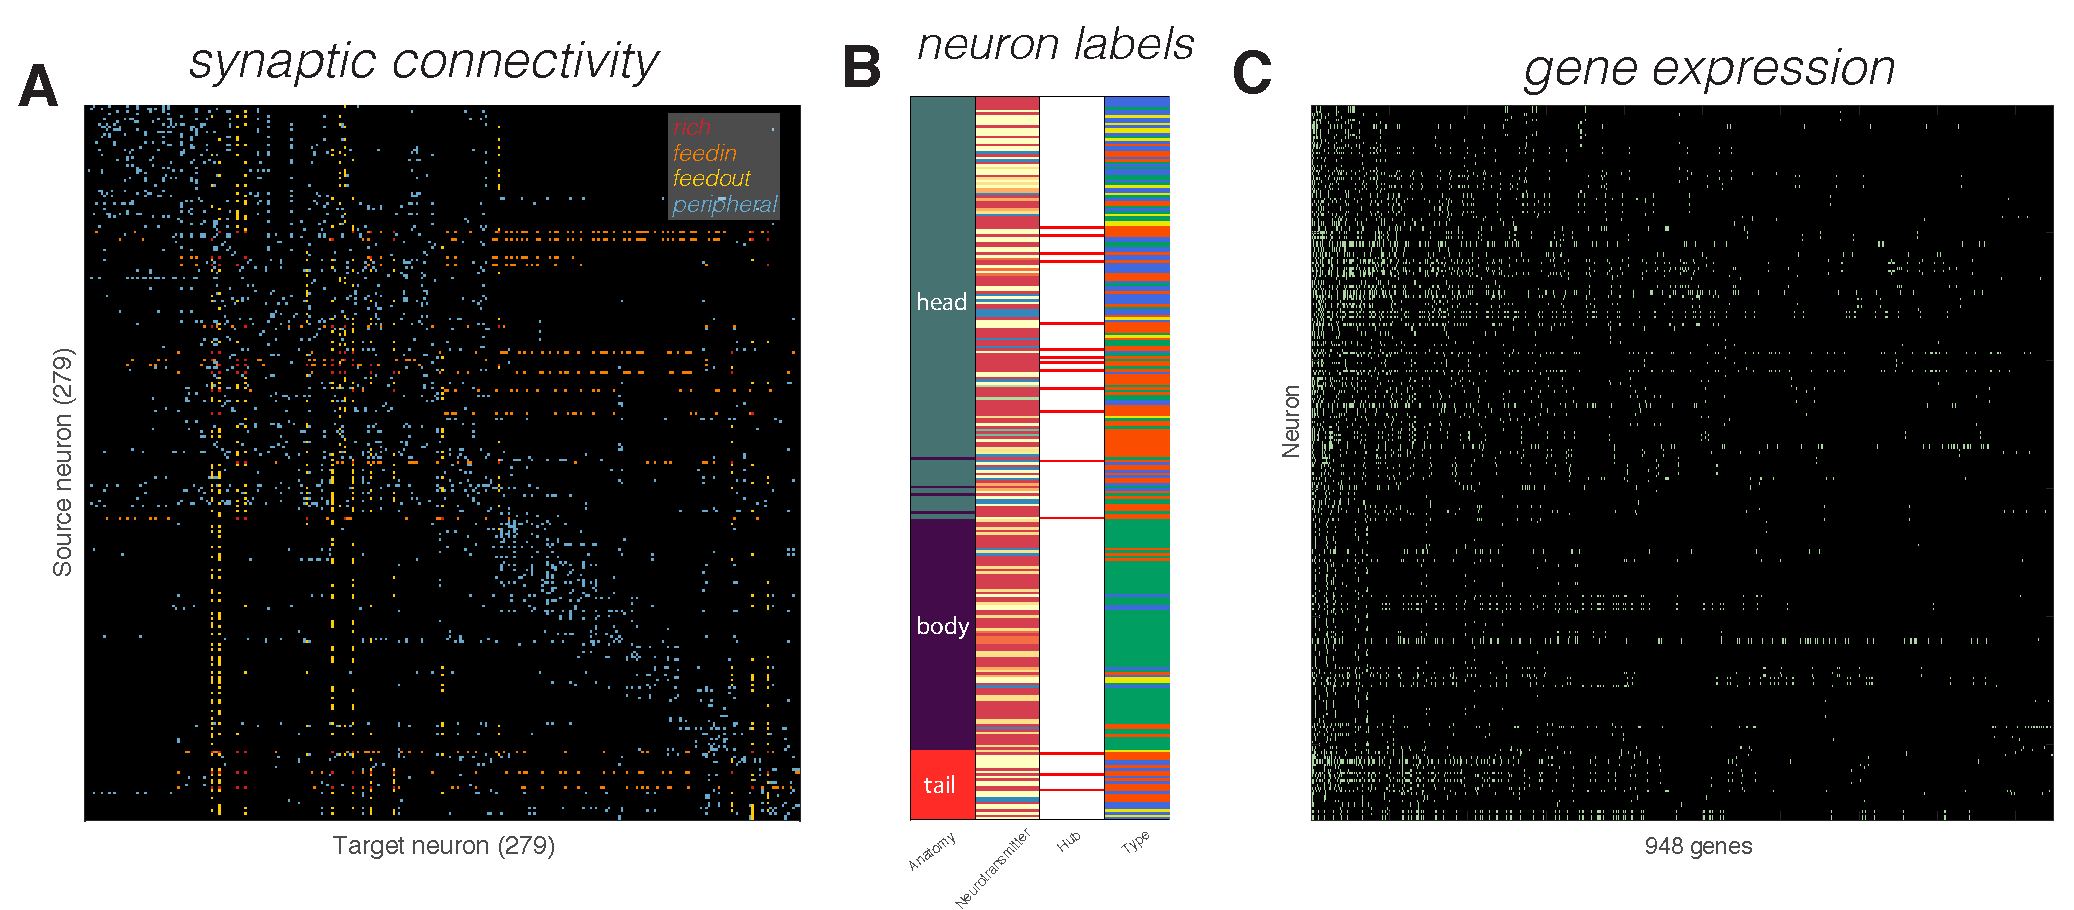
\includegraphics[width=1\textwidth]{SchematicIndicators.pdf}
 \caption{\textbf{Schematic representation of the data used in this study.}
All plots show neurons (rows) ordered by anterior-posterior along the longitudinal axis, from the top of the head (upper, left) to the bottom of the tail (lower, right).
%Schematic representation of the \textit{C. elegans} nervous system is shown on the left (scale of the animal is not preserved).
(A) Connectivity matrix summarized 2990 directed chemical and electrical connections between 279 neurons from neuron $i$ (row) to neuron $j$ (column).
Connections are colored according to how they connect hubs ($k > 44$) and nonhubs ($k \leq 44$), as `rich' (hub $\rightarrow$ hub), `feed-in' (nonhub $\rightarrow$ hub), `feed-out' (hub $\rightarrow$ nonhub), and `peripheral' (nonhub $\rightarrow$ nonhub).
(B) Neurochemistry (types as labeled), anatomical location (as labeled), birth time (from early born neurons, black, to late-born neurons, white), hub assignment (hubs labeled red), and functional type (as labeled).
% The 948 genes (columns) are expressed in each of the a neuron that are expressed in at least one neuron.
(C) Binary gene expression indicated as a green dot when a gene (column) is expressed in a neuron (row).
%[[TODO: Would be nice to put neuronal metadata on the edge (if clear enough to read) -- could perhaps remove the CGE plot?]]
%[[TODO: Add information about and permission for the head-tail diagram.]]
%[[TODO: Add labels about head/tail because the data don't actually follow the spatial scale shown on the left]]WHY SHOW the picture of the worm then?
}
\label{fig:Fig1}
\end{figure}
% ------------------------------------------------------------------------------

Our analysis is presented in five parts:
(i) given past evidence for a major effect of physical distance on connection probability and CGE \cite{Fulcher:2016ck}, we first characterize the spatial dependency of connection probability and CGE;
(ii) we confirm the rich-club organization of the \emph{C. elegans} connectome;
(iii) we show that CGE is increased in connected pairs of neurons relative to unconnected pairs, in electrical synapses relative to chemical synapses, and in connected hub neurons relative to other types of connected neuron pairs (mirroring previous results in the mesoscale mouse connectome \cite{Fulcher:2016ck});
(iv) we demonstrate that high CGE between connected hub neurons is not driven by factors like stereotypical interneuron expression, birth time, lineage similarity, neuromodulator types or expression similarity within modules, but may be driven by the high CGE of command interneurons;
(v) we characterize the contribution of specific genes, and broader gene ontology categories, to the observed patterns.
% we show that these transcriptional signatures may be driven by glutamate receptor signaling, and that
% Consistent with previous results in the mouse \cite{Fulcher:2016ck}, we show that synaptically connected neurons display more similar gene expression than those that are unconnected, and that, amongst connected regions, those involving hub neurons show more similar gene expression.


\subsection*{Spatial dependency}
Previous work has demonstrated the importance of spatial effects in driving patterns of gene expression, with more proximal brain areas exhibiting more similar gene expression patterns than more distant brain areas \cite{Krienen:2016eq, Fulcher:2016ck, Pantazatos:2016ir, Richiardi:2017hb}.
Connection probability also decreases with spatial separation between:
brain areas \cite{Horvat:2016ia, Wang:2016gg, Markov:2013jo, Henderson:2014fg, Fulcher:2016ck, Noori:2017ce},
individual neurons in mouse primary auditory cortex \cite{Levy:2012dy},
and neurons of the \emph{C. elegans} nervous system (cf. Fig.~S1 of \cite{Azulay:2016cg}).
Unlike network analyses of mammalian brains, where all neurons are confined to a spatially contiguous organ, neurons of the \emph{C. elegans} nervous system are distributed throughout the entire organism, forming a dense cluster of 147 neurons in the head (all within 130\,$\mu$m), 105 sparser neurons in the body (spanning 1.02\,mm), which are predominantly motor neurons (75\%), and another dense cluster of 27 neurons in the tail (all within 90\,$\mu$m of each other), as plotted in Fig.~\ref{fig:Fig2}.
In order to examine the relationship between connectivity and CGE, we first need to understand the spatial dependence of both connectivity and CGE to characterize the extent to which previously reported spatial dependencies of these measurements apply to the microscale nervous system of \emph{C. elegans}.
% To ensure that relationships between connectivity and gene expression are not driven by their mutual spatial dependency,

% The connection probability for pairs of neurons decays sharply as a function of the physical distance between them, excluding connections between the body and head, and between the body and tail, cf. Figs.~\ref{fig:Fig3}A,B), mirroring recent results of mesoscale mammalian brains, in mouse \cite{Goulas:2016hr, Fulcher:2016ck}, and rodents and primates \cite{Horvat:2016ia}.

% ------------------------------------------------------------------------------
% <<VisRichConns>>
\begin{figure}[h]
\centering
    %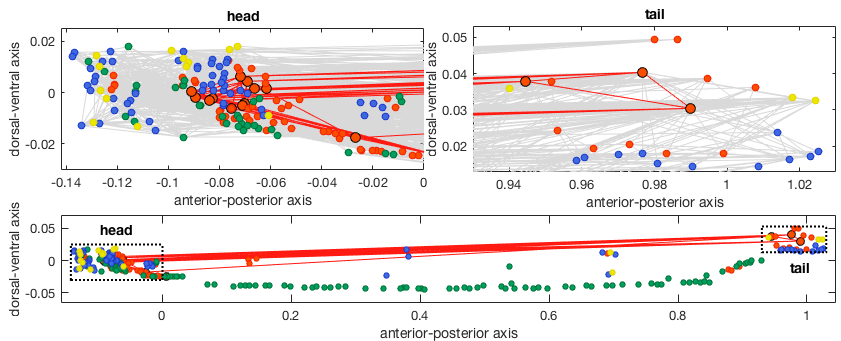
\includegraphics[width=1\textwidth]{SpatialPlotAnnotated.png}
\caption{
\textbf{Hub neurons are contained within the head and tail of \emph{C. elegans}}.
Neurons are positioned along the anterior--posterior (horizontal), and dorsal--ventral (vertical) axes, and are colored by type:
(i) interneuron (85 neurons, orange),
(ii) sensory (68 neurons, blue),
(iii) motor (108 neurons, green), or
(iv) multiple assignments (18 neurons, yellow).
Hub neurons (i.e., neurons with $k > 44$, see Fig.~\ref{fig:Fig5}) are shown as larger circles and outlined in black.
`Rich-club' connections between hub neurons are shown (red), and all other connections are also shown in the upper plots (gray).
Axes of each subplot are to scale with each other, and the upper zoomed-in plots of the head and tail are shown as dotted rectangles in the lower plot.
\label{fig:Fig2}
}
\end{figure}
% ------------------------------------------------------------------------------

We first characterize the probability that two neurons will be connected given their source and target types, labeling each neuron as being in either the `head', `body', or `tail' of \emph{C. elegans}.
% (cf. Fig.~\ref{fig:Fig2}).
Connection probability is plotted as a function of Euclidean separation distance in Fig.~\ref{fig:Fig3} for each combination of source and target neuron labels, across 10 equiprobable distance bins (with exponential fits added for visualization).
Distinguishing connections by source and target neuron types uncovers clear spatial relationships (that are obscured when all connections are grouped, as in \cite{Azulay:2016cg}), that differ across connection classes.
From the very short distance scale of $\lessapprox 100\,\mu$m of head$\rightarrow$head and tail$\rightarrow$tail connections to the very longest-range head$\rightarrow$tail and tail$\rightarrow$head connections ($\gtrapprox 1\,$mm), connection probability decreases with separation distance (Fig.~\ref{fig:Fig3}A).
For connections between pairs of neurons located in the body, ranging up to $\approx 1$\,mm, a near-exponential trend is exhibited, mirroring results in other species and across longer length scales \cite{Wang:2016gg}, including mouse \cite{Goulas:2016hr, Fulcher:2016ck}, and in rodents and primates \cite{Horvat:2016ia}.
Other connections do not exhibit strong spatial connectivity relationships, i.e., connections between the body and head or between the body and tail, shown in Fig.~\ref{fig:Fig3}B.
% [[Is this expected? Are head and tail, and neurons within the body somehow functionally distinct units that you would expect to exhibit different connectivity relationships compared to connections between the body and head or tail?? Would be nice to add some speculative sentence here around this.]]

% ------------------------------------------------------------------------------
% <<plotSpatialEffectsMain.m>>
% ------------------------------------------------------------------------------
\begin{figure}[h]
  \centering
    %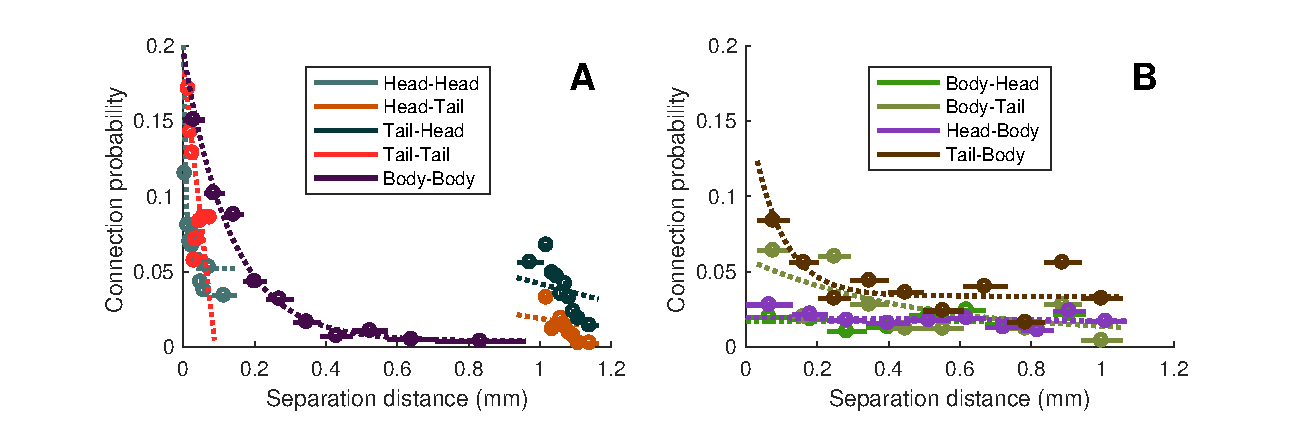
\includegraphics[width=\textwidth]{connectionProbability.eps}
  \caption{
\textbf{Connection probability decreases with separation distance within and between the head and tail, and within the body.}
The connection probability for a pair of neurons as a function of their Euclidean distance is estimated in 10 equiprobable distance bins, shown as a circle (bin centers) and a horizontal line (bin extent).
There is a decreasing relationship for connections: within the head (aqua), from head$\rightarrow$tail (brown) and from tail$\rightarrow$head (stone blue), within the tail (red), and within the body (dark purple).
Exponential fits of the form $f(x) = A\exp(-\lambda x) + B$, some of which appear approximately linear across the range of the data, are shown as dotted lines.
(B)
Plots as in (A), but for connection classes between the body and head/tail: from body$\rightarrow$head (forest green), from body$\rightarrow$tail (dirt green), connections from head $\rightarrow$ body (purple), and from tail$\rightarrow$body (dark brown).
Apart from a small effect at short range for tail$\rightarrow$body connections, these connection classes show minimal distance dependence.
% A decreasing relationship is evident up to a separation distance of approximately 0.2\,mm (driven by tail-tail and head-head connections), with a longer-range decrease up to $\approx$0.5\,mm due to body-body connections.
% The increase at large distances ($\approx 1$\,mm) is due to head-tail connections, which also show a decay with distance, from $\approx 1$\,mm through to $\approx$1.2\,mm.
% connections between body and head and body and tail showed no clear distance dependence.}
  }
  \label{fig:Fig3}
\end{figure}

% The probability of a pair of neurons being connected decreases as a function of their separation distance for connections within the head, connections within the tail, connections within the body, and connections between the head and tail

We next investigate the dependence of CGE, $r_\phi$, on the separation distance between neuron pairs, shown in Fig.~\ref{fig:Fig4}.
% (excluding bilateral pairs of neurons)
CGE decreases slightly with separation distance for the spatially close neurons within the head (Fig.~\ref{fig:Fig4}A) and within the tail (Fig.~\ref{fig:Fig4}B), but not for pairs of neurons involving the body (Fig.~\ref{fig:Fig4}C).
% Stronger spatial relationships were seen within the head for specific subtypes of neurons, including pairs of interneurons, pairs of sensory neurons, pairs of motor neurons, and motor-interneuron pairs (Figs~\ref{fig:S_distCoexp}D--H).
% Within the head, a decreasing (approximately exponential) underlying trend could be seen for pairs of interneurons, pairs of sensory neurons, pairs of motor neurons, and motor-interneuron pairs (Figs~\ref{fig:S_distCoexp}D--H).
% [[Add some interpretation in terms of the function of body neurons as potentially distinct from those in the head and tail??]].
% Furthermore, $r_\phi$ is not symmetric about a trend line; rather the trends that exist for head neurons and tail neurons are driven by pairs of close neurons with high CGE.
The decreasing trend in CGE with distance within the head and tail is primarily driven by a subset of nearby neurons with high $r_\phi$.
It may therefore represent a relationship specific to particular functionally related neurons, rather than a general, bulk spatial relationship seen in macroscopic mammalian brains \cite{Fulcher:2016ck}.
% Given the weak spatial relationships of $r_\phi$ in \emph{C. elegans} that are only seen within the head and tail and are driven mostly by pairs of close neurons with similar gene expression profiles, there is no clear bulk spatial trend that can be corrected for (as done previously for mouse brain expression data \cite{Fulcher:2016ck}).
% Residuals after subtracting an exponential form (following Fulcher and Fornito using mouse brain expression data \cite{Fulcher:2016ck}), are not symmetric, since the trend is often driven by pairs of close neurons with high CGE.
Accordingly, attempting to correct for a bulk, non-specific trend by taking residuals from an exponential fitted to the relationship produced artifactual reductions in the CGE of many neuron pairs (shown in \nameref{S3_Fig}).
% NOTE AA: I think we should include the plot (probably in supp) where exp for head-head is fitted (A) and a plot for residuals (B).
% Given that the effect was relatively small, and no standard correction could be applied, we use original uncorrected CGE data for all the further analyses.
% Due to the large artifacts introduced, we chose not to correct for the small spatial dependence of CGE in head-head and tail-tail connections for the main analyses presented here,
Thus, we found no evidence for bulk spatial relationships of $r_\phi$ in the neuronal connectome of \emph{C. elegans}.
% and accordingly analyze $r_\phi$ without any bulk spatial correction throughout this work.
% , but note that applying such a correction yields similar results to those presented.
% [[TODO: INCORPORATE RESULTS/VERIFICATION, cf. \emph{CoExpressionDistanceCorrect}]].
% Future data that allow more accurate and continuous measurement of CGE, may allow spatial correction to be applied more accurately.
% However, because we found no correlation between Euclidean distance between a pair of neurons (based on their two-dimensional coordinates) and their CGE in the C. elegans nervous system (Fig.~\ref{fig:S_distDep}), no correction was necessary here.
% In \textit{C. elegans}, we found a semi-exponential relationship between connection probability and Euclidean separation distance (based on their two dimensional coordinates) between a pair of neurons, but no correlation between the Euclidean separation distance between a pair of neurons and their CGE, $r_\phi$.

% ------------------------------------------------------------------------------
% <<coexpressionDistance(C,G)>>
% ------------------------------------------------------------------------------
\begin{figure}[h]
  \centering
%    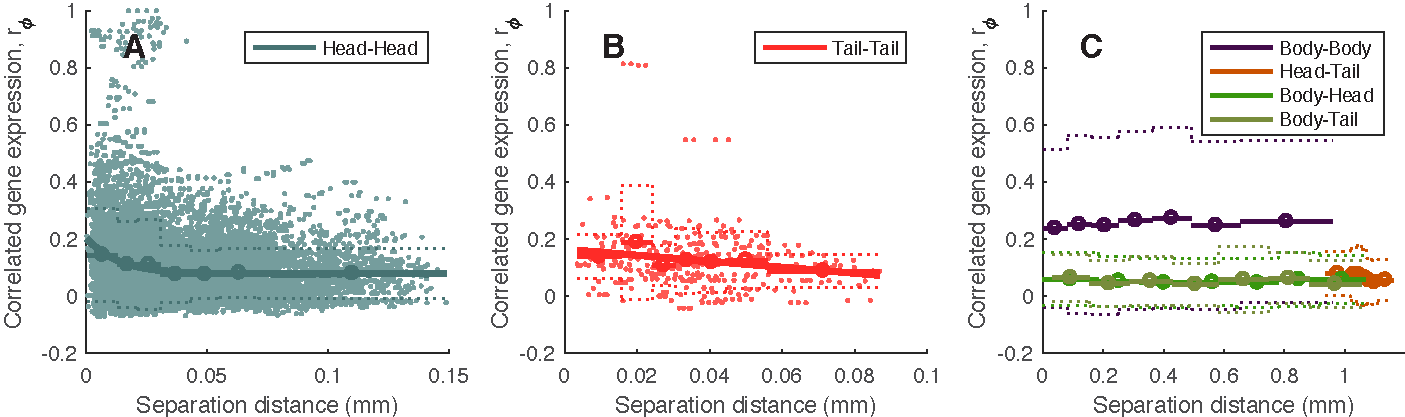
\includegraphics[width=\textwidth]{spatialCoexpressionMain.pdf}
  \caption{
  \textbf{Dependence of correlated gene expression, $r_\phi$, on spatial separation between pairs of neurons.}
  Correlated gene expression, $r_\phi$ (excluding bilateral homologous pairs of neurons), is shown as a function of the pairwise separation distance between pairs of neurons (shown as the mean (solid) $\pm$ standard deviation (dotted) in seven equiprobable distance bins, with extent shown as horizontal bars), for (A) all pairs of neurons in the head, (B) all pairs of neurons in the tail, and (C) all other pairs (labeled).
  Scatters for all neuron pairs are added in (A) and (B).
  An exponential relationship, $f(x) = A\exp(-\lambda x) + B$, is fitted in (A) and (B).
  The weak decreasing trend in $r_\phi$ with distance, is primarily driven by a small subset of nearby neurons with high $r_\phi$, and may therefore represent a more specific relationship between particular neurons, rather than a general, bulk spatial relationship observed in macroscopic mammalian brains \cite{Fulcher:2016ck, Krienen:2016eq}.
\label{fig:Fig4}
  }
\end{figure}


% Although distance slightly influenced CGE, especially for very closely positioned neurons within the head, exponential form could not explain the relationship.
% However, the spatial effect in this neuronal nervous system is much smaller here than in the mouse brain \cite{Fulcher:2016ck}, and concentrated on restricted spatial scales of the head (and tail).


\subsection*{Hub connectivity}

%% INTRODUCE RICH CLUB  hene and focus on the difference between rich/feeder/peripheral links below
% [[TODO: Shorten section, focusing on reproducing Towlson]]
% \paragraph{Rich club organization of the connectome}

% <<hubs>>
Next we analyze the topological properties of the \emph{C. elegans} connectome, represented as a directed, binary connectivity matrix between 279 neurons, combining directed chemical synapses and undirected electrical gap junctions (Fig.~\ref{fig:Fig1}).
% between 279 neurons.
 % of 2194 chemical connections between 279 non-pharingeal neurons (1961 pairs of connected neurons) \cite{Varshney2011}, focusing particularly on hub connectivity.
The degree distribution is shown in Fig.~\ref{fig:Fig5}A, where neurons are distinguished by type: 68 sensory neurons, 85 interneurons, 108 motor neurons, and 18 neurons with multiple assignments.
Consistent with the results of Towlson et al., who used an undirected version of the connectome (by ignoring the directionality of chemical synapses), we found a positively-skewed degree distribution containing an extended tail of high-degree hub interneurons.
% Note that we define degree as the sum of incoming and outgoing projections to a given neuron (total degree, $k$).
% who included both synaptic connections as well as gap junctions and symmetrized the directed synaptic connectivity (despite only 233 out of 1\,961 pairs of connected neurons being reciprocally connected), whereas here we retain the directed architecture of the connectome
Hub interneurons of \emph{C. elegans} are mostly command interneurons and mediate behaviors like coordinated locomotion and foraging \cite{tsalik2003}.
% connectivity between interneurons in the rich club provides the anatomical basis for vital neuronal computation of behaviours, such as coordinated locomotion and foraging36,37. Forward and backward movements, for example, are generated in two functionally separate subsets of neurons in this core, potentially coordinated through reciprocal inhibi- tion37,44. Moreover, a study recently demonstrated that random search behaviour in the worm can be approx- imated by a connectome-based stochastic model of this circuit4

% Here we confirm the high connectivity, centrality and wiring cost of hub connections in the C elegans connectome, as previoulsy shown by Towlson et al () and as also found in the macaue (Harriger) and human (van den Huevel-PNAS) brains.
% We show RC organization... and show hubs are interneurions...
% We show cost and centrality (may be worth including a curve for betweenness)


% ------------------------------------------------------------------------------
% <<TopologyFigures.m>>
% ------------------------------------------------------------------------------
\begin{figure}[h]
   \centering
%    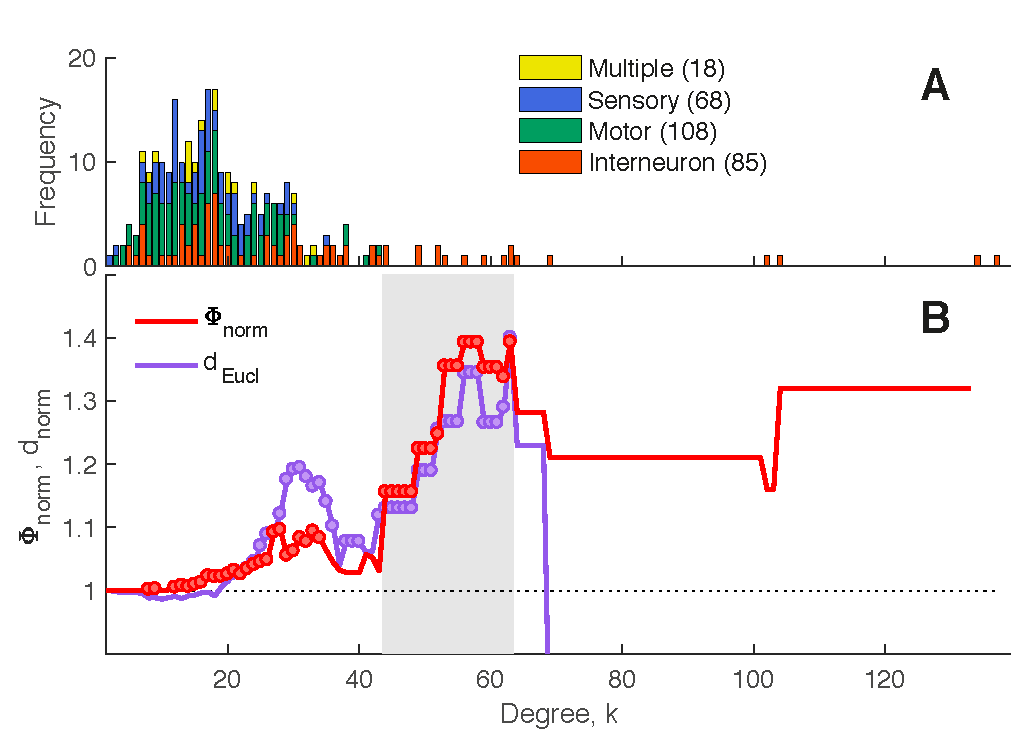
\includegraphics[width=0.9\textwidth]{topologicalRCall2.pdf}
    % 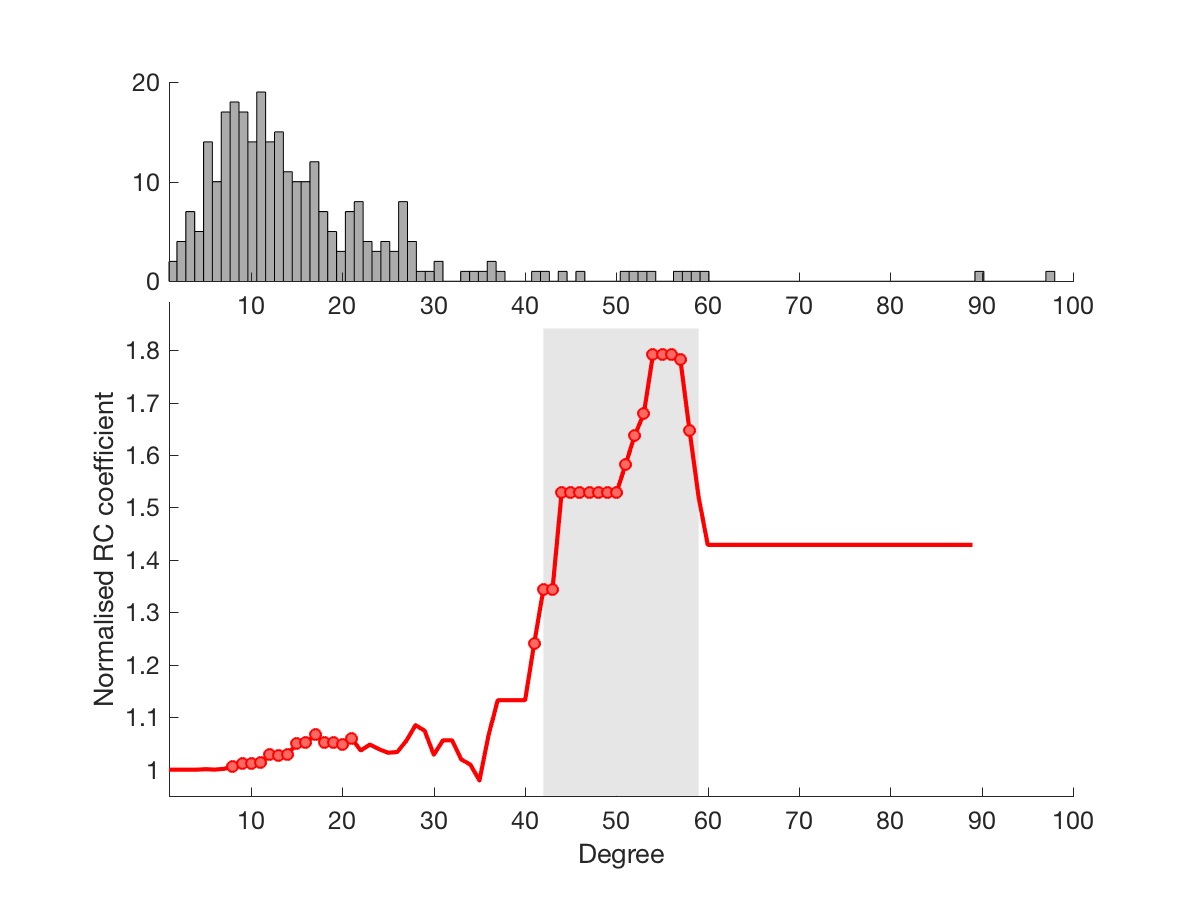
\includegraphics[width=0.7\textwidth]{RCcurve.eps}
 \caption{\textbf{Rich-club organization of the \emph{C. elegans} connectome}.
% A: Topological rich-club. B: Mixed rich-club. C: Weighted rich-club.
(A) Degree distribution of neurons, labeled to four categories:
(i) interneuron (85 neurons, orange),
(ii) motor (108 neurons, green),
(iii) sensory (68 neurons, blue), or
(iv) multiple assignments (18 neurons, yellow).
The distribution features an extended tail of high-degree interneurons.
(B)
Normalized rich club coefficient, $\Phi_\mathrm{norm}$ (red), as a function of the degree, $k$, at which hubs are defined (as neurons with degree $>k$).
Also shown is the mean Euclidean separation distance, $d$ (purple) between connected hub regions (across degree thresholds, $k$).
$\Phi_\mathrm{norm} > 1$ indicates that hubs are more densely interconnected among each other than expected by chance, with red circles indicate values of $\Phi_\mathrm{norm}$ that are significantly higher than an ensemble of 1\,000 degree-matched null networks ($p < 0.05$).
Purple circles indicate where the Euclidean distance between connected pairs of hubs is significantly greater than the Euclidean distance for all other pairs of connected regions (right-tailed Welch's $t$-test, $p < 0.05$).
%[[TODO: Also suggest replacing red with one of these, since red is used in CGE plot to represent something different]]
%[[TODO: Add right-side vertical-axis to give units for distance]]
}
 \label{fig:Fig5}
 \end{figure}
% ------------------------------------------------------------------------------


% ------------------------------------------------------------------------------
% <<rich-club organization>>
% ------------------------------------------------------------------------------
Using the normalized rich-club coefficient, $\Phi_\mathrm{norm}$, to quantify the extent to which hubs are densely interconnected, we confirmed the results of Towlson et al. \cite{Towlson2013}, finding rich-club organization in the connectome, as shown in Fig.~\ref{fig:Fig5}B.
% , with $\Phi_\mathrm{norm} > 1$ indicating rich-club organization of the network.
% Rich-club organization of the \emph{C. elegans} connectome was first demonstrated by Towlson et al. \cite{Towlson:2013gf}.
%and exclude gap junctions (to prevent them contributing to a different gene expression signature).
% Specifically, we find that
% Adj = GiveMeAdj(C,'zeroBinary','ch');
% reciprocal: sum(sum(Adj & Adj'))/2 = 233
% unidirectional: sum(sum(Adj & ~Adj')) = 1728
% either: sum(sum(Adj | Adj'))/2 = 1961
The figure plots the variation of $\Phi_\mathrm{norm}$ across degree thresholds, $k$, at which hubs are defined (as neurons with degree $>k$), with red circles indicating a significant increase in link density among hubs relative to 1000 degree-preserving nulls (permutation test, $p < 0.05$).
% [[check whether randmio\_dir only preserves degree: AA - degree distributions in binary, out-strength (but not in-strength) in weighted]].
The plot reveals rich-club organization ($\Phi_\mathrm{norm} > 1$) at the upper tail of the degree distribution, particularly across the range $44 < k < 63$, shaded gray in Fig.~\ref{fig:Fig5}B.
% ), referred to here as the `topological rich-club regime'.
Similar results were obtained using weighted representations of the connectome (i.e., using information about the number of synapses in the connectivity network) for two different definitions of the weighted rich-club coefficient \cite{Opsahl2008}, shown in \nameref{S4_Fig}.
Throughout this work, we define a set of hubs as the sixteen neurons with $k > 44$, which corresponds to the lowest degree threshold at which the network displays a contiguous region of significant rich-club organization at high $k$.
Our list of hubs includes all of the 11 hub neurons of Towlson et al.~\cite{Towlson2013} at $3 \sigma$ (see \nameref{tab:HubList}) with five additional hubs identified in our analysis of the directed connectome.
% This indicates that when nodes are defined as hubs (degree $>\textit{k}$) in this range, they are more densely interconnected than expected by chance.
 % of the analyses presented below examine how different topological and genomic properties vary as a function of the hub threshold, $k$, but for analyses requiring a fixed hub definition, we define hubs as the 13 neurons with

% ------------------------------------------------------------------------------
% <<distance, geometric effects>>
% ------------------------------------------------------------------------------
% <<cf. NeuronTypeStats.m to run these numbers>>
The rich-club connectivity of the \emph{C. elegans} connectome is accompanied by an increase in mean hub-hub connection distance \cite{Towlson2013}, with a significant increase through the topological rich-club regime (right-tailed Welch's $t$-test, $p < 0.05$), shown in Fig.~\ref{fig:Fig5}B.
% and consistent with prior analysis by Towlson et al. \cite{Towlson:2013gf}.
 % we plot the mean distance between all pairs of connected hubs at each degree threshold, $k$.
This can be attributed to a relative increase in long-distance hub-hub connections between the head and tail, shown in Fig.~\ref{fig:Fig2} (cf. \nameref{S5_Fig}).
% , we find an increase in mean hub-hub connection distance with $k$, through to the extent of the topological rich-club regime.
The high connection density and long mean anatomical distance between pairs of hub neurons counters the general trend in the \emph{C. elegans} connectome, where the probability of connectivity between two neurons decays with their separation distance (Fig.~\ref{fig:Fig3}).
These results are consistent with previous findings across diverse neural systems and suggest that the rich club may provide a central yet costly backbone for neuronal communication in \emph{C. elegans} \cite{vandenHeuvel:2012kh, Towlson2013}.
% Towlson2013
% replicate the findings by Towlson et al. \cite{Towlson2013}, demonstrating that hub-hub connections in \emph{C. elegans} are dense and extend over significantly longer distances than other types of connections in the synaptic network of the nematode nervous system, consistent with the rich club forming a central yet costly backbone for neuronal communication \cite{vandenHeuvel:2012kh}.
% The distribution of hubs and hub-hub connections in two-dimensional space is depicted in Fig.~\ref{fig:Fig2}.

% Rich club in the chemical synapse network consists of 13 high degree neurons with degree $42 \leq k \leq 98$.
% When comparing the normalized rich club coefficient $\Phi_\mathrm{norm}$ as a function of degree in both cases we notice that $\Phi_\mathrm{norm}$ reaches slightly higher values for a directed chemical synapse connectome in the topological rich-club regime ($\Phi_\mathrm{normMAX} = 1.8$), while an increase in the symmetrized connectome is not so sharp ($\Phi_\mathrm{normMAX} = 1.4$) meaning that the  rich club effect might me slightly more pronounced in a directed version of a synaptic connectome.

% In connectomes across species and scales, degree is distributed unequally, with a small number of highly connected brain regions, known as hubs \cite{Sporns:2007ea}, that are themselves more densely connected between themselves, forming a so-called `rich club' \cite{deReus:2013cy, ZamoraLopez:2010hy, Shih:2015cu, vandenHeuvel:2012kh, vandenHeuvel:2011he}.
% The same is true in the C. elegans neuronal nervous system, analyzed in the past as an undirected binary connectome including both chemical and electrical synapses \cite{Towlson:2013gf}, which exhibits highly connected, and densely interconnected hub neurons.

%%
\subsection*{Correlated gene expression and connectivity}

% ---connectivity/CGE---
% Having characterized the topological and geometric properties of rich-club connectivity in \emph{C. elegans},
We next investigate how the network connectivity properties of \emph{C. elegans} relate to patterns of CGE, using the mean square contingency coefficient, $r_\phi$.
% (excluding bilateral pairs of neurons to ensure their high transcriptional similarity does not drive results, see \emph{Methods}).
% Note that connections between bilateral pairs of neurons display high transcriptional similarity and are excluded from this analysis, leaving 474 electrically (514-40), 1\,940 connected pairs (1\,961 - 21) and 36\,450 unconnected pairs (36\,494 - 44).
% , to define gene CGE, and excluding CGE values between homologous left/right neuron pairs, see Methods).
% , to define CGE, and excluding CGE values between homologous left/right neuron pairs, see Methods).
To test whether CGE varies as a function of connectivity, we compared the distribution of $r_\phi$ between
(i) all connected pairs of neurons, and
(ii) all unconnected pairs of neurons.
Connected pairs of neurons have more similar expression profiles than unconnected pairs (Wilcoxon rank-sum test, $p = 1.8 \times 10^{-78}$), mirroring previous results in the mesoscale mouse connectome \cite{Fulcher:2016ck}.
% (Fig.~\ref{fig:S_RFPdistributions}).
Figure~\ref{fig:Fig6}A (left) shows distributions of $r_\phi$ for:
(i) all pairs of neurons that are connected via an electrical gap junctions (474 pairs, after excluding bilateral pairs),
(ii) all pairs of neurons that are connected via reciprocal (291 pairs) and,
(iii) unidirectional chemical synapses (1721 pairs) as well as
(iv) all pairs of neurons that have neither connection (36\,450 pairs).
% This analysis involves 474 pairs of neurons connected by a gap junctions, 1\,940 pairs connected by a synapses, and 36\,450 pairs with no connection (after excluding bilateral pairs of neurons).
Note that 175 pairs of neurons are connected both by a chemical synapse and by a gap junction, and are thus included in both chemical and electrical categories.
Amongst connected pairs of neurons, those connected via gap junctions exhibit more similar gene expression profiles than those connected via chemical synapses (Wilcoxon rank-sum test, $p = 5.4 \times 10^{-22}$).
% At the same time there is no significant difference in pairwise distances between them (Wilcoxon rank-sum test, $p = 0.63$), therefore, the increase in CGE for neurons connected via gap junctions could not be attributed to their spatial position.
% and  and chemically connected neuron pairs are not mutually exclusive with 175 pairs of neurons connected via both types of connections.
% Note that because connections between bilateral pairs of neurons display high transcriptional similarity and are excluded from this analysis, leaving 474 electrically (514-40), 1\,940 connected pairs (1\,961 - 21) and 36\,450 unconnected pairs (36\,494 - 44).
We found no difference in CGE between pairs of neurons connected reciprocally by chemical synapses ($N_1 \leftrightarrow N_2$ for two neurons $N_1$ and $N_2$) versus those connected unidirectionally ($N_1 \rightarrow N_2$) (Wilcoxon rank-sum test, $p = 0.99$), in contrast to significant differences found in the mesoscale mouse connectome \cite{Fulcher:2016ck}.
% into three distinct categories: electrical, chemical reciprocal ($X \leftrightarrow Y$) and chemical unidirectional ($X \rightarrow Y$), however, unlike in the mouse brain, we found no differences in CGE, $r_\phi$, between chemical unidirectional and reciprocal connections (see Fig.~\ref{fig:S_RFPdistributions}).


% ------------------------------------------------------------------------------
% <<coexpConnUncon.m>>
% <<RichClub.m>>
% ------------------------------------------------------------------------------
 \begin{figure}[h]
 \centering
%    \includegraphics[width=0.8\textwidth]{MeanCoexpression5.pdf}
\caption{{\bf Correlated gene expression varies as a function of connectedness and connection type.}
(A) \textit{Left}: distribution of CGE for (i) pairs of neurons connected by gap junctions, (ii) pairs of neurons connected by reciprocal chemical synapses, (iii) pairs of neurons connected by unidirectional chemical synapses, (iv) pairs of neurons that are unconnected, shown as a violin plot, with the median of each distribution represented by a horizontal line.
CGE is increased in connected (electrical or chemical; reciprocally or unidirectionally) pairs of neurons relative to unconnected pairs ($p = 1.8 \times 10^{-78}$, Wilcoxon rank sum test).
Among connected pairs of neurons neurons connected via gap junctions have more similar CGE than connected via chemical synapses (Wilcoxon rank-sum test, $p = 5.4 \times 10^{-22}$).
\textit{Right}: GCE for pairs of neurons labeled as peripheral, feed-in, feed-out, and rich, where hubs are neurons with degree $k>44$. The median of each distribution shown as a horizontal line.
% Connections between symmetrical (left/right) pairs of neurons are excluded from the analysis.
CGE is significantly higher between hubs (rich links) compared to feeder ($p = 5 \times 10^{-22}$, Wilcoxon rank sum test) and peripheral ($p = 3.9 \times 10^{-19}$, Wilcoxon rank sum test) links.
Feed-out links show significantly higher CGE than both feed-in ($p = 1.9 \times 10^{-6}$, Wilcoxon rank sum test) and peripheral links ($p = 4.5 \times 10^{-12}$, Wilcoxon rank sum test).
% Coexpression, $r_\phi$, is increased in connected compared to unconnected pairs of neurons ($P < 10^{-78}$, Wilcoxon rank sum test).
% Coexpression, $r_\phi$, is increased in neuron pairs connected via electrical synapses compared to pairs connected via chemical synapses ($P < 10^{-22}$, Wilcoxon rank sum test).
(B)
\emph{Top}: Degree distribution, $k$, of the \emph{C. elegans} connectome.
\emph{Middle}: proportion of connections that are:
`rich' (hub$\rightarrow$hub, red),
`feed-in' (nonhub$\rightarrow$hub, yellow),
`feed-out' (hub$\rightarrow$nonhub, orange), or
`peripheral' (nonhub$\rightarrow$nonhub, blue) as a function of the degree threshold, $k$, used to define hubs.
Note that at high $k$ most neurons are labeled as nonhubs and hence the vast majority of connections are labeled `peripheral'.
 \emph{Bottom}: Median CGE, $\tilde{r}_\phi$, for each connection type as a function of $k$.
The median CGE across all network links is shown as a dotted black line; the topological rich-club regime (determined from the network topology, cf. Fig.~\ref{fig:Fig5}) is shaded gray.
Circles indicate a statistically significant increase in CGE in a given link type relative to the rest of the network (one-sided Wilcoxon rank-sum test, $p < 0.05$).
%[[TODO: add labels A, B; label connection types rich, feed-in, etc.]]
}
 \label{fig:Fig6}
\end{figure}
% ------------------------------------------------------------------------------

% ---HUB CGE---
We next investigated whether CGE varies across different types of connections defined in terms of their hub connectivity.
% , focusing particularly on the role of densely interconnected hub neurons.
% characterized above, hypothesizing an increase in connections involving hubs, with hub-hub connections displaying the most similar gene expression patterns \cite{Fulcher:2016ck}.
% Given the importance of hub neurons across species [[Ref]], and previous results in the mesoscale mouse connectome \cite{Fulcher:2016ck},
For a given hub threshold, $k$, we first labeled each neuron as either a `hub' (nodes with degree $> k$) or a `nonhub' (degree $\leq k$), and then labeled each connection as either `rich' (hub $\rightarrow$ hub), `feed-in' (nonhub $\rightarrow$ hub), `feed-out' (hub $\rightarrow$ nonhub), or `peripheral' (nonhub $\rightarrow$ nonhub).
% [[TODO: Establish whether we're computing pairs of hubs (e.g., for `rich'), or for every connection between any pair of hubs -- i.e., do reciprocal connections contribute twice to the distribution at each $k$? AA: as in original mouse analysis -- all connections, but we take mean, so the mean doesn't change in either way]]
The median CGE, $\tilde{r}_\phi$, of each of these four connection types is plotted in Fig.~\ref{fig:Fig6}B, with circles indicating statistically significant increases of a given connection type relative to all other connections (one-sided Wilcoxon rank-sum test, $p < 0.05$).
Correlated gene expression in rich connections increases with degree, $k$, particularly in the topological rich-club regime where hubs are densely interconnected (shaded gray in Fig.~\ref{fig:Fig6}B).
In this topological rich-club regime, both feed-in and feed-out connections exhibit increased CGE relative to peripheral connections, which show the lowest levels of CGE.
%]][[TODO-AA: Seems like feed-in actually the lowest now??]].
Full distributions of $r_\phi$ for each edge type at a hub threshold of $k > 44$ are in Fig.~\ref{fig:Fig6}A (right).
This plot shows that, compared to all different types of pairs of neurons, connected pairs of hubs showed the highest CGE.

In summary, our results reveal:
(i) increased CGE in connected pairs of neurons;
(ii) the highest CGE in rich connections; and
(iii) lowest CGE in peripheral connections.
These results, obtained using incomplete binary annotations of gene expression across 948 genes in a microscale neuronal connectome, are consistent with a prior analysis of the expression of over 17\,000 genes across 213 regions of the mesoscale mouse connectome \cite{Fulcher:2016ck}.
% (iii) intermediate CGE in feeder connections; and

\subsection*{Potential drivers of elevated correlated gene expression between hubs}
The sixteen hub neurons in \emph{C. elegans} ($k > 44$)
are all interneurons;
are all located in either the head or tail;
are mostly contained within a single topological module of the network;
are mostly cholinergic (13/16);
and are all born prior to hatching.
% and concentrated in the head (10/13),
% \cite{Varier2011}, \cite{Pereira:2015er}
% Having demonstrated that CGE is elevated for connected regions, and particularly for connected pairs of hubs,
We therefore investigated whether the similarity of gene expression profiles between hubs is specific to their high levels of connectivity, or whether it could instead be driven by these other characteristics.
% We thus investigated whether any of these types of homogeneities amongst hub neurons could contribute to our finding of increased CGE, $r_\phi$.
% , namely modular organization, lineage similarity, or neurotransmitter type, could explain our results.

% \paragraph{Distance}).
% Implementing the same methods as previously used in CGE analysis at each degree threshold for each link type (rich, feeder, peripheral) we calculated the mean connection distance.
% Connection distance increased with increasing degree for both rich and feeder links while peripheral connections demonstrated no increase through the whole range of thresholds (Fig.~\ref{Distance}).
% Given this result, it is safe to say that increased CGE for hub-related links is not determined by lower connection distance between them as the contrary is shown to be true.

%\begin{figure}[!h]
%\centering
 %   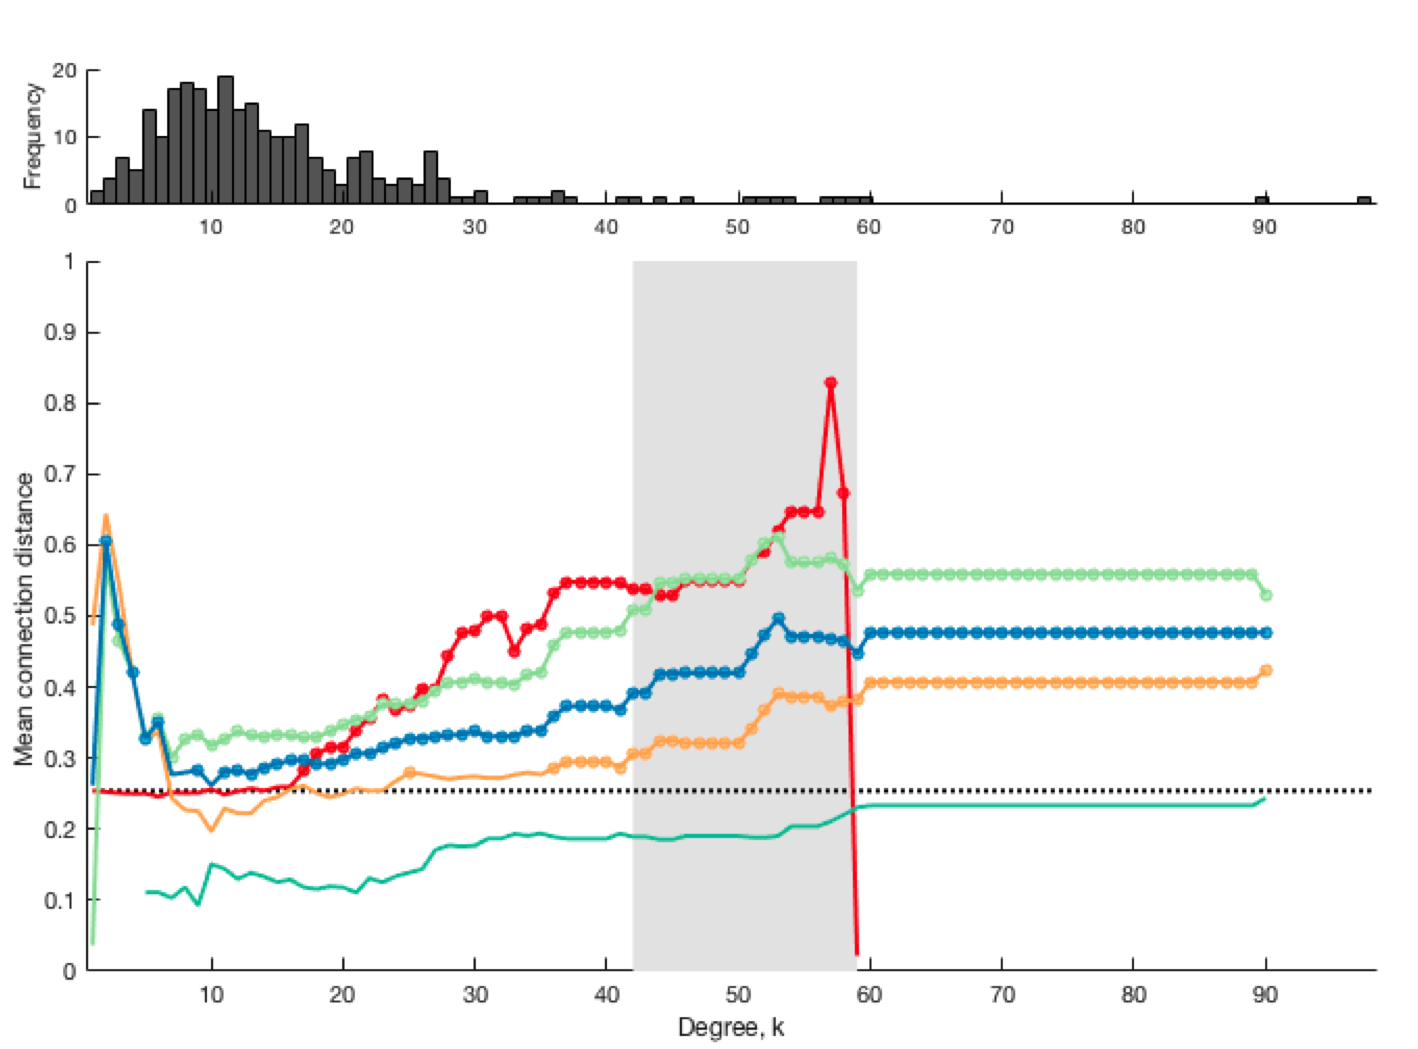
\includegraphics[width=0.7\textwidth]{distance_k}
 %\caption{{\bf Connection distance as a function of degree}}
 %\label{Distance}
 %\end{figure}

\paragraph{Interneurons.}
The sixteen hubs in \textit{C. elegans} are all interneurons.
To determine whether the increase in CGE in rich connections was specific to interneurons, we plotted the median CGE for hub-hub connections, $\tilde{r}_\phi$, as a function of the degree threshold, $k$, separately for connections involving interneurons, sensory neurons, and motor neurons, as shown in Figs.~\ref{fig:Fig7}B.
For the curve labeled `sensory', for example, each point is the median $\tilde{r}_\phi$ across connections involving sensory neurons (i.e., at least one neuron of a connected pair is a sensory neuron), for which both neurons have degree $>k$.
The increase in median hub-hub CGE is strongest for connections involving interneurons.
Motor neurons show a smaller increase with $k$, although the absence of motor and sensory neurons with high {$k$ makes it difficult to draw firm conclusions.
However, we do find that CGE is higher for hub-hub pairs of interneurons compared to connections between all pairs of nonhub interneurons (Wilcoxon rank sum test, $p = 5 \times 10^{-21}$), indicating that the high CGE of rich pairs cannot simply be explained by the fact that all hub neurons are interneurons (Fig.~\ref{fig:Fig7}C).
We next investigated whether greater CGE of hub-hub pairs of neurons could be driven by specific anatomical properties of hub interneurons.
Specifically, we selected a subset of nonhub interneurons that most closely resemble the anatomical properties of hub interneurons in terms of their position and projection pattern; that is, the cells are in similar locations in the head and their axons project to similar targets in the tail. These neurons were AVFL, AVFR, AVHL, AVHR, AVKR, AVJL, and AVJR.
Pairs of hub interneurons show higher median CGE than pairs of anatomically-matched nonhub interneurons, with the difference being at the threshold of statistical significance (Wilcoxon rank sum test, $p = 0.051$), suggesting that the increase in CGE amongst hub interneurons cannot be explained by their anatomical similarity among interneurons.

% ------------------------------------------------------------------------------
% <<plot_neuronType.m>>
% ------------------------------------------------------------------------------
\begin{figure}[h]
\centering
%   \includegraphics[width=1\textwidth]{Type_Degree5NEW.pdf}
 \caption{
\textbf{Correlated gene expression is highest for hub interneurons.}
(A) The number of connected neuron pairs involving interneurons (orange), sensory neurons (blue), and motor neurons (green) across degree threshold, $k$, represented as $\log_{10}$(number of links).
(B) Median CGE as a function of degree for connections involving different types of neurons.
Circles indicate a statistically significant increase in CGE in a given link type relative to the rest of the network (one-sided Wilcoxon rank-sum test, $p < 0.05$).
(C) CGE distributions for connected pairs of hub interneurons (red) and connected pairs of non-hub interneurons (dark yellow) (Wilcoxon rank sum test, $p = 5 \times 10^{-21}$). * represents statistically significant difference.
%[[TODO-AA: Is the top-left plot actually counting pairs?? Or is it actual connectome edges?]] - pairs (changed in caption)
%[[TODO-AA: Clarify axis tick labels in B: at the moment appears like a node-level analysis on horizontal axis but pairwise analysis on vertical]]
%[[TODO-AA: Recolor, or somehow update caption for B that reflects the new command interneuron story -- will do when plots are finalized]]
}
 \label{fig:Fig7}
\end{figure}

% Neurons in \emph{C. elegans} are annotated to the following categories: sensory neurons, motor neurons, and interneurons (eighteen multifunctional neurons are annotated to two categories).
% As in Towlson et al.~\cite{Towlson:2013gf}, we find that
%All sixteen hubs ($k > 44$) in \emph{C. elegans} are interneurons. % (cf. Fig.~\ref{fig:Fig5}A).
%To determine whether the increase in CGE in rich connections was specific to interneurons, we plotted the median CGE for hub-hub connections, $\tilde{r}_\phi$, as a function of the degree threshold, $k$, separately for:
%(i) connections involving interneurons,
%(ii) connections involving sensory neurons, and
%(iii) connections involving motor neurons, as shown in Fig.~\ref{fig:Fig7}A.
% separated our CGE analysis into connections involving: (i) interneurons, (ii) sensory neurons, and (iii) motor neurons.

% Thus, the three categories are not mutually exclusive; for example, the `interneuron' class includes connections between an interneuron and any other neuron.
%We find that the increase in median hub-hub CGE, $\tilde{r}_\phi$, with $k$ is strongest for connections involving interneurons, while connections involving motor neurons show a smaller increase with $k$, and connections involving sensory neurons show no relationship.
% , which are unique in their increasing average CGE with increasing degree
% Thus, interneurons drive the CGE relationship with degree, $k$,

% Having found that interneurons drive the CGE relationship with degree, $k$,
%We next investigated whether hub neurons show a unique transcriptional signature amongst interneurons.
% compareInterneurons.m
%Pairs of hub interneurons indeed exhibit significantly higher CGE compared to pairs of all other interneurons (Wilcoxon rank sum test, $p = 5 \times 10^{-31}$).
%However, we tested whether this observed increase could be driven by the anatomical properties of hub interneurons [[TODO-AA: this still needs some unpacking to distinguish from the rank sum test just performed]].
%We selected a subset of interneurons that most closely resemble the anatomical properties of hub interneurons, in terms of their origination and termination locations, arriving at the following set of eight nonhub head interneurons: AVFL, AVFR, AVHL, AVHR, AVKL, AVKR, AVJL, and AVJR [[any reproducible criteria through which these were selected??]].
% to determine whether interneurons that are anatomically similar to hubs show a specific gene expression pattern:
% however are not required to have similar connectivity pattern.
% The distribution of CGE, $r_\phi$, between all pairs of 16 hub interneurons, and all pairs of anatomically-matched nonhub interneurons.
%To determine whether hub neurons of this anatomical type showed more similar expression patterns than nonhubs of the same type, we computed the CGE, $r_\phi$, between all pairs of hub neurons and all pairs of nonhub neurons (ignoring their connectivity for this analysis).
%As shown in Fig.~\ref{fig:Fig7}B, pairs of hub interneurons exhibit significantly higher CGE than pairs of anatomically-matched nonhub interneurons (Wilcoxon rank sum test, $p = 0.047$).
%Thus, the increase in CGE amongst hub interneurons cannot be explained simply by the fact that hubs are interneurons.
% ---even amongst interneurons with the same anatomical properties, hubs exhibit significantly increased CGE.

\paragraph{Modular organization.}
%The \emph{C. elegans} connectome has a modular organization, and can be decomposed into groups of neurons or modules with dense inter-module connectivity (with relatively sparse connectivity between modules) \cite{Kim:2014bu, Pan:2010jt, Bassett2010}, or into groups of neurons with more similar patterns of connectivity within groups than between groups \cite{Achacoso:1992ay, Pavlovic:2014gx}.
% , which can correspond to specific functional circuits
%Given that connectome modules may correspond to functionally specialized systems, it is therefore plausible that neurons belonging to the same module might exhibit similar gene expression patterns, as has been shown for macroscopic functional networks in the human brain \cite{Richiardi2015}.
%Brain network hubs generally participate in multiple modules \cite{vandenHeuvel:2013ij, deReus:2014cz}, and their dense rich-club connectivity implies that they may form their own module that overlaps with other, more specialized systems \cite{Fornito:2015dq, deReus:2013cy, ZamoraLopez:2010hy}.
%We therefore investigated whether therefore increased CGE between pairs of hub neurons in the \emph{C. elegans} connectome can be explained by their distribution across connectome modules.
Another important topological property of neural systems is modularity, whereby network nodes coalesce into tightly connected subsystems that are thought to serve a common function \cite{Sporns2016}.
Prior work in humans has shown that functional networks in the brain have elevated transcriptional coupling \cite{Richiardi2015}.
The \emph{C. elegans} connectome has a modular organization, with prior work decomposing it into:
(i) modules of neurons with dense intra-module connectivity (and relatively sparse connectivity between modules) \cite{Kim:2014bu, Pan:2010jt, Bassett2010}, or
(ii) groups of neurons with more similar connectivity patterns within groups than between groups \cite{Achacoso:1992ay, Pavlovic:2014gx}.
We therefore examined the association between topological modularity of the \emph{C. elegans} connectome and CGE.
We used the Louvain community detection algorithm \cite{Blondel:2008do} to extract modules from the \emph{C. elegans} connectome using consensus clustering (see \textit{Methods}).
Four modules were extracted, with eleven hubs in module one (which contains 111 neurons), four hubs in module two (96 neurons), one hub in module three (40 neurons), and no hubs in module four (32 neurons).
We also compared the results of this modular partition of neurons to a previously reported nine-module partition derived from an Erd\"os-R\'enyi Mixture Model (ERMM) \cite{Pavlovic:2014gx}.
For the Louvain consensus modules, CGE, $r_\phi$, was significantly increased for connected neurons in the same module (1552 pairs) relative to connected pairs in different modules (687 pairs) (Wilcoxon rank sum test, $p = 6.6 \times 10^{-4}$), but there was no significant difference between intra-modular connected neurons and inter-modular connected neurons for the nine-module ERMM partition (Wilcoxon rank sum test, $p = 0.46$).
% CoexpressionDistributionsModules(C,G,'intraInter',true,'consensus');
% There was no significant difference in CGE for connections within modules compared to those between modules ($p = 0.69$, Wilcoxon rank sum test), as shown in Fig.~\ref{fig:Fig8}B.
The resolution and type of modular decomposition thus affects the relationship between CGE, connectivity, and modular network structure in \emph{C. elegans}.
% ; for example, using a previously reported nine-module partition of neurons derived from an Erd\"os-R\'enyi Mixture Model (ERMM) does not yield a significant difference .
% CoexpressionDistributionsModules(C,G,'intraInter',true,'ERMM');
 % are shown in Fig.~\ref{fig:Fig8}A.
% The majority of hub neurons belong to the module labeled in green.
% This is a diverse module, containing sensory, motor, and interneurons and spanning neurons in the head, tail, and body (see other indicator columns to the left of Fig.~\ref{fig:Fig8}A).
% In this analysis, hubs are mostly concentrated in a single module (purple in Fig.~\ref{fig:modules}), but are also distributed across three other modules.
% The algorithm detects three comparably sized modules (M1-M3), each containing diverse neuron types, as well as a smaller fourth module (M4), which contains 13 motor neurons.
% Of the 13 hubs with $k \geq 42$, the majority (11) were assigned to M3, which spanned the length of the worm body, as pictured in Fig.~\ref{fig:modules}.
% As evident from the column labels to the left of the matrix, the hub-concentrated module is diverse, containing neurons across the head, tail, and body, as well as sensory, motor, and interneurons (see labels on Fig.~\ref{fig:modules}A).
% This module is comprised primarily of motor neurons, consistent with evidence that control interneurons are directly responsible for forward and backward locomotion (command interneurons).
% 10 out of 11 hub neurons in this module are directly responsible for
% The main goal of this analysis was to compare CGE within and between modules in order to examine if neurons assigned to the same module are more genetically similar than neurons in other modules.
% The expectation that gene CGE, $r_\phi$, was increased within modules was not observed.
We then tested whether connected hubs exhibit more similar CGE within and between modules (for both the consensus Louvain and ERMM modular decompositions).
For pairs of connected neurons within the same module, $r_\phi$ is higher for pairs of hubs than pairs of nonhubs (Wilcoxon rank sum test, $p = 6.9\times 10^{-17}$ for consensus Louvain modules, shown in Fig.~\ref{fig:Fig8}A; $9.3 \times 10^{-7}$ for ERMM partition).
% CoexpressionDistributionsModules(C,G,'hubIntra',true,'consensus');
% CoexpressionDistributionsModules(C,G,'hubIntra',true,'ERMM');
We found a similar result for connected neurons in different modules: pairs of connected hubs exhibit increased CGE than other types of connected pairs of neurons (Wilcoxon rank sum test, $p = 1.6 \times 10^{-5}$ for consensus Louvain modules, shown in Fig.~\ref{fig:Fig8}B; $p = 1.6 \times 10^{-16}$ for ERMM).
% CoexpressionDistributionsModules(C,G,'hubInter',true,'consensus');
% CoexpressionDistributionsModules(C,G,'hubInter',true,'ERMM');
% We also computed an empirical null distribution for the mean CGE across random sets of 55 intramodular and two intermodular links by taking 1\,000 random samples from these two link types across the network, yielding a null $r_\phi$ of $0.13 \pm 0.02$, compared to the observed value of $0.51$ ($p < 10^{-16}$).
Thus, for both types of modular decompositions considered, intra-modular and inter-modular connections involving hub neurons exhibit more correlated gene expression patterns than other intra-modular and inter-modular connections.
% and hence the increased CGE within hubs cannot be explained by their position in similar modules.
% , which is present within intra-modular and inter-modular connections.
% despite the fact that gene CGE can be increased for pairs of connected neurons within the same module, this effect does not explain
% is not driven by a general increase of CGE for pairs of neurons within the same topological module.
% Coexpression within modules did not exceed CGE between modules, demonstrating that neurons that belong to the same module do not share any particular genetic similarity.
% The increased CGE in connected pairs of hubs in \emph{C. elegans} can therefore not be attributed to the modular organization of the connectome.
% despite most hubs being assigned to the same module.
% [[NOTE: maybe not worth characterizing modules, just say: CGE within modules is not higher than CGE between modules on one sentence and distributions? When hub neurons are excluded, M2 and M3 CGE is higher than M1, but no difference between M2 and M3]])
% [[TODO: this section required more justification. Why would we expect modules to drive hub effect? why is looking at modules in this context interesting? Unclear what the nulls are and how they were generated.]]

% ------------------------------------------------------------------------------
% <<plot_modules.m, plot_birthTime.m, plot_lineage.m>>
% ------------------------------------------------------------------------------
\begin{figure}[!h]
\centering
%    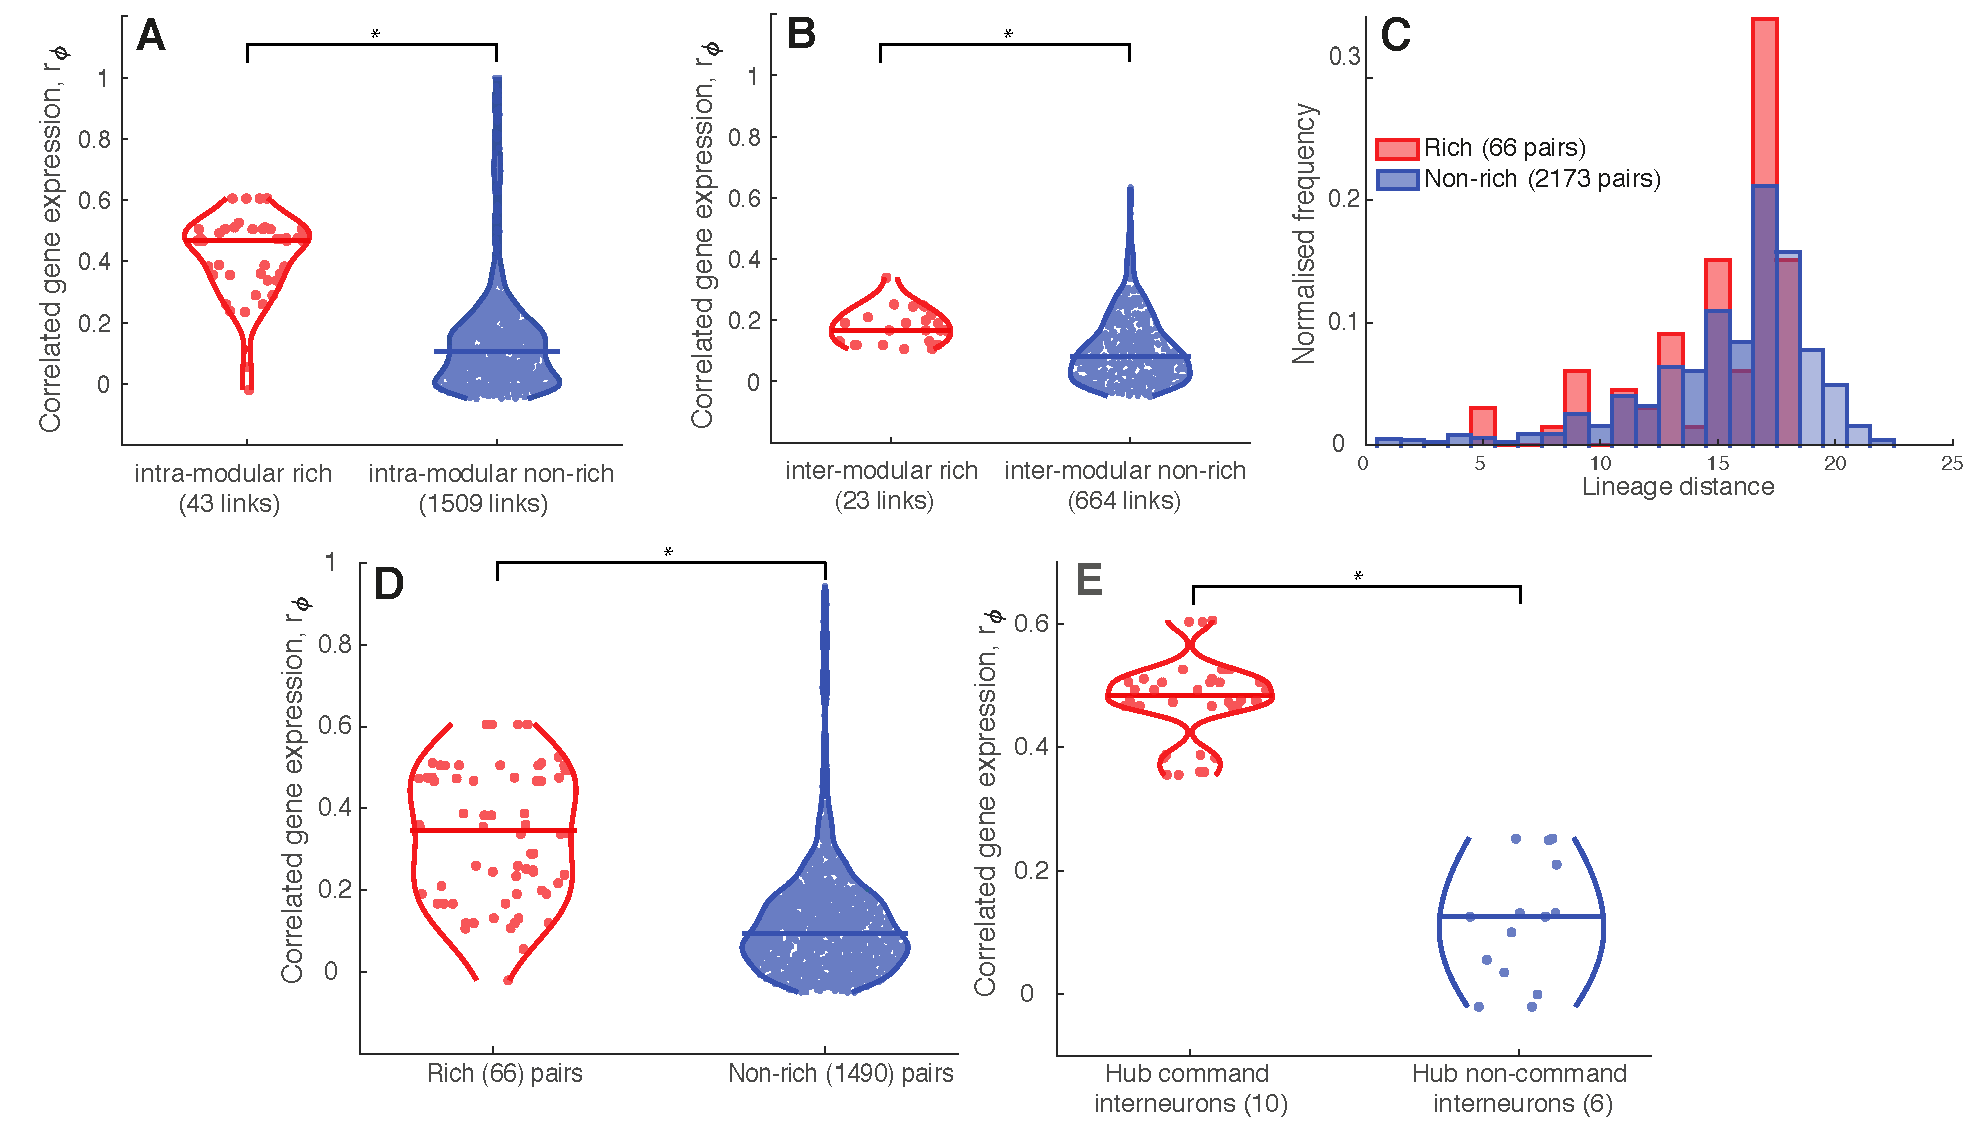
\includegraphics[width=1\textwidth]{extrasALL2.pdf}
 \caption{
 \textbf{Increased CGE of hub neurons is not driven by modularity, neuronal birth time, or cell lineage distance.}
%\textbf{A: Connection distance}
%Top: Degree distribution.
%Bottom: Median lineage distance for rich, feeder, and peripheral connections as a function of \textit{k}, with the %median across all network links shown as a dashed black line and the topological rich club regime shaded grey.
%Circles indicate a statistically significant change in lineage distance in a given link type relative to the rest %of the network (Wilcoxon rank sum test; $p < 0.05$). \\
%\textbf{A} Nematode connectivity matrix organized by topological module (white squares), with all connections labeled by type: rich (red), feed-in (yellow), feed-out (orange), and peripheral (blue).
%Neuron indicators are shown to the left:
%(i) module assignment,
%(ii) neuron type (interneuron, orange; motor, green; sensory, blue; multimodal, yellow),
%(iii) hub indicator (red for hubs), and
%(iv) spatial position: head (gray), body (purple), tail (red).
(A) Distributions of CGE, $r_\phi$, for intra-modular rich (red) non-rich (blue) connections, shown as violin plots with the median shown as a horizontal bar (Wilcoxon rank sum test, $p = 6.9 \times 10^{-17}$).
% The number of connections of each type is shown in parentheses.
(B) Distributions of CGE, $r_\phi$, for inter-modular rich (red) and non-rich (blue) connections, shown as violin plots with the median shown as a horizontal bar (Wilcoxon rank sum test, $p = 1.6 \times 10^{-5}$).
% The number of connections of each type is shown in parentheses.
(C) Distributions of lineage distance between rich links (red) and non-rich links (blue), plotted as histograms due to a discrete nature of this measure (Wilcoxon rank sum test, $p = 0.079$).
(D) Distributions of CGE, $r_\phi$, between early born hubs (rich links, red) and nonhubs (non-rich links, blue) shown as violin plots with the median shown as a horizontal bar (Wilcoxon rank sum test, $p = 3.9 \times 10^{-22}$).
(E) Distributions of CGE between hub command interneurons (red) and hub non-command interneurons (blue) shown as violin plots with the median shown as a horizontal bar (Wilcoxon rank sum test, $p = 3.3 \times 10^{-8}$). * represents statistically significant differences.
%[[TODO: could add neurotransmitter type as a bar code in modules]]
%[[TODO: change colors for distributions, fill distributions, e.g., intra-modular and inter-modular shouldn't use red (rich) use green for non-rich]]
%Composition of each module according to neuron type.
%Modular organisation of the connectome.
%Coexpression distributions within and between modules.
%\textbf{C: Lineage distance}
%Top: Degree distribution. Bottom: Mean lineage distance for rich, feeder, and peripheral connections as a function %of \textit{k}, with the median across all network links shown as a dashed black line and the topological rich club regime shaded grey.
%Circles indicate a statistically significant change in lineage distance in a given link type relative to the rest of the network (one-sided Welch’s t-test; $p < 0.05$) \\
%\textbf{D: Coexpression for different types of neurons. }
%Top: Median CGE as a function of degree for connections involving different types of neurons.
%Bottom: The number of connections in each category for a range of degrees.
%Coexpression distributions for hub and nonhub interneurons.\\
}
 \label{fig:Fig8}
\end{figure}

\paragraph{Lineage distance.}
%[[should first characterize general relationship between lineage and CGE, and then address hub effect]] -- there is no general lineage-CGE effect in our results.
The lineage distance between a pair of neurons is defined as the sum of total divisions that have taken place since the most recent common ancestor cell \cite{Pavlovic:2014gx, Sulston1977, Sulston1983}.
In the mammalian brain, neuronal lineage has been associated with both functional properties \cite{Ciceri2013, Li2012} as well as connectivity \cite{Yu2012}.
Moreover, tissue distance (resembling lineage distance on a cellular scale) correlates with gene expression divergence, meaning that tissues from the same branch on the fate map share more similar gene expression patterns in both human and mouse mesoderm as well as ectoderm tissues \cite{Cui2007}.
Given that the ectoderm eventually differentiates to form the nervous system, this finding suggests a possible relationship between lineage distance and CGE in a microscale neuronal system such as that of \textit{C. elegans}.
%Therefore, lineage distance could potentially be an informative source of information about the genetic makeup of the \textit{C. elegans} nervous system \cite{Schroter:2017eo}.
However, we find no significant correlation between lineage distance and CGE in \textit{C. elegans} (Spearman's $\rho = -0.027$, $p = 0.2$).
As shown in Fig.~\ref{fig:Fig8}C, there was only a weak tendency for the meadian lineage distance lineage distance to be increased in non-rich pairs (Wilcoxon rank sum test, $p = 0.079$).
%[[Could do as pairs rather than connected...? - THERE IS A sign DIFFERENCE if we take all pairs instead of connections - hubs are more close in lineage it means that there are no connections between hubs that are closest in lineage, while literature suggests, that some neurons in mouse form connections preferentially with `sister' neurons as in Yu, 2012.]].
%all hub neurons are formed early in development as characterized above, and hence it is possible that they originate from common ancestry cells and share intrinsic similarities in gene expression that influence the observed increase in CGE between hub neurons.
%It may be the case, for example, that hub neurons are derived from similar cell lines, which may drive their increased CGE.
Thus, we can not attribute the transcriptional similarity of connected hub neurons to their neuronal lineage.


\paragraph{Birth time.}
The genesis of neurons in \emph{C. elegans} is separated into two distinct time periods: before hatching (birth time $<550$ min -- `early-born') and after hatching (birth time $>1200$ min -- `late-born'), with no neurons formed during intermediate times \cite{Varier2011}.
%Distinguishing neurons into these two groups is appropriate as birth time differences between pairs of neurons are dominated by the difference between these two clusters of neuron birth periods.
As a broad group, connected pairs of early-born neurons do not exhibit significantly different CGE compared to connected pairs of late-born neurons (Wilcoxon rank sum test, $p = 0.64$), but connected pairs of early-born neurons do exhibit significantly higher CGE relative to pairs of connected neurons for which one neuron is born prior to hatching and the other is born after hatching (Wilcoxon rank sum test, $p = 4.2 \times 10^{-3}$).
Since all \emph{C. elegans} hub neurons are born prior to hatching \cite{Towlson2013} and neurons born at similar times may share similar connectivity properties \cite{Varier2011, Towlson2013}, we investigated whether the increase in CGE between hub neurons of \emph{C. elegans} may be driven by their similar birth times.
% , we investigated whether  hub neurons is influenced by their early birth times.
% they exhibit significantly higher CGE comparing to connections that exist between those two neuron groups.
% with an around 700min gap between them when no neurons are formed.
% \cite{Varier2011, Towlson2013}.
Focusing on the 201 neurons born prior to hatching (16 hub and 185 nonhub neurons), connected pairs of hub neurons exhibit significantly increased CGE, $r_\phi$, relative to other pairs of connected early-born neurons (Wilcoxon rank sum test, $p < 10^{-22}$), as shown in Fig.~\ref{fig:Fig8}D.
% i.e., feed-in, feed-out, and peripheral connections - non-rich links;
 % to see whether connections between hub neurons displayed increased CGE relative to other types of connections between neurons born during this early developmental phase.
% Hub neurons are thus distinctively similar in their expression patterns, even amongst early-born neurons.
% We conclude that the increased CGE between hub neurons is not driven by the similarity in their birth times.

% Adj = GiveMeAdj(C,'zeroBinary','ch');k = sum(Adj) + sum(Adj,2)';
% sum(C.BirthTime<550 & k>41) = 13
% sum(C.BirthTime<550 & k<=41) = 188

%[[not sure this is relevant/fits the story. Could remove:]]\\
%Looking closer, we find that lineage distance increases with degree for feeder links while no significant change is observed for rich links (Fig.~\ref{fig:Lineagek}).
%This finding suggests that neurons forming peripheral links are most similar in lineage nonhub-hub connected pairs have significantly increased lineage distance (Fig.~\ref{fig:Lineagek}).

%hub and nonhub neurons have a higher lineage distance for high thresholds of $k$, i.e., when so-called hubs actually have high degree.
%In contrast, peripheral links manifest consistently lower lineage distance through the range of degree thresholds (Fig.~\ref{fig:Lineagek}).


%peripheral are most similar in lineage and interesting, feeder the most different, implying that nonhub-hub connected pairs have significantly increased lineage distance.

\paragraph{Neurochemistry.}
% <<TypeConfoundHubs.m>>
Hub neurons ($k > 44$) consist of thirteen cholinergic neurons, two glutamatergic neurons, and one neuron of unknown neurotransmitter type \cite{Pereira:2015er}.
We find that neuron pairs show different CGE relationships as a function of their neurotransmitter type, e.g., pairs of GABAergic neurons have high median CGE, $\tilde{r}_\phi = 0.59$, while pairs of glutamatergic neurons exhibit a relatively low median CGE, $\tilde{r}_\phi = 0.08$.
% TypeConfoundHubs.m
To determine whether the similarity in CGE between pairs of hub neurons could be explained by their neurotransmitter types, we constructed $10^8$ random sets of sixteen neurons of the same neurotransmitter types as hubs (e.g., thirteen random cholinergic neurons, two random glutamatergic neurons, and one random neuron of an unknown neurotransmitter type) and compared the distribution of median CGE of each group to the median CGE of hub neurons as a permutation test.
Neurochemical identity cannot explain the elevated CGE of hub neurons, with hubs displaying a significant increase in median CGE relative to random sets of neurons with the same neurotransmitter types as hubs (permutation test, $p = 2.57\times10^{-6}$).
% used a permutation test, computing the median CGE between random groups of  across $1\times 10^6$ permutations.
% The mean CGE between hub neurons is significantly increased relative to random sets of neurons with the same neurotransmitter types as hubs (permutation test, $p = 3.2\times 10^{-5}$).
% The increased CGE between hub neurons cannot be explained by their neurotransmitter identities, with hub neurons displaying

\paragraph{Anatomical location.}
% <<TypeConfoundHubs.m>>
Of the sixteen hub neurons, thirteen are in the head and three are in the tail; none are located in the body.
CGE varies as a function of anatomical location (i.e., `head', `body', and `tail'), with pairs of neurons in the same anatomical class exhibiting the highest median CGE (e.g., pairs of neurons within the body have a median $\tilde{r}_\phi = 0.14$, pairs of neurons within the tail have $\tilde{r}_\phi = 0.12$, and pairs of neurons within the head have $\tilde{r}_\phi = 0.07$), followed by lower median CGE in mixed classes (e.g., head-body pairs of neurons have $\tilde{r}_\phi = 0.01$).
Given this variation, we tested whether the increased CGE between hub neurons could be explained by their anatomical distribution using the permutation testing procedure described above for neurochemistry.
That is, we compared the distribution of CGE between hubs to a null distribution formed from $10^8$ random permutations of thirteen head neurons and three tail neurons.
% TypeConfoundHubs -> doWhat='anatomy'
The median CGE, $\tilde{r}_\phi$, between hub neurons is significantly increased relative to random sets of thirteen head neurons and three tail neurons (permutation test, $p = 2.62\times10^{-6}$).
Furthermore, CGE is significantly increased amongst hub neurons relative to other pairs of head neurons (Wilcoxon rank sum test, $p = 4.1 \times 10^{-11}$ for 46 hub-hub pairs and 1\,186 others),
and also amongst head/tail pairs of neurons (Wilcoxon rank sum test, $p = 1.6 \times 10^{-14}$ for 23 hub-hub pairs, 174 others),
but not for the three hub neurons in the tail (Wilcoxon rank sum test, $p = 0.15$ for three hub-hub pairs, 53 others).
Thus, anatomical location cannot explain the high CGE of hub neurons.

\paragraph{Functional class.}
\emph{C. elegans} neurons can be divided into distinct groups that each perform a specialized behavioral function \cite{Hobert2003}.
One of the best-characterised functional classes that is particularly relevant for our analysis is the set of `command interneurons' which are a functional group of ten neurons that govern forward (AVBL, AVBR, PVCL, PVCR) and backward (AVAL, AVAR, AVDL, AVDR, AVEL, AVER) locomotion \cite{Rakowski2013}.
All of these neurons are hubs.
% ten out of sixteen hub neurons correspond to the functional circuit that governs forward (AVBL, AVBR, PVCL, PVCR) and backward (AVAL, AVAR, AVDL, AVDR, AVEL, AVER) locomotion, which are together known as `command interneurons' [[REF]].
Given the overlap between hub neurons and command interneurons, we investigated whether command interneurons exhibit more similar expression than other hub interneurons, and may therefore drive the increase in CGE amongst hubs as a whole.
We compared CGE, $r_\phi$, between all pairs of command interneurons (ten neurons), and between all pairs of hubs that are not command interneurons (six neurons), shown in Fig.~\ref{fig:Fig8}E.
Correlated gene expression between command interneurons is significantly greater than between other hub neurons (Wilcoxon rank sum test, $p = 3.3 \times 10^{-8}$), indicating that command interneurons play a major role in driving the increased CGE amongst hub neurons.
Moreover, there is no difference in CGE between pairs of hubs that are not command interneurons (DVA, RIBL, RIBR, AIBR, RIGL, AVKL) and a set of seven anatomically matched nonhub head interneurons (AVFL, AVFR, AVHL, AVHR, AVJL, AVJR, AVKR) (Wilcoxon rank sum test, $p = 0.13$), indicating that the status of many hub neurons as command interneurons makes a significant contribution to the elevated CGE of hubs.

%Relative to macroscopic brains in which hubs are often distributed across diverse neural systems \cite{Fulcher:2016ck}, it is not possible to disentangle the role of specialized functional circuits from connectivity in \emph{C. elegans}, with highly connected hubs containing the transcriptionally uniform set of command interneurons.


\subsection*{Genes driving correlated gene expression patterns}
%% comment on enrichment analysis. No write up can be done before deciding on options.
% Having determined that pairs of neurons with different connectivity exhibit different levels of CGE,
Having characterized a robust relationship between CGE and (i) connectivity, and (ii) hub connectivity, we next investigated which specific genes contribute most to this relationship.
Despite challenges with the incomplete binary expression measurements in a small proportion of the genome, we developed a method to score genes according to their contribution to a given CGE pattern (see \emph{Methods}).
We characterized individual high-scoring genes, with $p_\mathrm{corr} < 10^{-4}$ (approximately 20\% of genes with the highest scores in each analysis), and attempted to summarize functional groups of genes as biological process categories of the gene ontology (GO) that were enriched in high scoring genes using overrepresentation analysis (ORA) \cite{Ashburner2000, Gillis2010}.

We first investigated which genes drive increased CGE in connected pairs of neurons relative to unconnected pairs.
Previous studies in mouse have indicated that genes driving an increase in CGE between connected pairs of brain regions are enriched in GO categories related to neuronal connectivity and communication \cite{Fulcher:2016ck, Ji:2014jw, Fakhry:2015kl, French2011}.
First, we manually investigated individual high-scoring genes (i.e., those with $p_\mathrm{corr} < 10^{-4}$, see Supplementary Data File, \textbf{GeneList.xlsx}).
% submitted to ORA analysis
Given that glutamate is a prevalent neurotransmitter in \textit{C. elegans} (26\% of neurons with known neurotransmitter type are glutamatergic \cite{Pereira:2015er}), it is appropriate that many high scoring genes are related to glutamate receptors (including \emph{glr-1}, \emph{glr-2}, \emph{glr-4}, \emph{glr-5}, \emph{nmr-1}, and \emph{nmr-2}).
Consistent with the importance of innexins in forming electrical synapses \cite{Starich2001}, our list contained the following innexin genes: \emph{unc-9}, \emph{unc-7}, \emph{inx-7}, \emph{inx-19}, \emph{inx-13}.
% the involvement of both neurotransmitter as well as electrical synapse related genes is expected.
% innexins .
% cell adhesion molecules, and transcription factors were found.
Genes encoding cell adhesion molecules related to axon outgrowth and guidance, cell migration and locomotion (\emph{sax-3}, \emph{cam-1}, \emph{unc-6}, \emph{rig-1}, \emph{unc-5}), learning (\emph{casy-1}) \cite{Zallen1999, Garriga1999, Leung-Hagesteijn1992, Harris:2009kd, Ikeda2008},
as well as genes involved in determining cell polarity (\emph{vang-1}, \emph{prkl-1}) \cite{Wu2006, Hoffmann2010} were also amongst the top scoring genes for connectivity.
These genes have been implicated in neuronal connectivity in both flies and humans \cite{Paemka2013, Ehaideb2016, Sowers2013}, with our results predicting that they may play a similar role in \textit{C. elegans}.
In addition, transcription factors regulating neuronal development,
fate specification (\emph{lin-11}, \emph{unc-3}, \emph{unc-42}, \emph{ceh-14}, \emph{ast-1}, \emph{cfi-1}) \cite{Sarafi-Reinach2001, Prasad2008, Baran1999, Cassata2000, Schmid2006, Shaham2002a},
and locomotion (\emph{unc-3}) \cite{Prasad2008}) were also implicated in driving increased CGE amongst connected pairs of neurons.
Both adhesion molecules and transcription factors are candidates for facilitating signal transduction and communication.

In order to summarize the above mentioned results and determine if any particular functional groups of genes are dominating in driving this effect, we performed an enrichment analysis.
Top scoring biological process GO categories from ORA analysis (of 85 genes relative to the 414 genes with sufficient data for this analysis) are listed in \nameref{tab:enrichmentCON}.
Although no GO categories are significant at a false discovery rate of 0.05, the top categories are consistent with a connectivity profile, including `glutamate receptor signaling', `cell surface receptor signaling', and `ion transport', with other categories involved in regulation of growth rate and several related to catabolic processes.
Thus, despite incomplete gene expression data that do not provide sufficient coverage to detect statistically significant effects, these results indicate that our data-driven gene scoring method is able to yield sensible, biologically relevant insights into the genetic basis of neuronal connectivity in \textit{C. elegans} connectome.

% (related to the probability of a gene being expressed together in a given set of neuron pairs compared to an alternative set).
%Relative to previous work in mouse, for example \cite{Fulcher:2016ck, Ji:2014jw, Fakhry:2015kl, French:2011cz}, the current data are more challenging due to incomplete binary expression measurements in a small proportion of the genome.
%Here we also show that adhesion molecule genes related to axon outgrowth and guidance (sax-3 \cite{Zallen1999}, cam-1 \cite{Garriga1999}), cell migration (cam-1 \cite{Garriga1999}, unc-6, rig-1, unc-5 \cite{Leung-Hagesteijn1992}), locomotion (cam-1, unc-5 \cite{Harris:2009kd}), learning (casy-1 \cite{Ikeda2008}) as well as two orthologs of Drosdophila genes involved in determining cell polarity (vang-1 \cite{Hoffmann2010}, prkl-1 \cite{Wu2006}) are implicated.
%In addition, transcription factors regulating neuronal development, fate specification (lin-11 \cite{Sarafi-Reinach2001}, unc-3 \cite{Prasad2008}, unc-42 \cite{Baran1999}, ceh-14 \cite{Cassata2000}, ast-1 \cite{Schmid2006}, cfi-1 \cite{Shaham2002a}) and locomotion (unc-3 \cite{Prasad2008}) also play an important role in the increased CGE between connected neurons. \\
%regulating cell interaction with the surface or other cells, therefore potentially facilitate signal transduction and communication,
%While these incomplete binary expression data do not allow us to deduce functional categories with statistical significance, our findings point to the possible role of some relevant neuronal processes in driving the increased CGE of connected pairs of neurons relative to unconnected pairs.
 % demonstrate a method for computing GO categories from binary expression data that suggest that connected pairs of neurons may coexpress genes associated with neuronal connectivity relative to unconnected neuron pairs.
Having characterized genes that contribute to the increase in CGE between connected pairs of neurons, we next investigated whether particular functional groups of genes drive differences in CGE between connections involving hub neurons (i.e., in rich, feed-in, and feed-out connections) relative to connections between pairs of nonhub neurons (i.e., peripheral connections).
%Our inability to get a comprehensive understanding of neurotransmitter signaling for the gene expression data used here is related to its incompleteness, e.g., only one acetylcholine-related GO category---`synaptic transmission, cholinergic' (GO:0007271)---contained sufficiently many genes (fourteen) to be represented in our enrichment analysis.
% [[DO WE SHOW NUMBER IN DATA OR IN GENE SETS USED FOR CON and RF analysis]] while others (n=9) had only up to 3 genes, therefore were not included in the enrichment analysis as categories with 5-100 genes were required.
%Glutamate release categories were also not represented here (each were annotated with fewer than five genes in our dataset and hence excluded).
% including `positive regulation of biosynthetic process', two groups responsible for positive regulation of nitrogen and nucleobase-containing compound metabolic process, `positive regulation of cellular metabolic process', and `positive regulation of macromolecule biosynthetic process'.
In order to investigate which specific genes contribute most to the increase in CGE for connections involving hubs, we first investigated the highest-scoring genes, with $p_\mathrm{corr} < 10^{-4}$ (corresponding to approximately the top 20\% of genes in the analysis).
In addition to glutamate receptor genes (\emph{glr-5}, \emph{nmr-1}, \emph{nmr-2}, \emph{glr-1}, \emph{glr-2}, \emph{grld-1})
and acetylcholine related genes (\emph{ace-2}, \emph{cho-1}, \emph{unc-17}, \emph{deg-3}),
we again find a high number of genes regulating cell adhesion (\emph{cam-1}, \emph{rig-1}, \emph{rig-6}, \emph{unc-6}, \emph{grld-1}, \emph{dbl-1}, \emph{ncam-1})
and relevant transcription factors (\emph{unc-3}, \emph{unc-42}, \emph{ast-1}).
% that at least partially overlap with genes found comparing connected and unconnected pairs of neurons.
The implication of glutamate and acetylcholine may be attributable to the importance of glutamate in the regulation of locomotion in command interneurons \cite{Choi2015, Zheng1999}, with acetylcholine being the dominant neurotransmitter in hubs (13 out of 16 hubs are cholinergic).
We also find a high overlap between adhesion molecule and transcription factor genes found in the previous analysis and the implication of human orthologs (\emph{rig-1}, \emph{ncam-1}, \emph{grld-1}, corresponding to human genes ROBO4, NCAM2, and RBM15 respectively  \cite{Harris:2009kd}) for genes regulating cell migration, differentiation and neuron cell adhesion.

% ---also emerged as enriched in connections involving hubs compared to other connections.
%These findings are in line with our expectations as hub neurons receive input from sensory neurons, the majority of which are glutamatergic.
%As a result, hubs are required to have glutamate receptors the enrichment in these categories is the most pronounced (even after the correction, false discovery rate $< 0.05$).
%[[AA: part about glutamate and Ach should probably be excluded according to Alex's comment or we can keep it if we put a list of top genes - plenty of locomotion and glutamate there.]].
%The implication of glutamate receptor signaling for synaptic connectivity, and hub connectivity in particular, is somewhat surprising given that only 26\% of neurons with known neurotransmitter type are glutamatergic (whereas 55\% are cholinergic) and just two of the sixteen hubs are glutamatergic (thirteen are cholinergic, and one is of unknown type).
%Furthermore, just 32\% of neurons that project to hubs are glutamatergic.
% FeedInOutNodes;

While previous work implicated genes regulating oxidative metabolism for connections involving hubs in mouse \cite{Fulcher:2016ck}, and for hub regions in human \cite{Vertes2016a}, the gene expression dataset used here was not sufficiently comprehensive to investigate these processes.
For example, only one of the 948 genes annotated to the GO categories related to hub connectivity in mouse is present in our gene expression dataset (\emph{unc-32} is annotated to the GO category: `ATP hydrolysis coupled proton transport').
% GO:0015991:
% GO categories were filtered using <<searchGOcategories.m>> function.
Thus, although a direct test of the metabolic hypothesis for neural hubs is not possible from current data, we investigated whether other biological process GO categories were overrepresented in pairs of connected hubs using ORA (of 30 genes relative to the 168 genes with sufficient data for this analysis), with results listed in \nameref{tab:enrichmentRICH}.
% , providing some support for the idea that hubs are energetically costly elements of the connectome.
%Due to gene expression data specificity in all the following analyses we present top 15 GO categories enriched in a particular link type compared to other links.
Even though no categories are statistically significant at a false discovery rate of 0.05, the list of top categories includes both `glutamate receptor signaling pathway' as well as more general `cell surface receptor signaling pathway' in addition to several ion transport related gene groups ('ion transport', `ion transmembrane transport', `transmembrane transport').
Other top-ranked GO categories include regulation of locomotion, and various metabolism and biosynthesis related processes.
Our gene scoring method again yields interpretable insights into the types of genes that contribute to differences in CGE between different classes of neuronal connections in \emph{C. elegans}.
While current data are limited, more comprehensive expression annotations in the future would allow more systematic and statistically powered inferences across GO categories.
% , thus were not included in the analysis.
%% [GenesinGO, GOs] = searchGOcategories(C,G,'glutamat');
%% [GenesinGO, GOs] = searchGOcategories(C,G,'cholin');

% [k,sortedLabels] = NeurotransmitterAnal(C,false); mean(sortedLabels(sortedLabels~='Unknown (orphan)')=='ACh')
% we found enrichment in glutamate receptor signaling when comparing connections between hubs to those not involving hubs.
% with ACh being the most broadly used neurotransmitter in general \cite{Pereira:2015er}
% It is worth noting that although both analyses above highlighted enrichment of glutamate, even though acetylcholine (ACh) is the most broadly used neurotransmitter in \textit{C. elegans} \cite{Pereira:2015er}, and most hubs ($k > 41$) are cholinergic (Fig.~\ref{fig:S_feedInOutNodes}C).
% [[WILL EXCLUDE THAT AS NOW MOST FEEDERS ARE BOTH IN AND OUT, numbers updated but picture not]] \\
% Looking closer at the neurotransmitter type of each neuron, we found that nonhub neurons that project to hubs (but do not receive projections back) are mostly sensory or interneurons (74\%), with the most common neurotransmitter being glutamate (32\%), whereas neurons that receive inputs from hubs (but do not project to hubs) are mostly motor neurons (75\%) and are cholinergic (67\%), as shown in Fig.~\ref{fig:S_feedInOutNodes}A,C.\\

% but our findings imply that Glu drives \emph{coupled} expression, so Glu genes are being expressed in both neurons, not just one, implying that that the presynpatic neuron expresses genes associated with Glu synthesis and the post-synaptic neuron (hub) expresses Glu receptor genes.

%Are presynaptic genes represented in the Glu pathway GO category?

% [[Thus, although hubs are themselves mostly cholinergic, they receive inputs from glutamatergic neurons, which may explain the enrichment of the two GO biological process categories related to glutamate receptors.
% PROBABLY INCLUDE SOME POSSIBLE EXPLANATION without hard numbers as now almost all feeder links are feed-both IN DISCUSSION, not HERE]].

% Although we were unable to test the hypothesis proposed in the previous work in mouse connectome \cite{Fulcher2016}, several metabolism and biosynthesis related categories enriched in connections involving hubs allow us to draw some parallels and reaffirm that hub connectivity on a neuronal scale might also be [[IS?]] experience increased energy demands.
% : `ionotropic glutamate receptor signaling pathway' and `glutamate receptor signaling pathway'.

%[[MAY NOT BE NECESSARY:]] NO CLEAR STORY WITH NEW ENRICHMENT RESULTS, probably should exclude it.
%To disentangle differences between projections to and from hubs by nonhubs, we performed an enrichment analysis separately for feed-in and feed-out connections, expecting enrichment in cholinergic signaling for feed-out links that involve projections from cholinergic hub neurons, and glutamate signaling for feed-in links.
%Results are shown in Table~\ref{enrichmentFeedIN} and Table~\ref{enrichmentFeedOUT} for feed-in and feed-out connections, respectively.
%The list of top categories for both connection types contained `neurotransmitter metabolic process', and `synaptic transmission, cholinergic'.

% Both feed-in and feed-out links were enriched in chemical transmission, metabolism and cholinergic synaptic transmission related genes (see Table.~\ref{enrichmentFeedIN} and \ref{enrichmentFeedOUT})).


% This may explain the overrepresentation of glutamate receptor related categories that we find in the enrichment analysis.

%\begin{figure}[h]
%\centering
 %   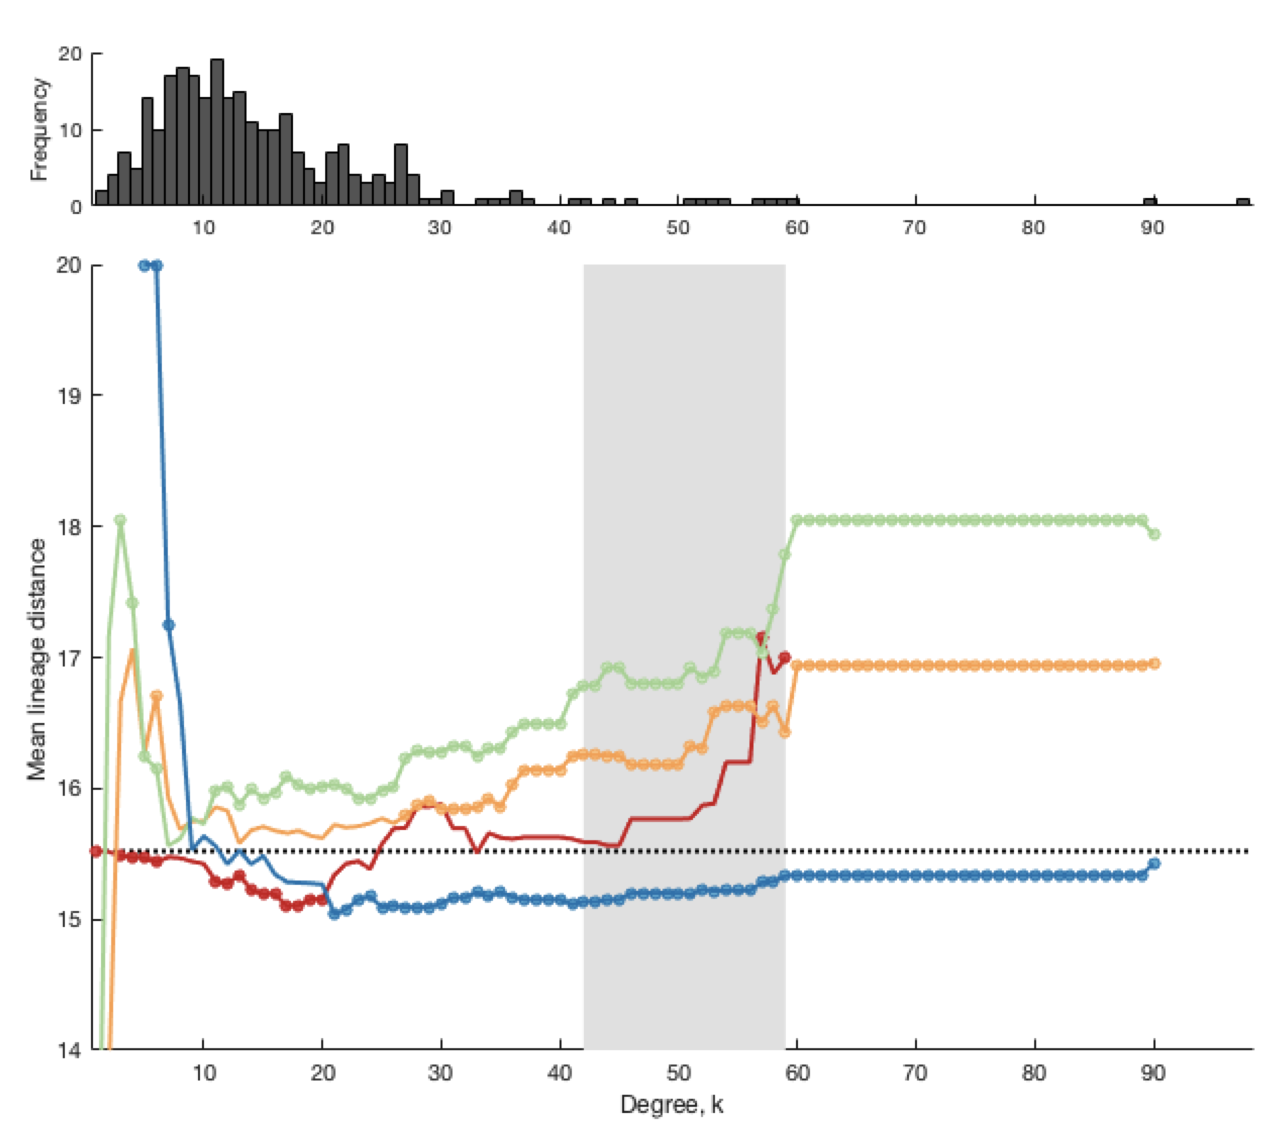
\includegraphics[width=0.7\textwidth]{LineageRFP}
 %\caption{\textbf{}
 %\label{Lineage}
 %\end{figure}

% Place tables after the first paragraph in which they are cited.
% \begin{table}[!ht]
% \begin{adjustwidth}{-2.25in}{0in} % Comment out/remove adjustwidth environment if table fits in text column.
% \centering
% \caption{
% {\bf Table caption Nulla mi mi, venenatis sed ipsum varius, volutpat euismod diam.}}
% \begin{tabular}{|l+l|l|l|l|l|l|l|}
% \hline
% \multicolumn{4}{|l|}{\bf Heading1} & \multicolumn{4}{|l|}{\bf Heading2}\\ \thickhline
% $cell1 row1$ & cell2 row 1 & cell3 row 1 & cell4 row 1 & cell5 row 1 & cell6 row 1 & cell7 row 1 & cell8 row 1\\ \hline
% $cell1 row2$ & cell2 row 2 & cell3 row 2 & cell4 row 2 & cell5 row 2 & cell6 row 2 & cell7 row 2 & cell8 row 2\\ \hline
% $cell1 row3$ & cell2 row 3 & cell3 row 3 & cell4 row 3 & cell5 row 3 & cell6 row 3 & cell7 row 3 & cell8 row 3\\ \hline
% \end{tabular}
% \begin{flushleft} Table notes Phasellus venenatis, tortor nec vestibulum mattis, massa tortor interdum felis, nec pellentesque metus tortor nec nisl. Ut ornare mauris tellus, vel dapibus arcu suscipit sed.
% \end{flushleft}
% \label{table1}
% \end{adjustwidth}
% \end{table}


%PLOS does not support heading levels beyond the 3rd (no 4th level headings).

% \subsubsection*{3rd level heading}
% Text.
%
% \begin{enumerate}
%     \item{react}
%     \item{diffuse free particles}
%     \item{increment time by dt and go to 1}
% \end{enumerate}
%
%
% \subsection*{Another subsection}
%
%
% \begin{itemize}
%     \item First bulleted item.
%     \item Second bulleted item.
%     \item Third bulleted item.
% \end{itemize}

\section*{Discussion}
Highly connected hubs of neural systems play an important role in brain function, with their dense rich-club interconnectivity integrating disparate neural networks \cite{vandenHeuvel:2013ge, Fornito2015, deReus:2013cy, vandenHeuvel:2013ij}.
Here, our analysis linking hub connectivity of the microscale connectome of \emph{C. elegans} to patterns of neuron-specific gene expression has identified a transcriptional signature that appears to be highly conserved, given recent findings reported in a mesoscale investigation of the mouse \cite{Fulcher:2016ck} and a macroscale study of humans \cite{Vertes2016a}.
Specifically, we show that:
(i) CGE is higher for connected pairs of neurons compared to unconnnected pairs;
(ii) the neuron connection probability decays as a function of spatial separation, and;
% and similarity of gene expression
(iii) connected pairs of hub neurons, which are generally separated by longer anatomical distances, show the highest levels of CGE.
% counter this general trend by
This association between CGE and hub connectivity followed a gradient, such that CGE was lowest for connected nonhubs, intermediate for hub-nonhub pairs, and highest for connected hubs, consistent with results reported in the mouse brain \cite{Fulcher:2016ck}.
% Our results cannot be attributed to the fact that hub neurons are interneurons, are born prior to hatching, are more likely to be in the same network module, are mostly cholinergic, are mostly in the head, or to the lineage similarity of hub neurons.
% However, given the overlap between hub neurons with functional class of command interneurons, we are unable to discount the possibility that these command interneurons drive the high CGE between hub neurons in \emph{C. elegans}.
Amongst the genes considered here, many of those with the greatest contribution to connectivity are biologically plausible genes related to receptors, neurotransmitters, and cell adhesion, and those with the greatest contribution to hub connectivity are related to glutamate receptors, acetylcholine signaling, and other neuronal communication related genes.
The methods we develop here for quantifying CGE, and for scoring the contribution of individuals genes to overall CGE, yield biologically interpretable results from incomplete binary gene expression data.
With improvements in gene annotation quality and specificity, and increases in genome coverage, similar methods could be used in future work to characterize the biological basis of a range of neuronal connectivity patterns.

% Introduce gene expression work in C elegans(Kaufman) and prior work relating gene expression and connectivity (mouse, human)}
%The recent availability of gene expression data in the brain has allowed structural connectome properties to be related to molecular information \cite{vandenHeuvel:2017ex}, facilitating cross-scale understanding between the fields of macroscale connectomics and microscale neuroscience \cite{vandenHeuvel:2017ex}.
%Initial statistical work done using binary gene expression annotations in \emph{C. elegans} showed that the expression of a small number of genes can be used to predict connectivity between pairs of neurons \cite{Varadan:2006ek, Kaufman2006, Baruch2008b}.
%Later work, utilizing detailed quantitative gene expression data in mouse from the Allen Mouse Brain Atlas \cite{Lein:2007jn} revealed a relationship between gene expression and connectivity in mouse \cite{Ji:2014jw, Fakhry:2015kl}, with pairs of brain regions with similar gene expression patterns also displaying similar connectivity profiles (using connectivity data from rat) \cite{French2011}.\\
%Comparing different types of connections in mouse, we have demonstrated that pairs of connected hubs have the most similar gene expression profiles, and that hub connectivity is associated with the correlated expression of genes related to oxidative energy metabolism \cite{Fulcher:2016ck}.
%Similar findings have been reported at the regional level in the human cortex, with integrative hub regions (with high inter-modular degree and long connection distance) being associated with expression of genes regulating oxidative metabolism and mitochondria \cite{Vertes2016a}.
%Both results are consistent with the high metabolic cost of hubs \cite{Collin:2014kq, Tomasi:2013kl}, which may be due to the high signal traffic they're thought to mediate \cite{vandenHeuvel:2012kh, Misic:2014it}, painting a picture of hubs as a highly conserved and metabolically costly feature of structural brain networks.

%These findings highlight a close relationship between metabolic expenditure and the high signaling load of hub regions in the brain, as has been previously proposed \cite{Bullmore2012}.
%As well as being a highly conserved structural feature, these studies hint that hub connectivity may also be consistently related to metabolic demand, with the picture of highly connected hubs being both metabolically costly, both to construct and to run.

It is reasonable to expect that the principles of neural organization may differ from the scale of individual neurons to the scale of macroscopic brain regions (in which each brain region contains millions of neurons).
However, many of our results in \emph{C. elegans} suggest a striking conservation of many fundamental spatial trends in neural connectivity and CGE across scales and species.
For example, connection probability decreases with spatial separation between brain areas in rodents and primates \cite{Horvat:2016ia, Wang:2016gg} (including in macaque \cite{Markov:2013jo}, human \cite{Henderson:2014fg}, mouse \cite{Fulcher:2016ck}, and rat \cite{Noori:2017ce}),
for individual neurons in mouse primary auditory cortex \cite{Levy:2012dy},
and between neurons in \emph{C. elegans} (cf. Fig.~S1 of \cite{Azulay:2016cg}).
% Previous results have from the scale of individual neurons in mouse primary auditory cortex \cite{Levy:2012dy} to the scale of macroscopic brain regions \cite{Fulcher:2016ck}.
Unlike mammalian brains, where all neurons are confined to a spatially contiguous organ, neurons are distributed across nearly the entire length of \emph{C. elegans}, including a dense cluster of neurons in the head and in the tail.
Despite these distinct morphologies, we report a qualitatively similar spatial dependence of connection probability with separation distance for many classes of connections in \emph{C. elegans}, including those within the head, body, and tail, indicating that this distance-dependence may be a generic property of evolved neuronal systems that must balance the energetic cost of long-range connections with their functional benefit \cite{Bullmore:2012vl, vandenHeuvel:2012kh, Kim:2014bu, Betzel:2016jt}.
Less frequently characterized is the spatial dependence of CGE, with available evidence indicating that more proximal brain areas exhibit more similar gene expression patterns than more distant brain areas in the mouse brain \cite{Fulcher:2016ck} and human cortex \cite{Krienen:2016eq, Pantazatos:2016ir, Richiardi:2017hb}.
Some of the spatial trends in CGE found in the 948 genes analyzed here mirror these trends of bulk regions of macroscopic mammalian brains.
It is therefore possible that these spatial dependences of connectivity and CGE may not be simply due to bulk spatial trends in macroscopic brains containing millions of neurons, but may reflect conserved organizational principles that hold across species and spatial scales.
Our results highlight the importance of treating nervous systems as spatially embedded objects, as many seemingly non-trivial properties of brain organization may be well approximated by simple, isotropic spatial rules \cite{Henderson:2014fg, Roberts2016, Horvat:2016ia, Bassett2010, Chen:2006ie} (see also \cite{Bullmore:2012vl, Betzel:2016jt}).
% Recent work has emphasized the importance of treating the brain as a spatially embedded object, demonstrating that many seemingly non-trivial properties of brain organization can be explained using very simple, isotropic spatial rules \cite{Henderson:2014fg, Roberts2016, Horvat:2016ia}, and [[CITE OPTIMIZATION WORK ON WIRING COST IN C. ELEGANS??]]; our results suggest that these principles may be common to neural systems of different types and scales.


% COMPARE TO MOUSE
Our analysis indicates that CGE patterns in \emph{C. elegans} show many surprising similarities to previous work in the mesoscale mouse connectome \cite{Fulcher:2016ck}, despite:
(i) involving different gene expression annotation data (comprehensive \emph{in situ} hybridization expression data across $\sim20\,000$ genes in mouse versus literature-curated annotations across $\sim 1000$ genes in \emph{C. elegans}),
(ii) being a different type of neural system (from the spatially continuous macroscopic brain of mouse, to the spatially separated nervous system of \emph{C. elegans});
(iii) orders of magnitude differences in spatial scale.
 % (from each node containing $\tilde 10^5$ neurons in mouse, to just a single neuron in \emph{C. elegans});
% Similarities between the two datasets were found by representing both systems as a graph, with gene expression data annotated to each node in the graph, thus revealing a common pattern of increased correlation in gene expression between connected pairs of neurons and, amongst connections, an increase in the transcriptional similarity between hubs with connectivity degree, $k$.
% [[I think we might want to explicitly show the similarity between the results? We kind of assume that the reader is familiar with the old work; could be nice to put the two results side-by-side...?]].
% [[on electrical VS chemical: The effect that neurons, connected via electrical synapses show more similar gene expression patterns than neurons connected via chemical synapses, cannot be explained by the distance effect as distances between both types of neurons do not differ.
% Potentially, this might be related to the lack of neurotransmitter involvement in gap junctions. ]]
The findings were also robust to a range of data processing choices, including different representations of the connectome (e.g., directed/undirected, or excluding electrical synapses), and across alternative metrics for quantifying transcriptional similarity.

% DRIVING FACTORS AFTER ALEX's comments
What could drive this highly conserved association between CGE and hub connectivity?
Here, we took advantage of the rich and diverse information available for each neuron of the \emph{C. elegans} connectome to begin to address this question.
We show that CGE between hub neurons cannot be explained by the neuronal subtype of hubs (i.e., the fact that all hubs are interneurons rather than  sensory or motor neurons), since CGE between hub neurons is higher than between other pairs of interneurons.
The effect also cannot be explained by the modular organization of the network, since CGE between hubs in the same module is higher than between other pairs of neurons in the same topological module, with a similar increase in CGE for pairs of hubs in different modules.
% even though most hubs resided in the same topological module, we found that
% (according to multiple types of modular decompositions).
We also show that the effect is not driven by similarities in the birth time nor lineage distance of hub neurons, which exhibit higher CGE than other early-born neurons (prior to hatching) and are not closer in their lineage.
Moreover, the abundance of cholinergic signaling of hub neurons cannot explain the effect.
% since their gene expression is more highly correlated than one would expect for a random set of neurons with the same neurotransmitter types.
Rather, the CGE between pairs of hub neurons in \textit{C. elegans} may be related to the specific functional role of these cells.
Namely, 60\% of them are command interneurons, which play a vital role in coordinating forward and backward locomotion in \textit{C. elegans} \cite{Kim:2016gl}.
% Command interneurons play a critical role in the regulation of forward and backward locomotion in \textit{C. elegans}, and are topologically positioned to play a central role in overall network function \cite{Kim:2016gl}.
The overlap between command interneurons and hub neurons has interesting parallels with the human cortex, where polymodal association areas tend to be the most highly connected network elements \cite{VandenHeuvel2016}.
Association areas sit at atop the cortical hierarchy and support complex behaviors by integrating information from diverse neural systems \cite{Mesulam1998}.
Locomotion is arguably one of the most complex behaviors expressed by \emph{C. elegans}.
Thus, the association between hub status and command interneurons may reflect the specialization of these neurons for supporting higher-order functions in the behavioral repertoire of \emph{C. elegans}.

It is as yet unclear whether CGE between network hubs, regardless of species and scale, is simply a byproduct of tightly coupled hub activity, or some shared morphological or development characteristic between hubs that we have not captured in the present analysis.
More comprehensive transcriptomic data (e.g., obtained through systematic single-neuron RNA sequencing), measured through development and coupled with measures of neuronal activity, would allow us to address these questions.
Additionally, we cannot rule out the possibility that gene annotations have been influenced by the nature of the curated data that we have used here.
Given their functional similarity, command interneurons might have been tested as a group in a set of experiments for the expression of particular genes and consequently assigned similar expression signatures.
More precise and systematic measurement of neuron-specific gene expression patterns would be required to address this question.
Finally, studies of gene expression often assume that expression levels correspond to protein abundance, but this assumption does not always hold \cite{Futcher1999, Greenbaum2003, Gygi1999}. 
Thus, analyses of the transcriptomic data can be viewed as a relatively efficient approach for investigating potential links between molecular function and nervous system organization, that can be more strongly verified using subsequent proteomic analysis.

% with preliminary enrichment analysis indicating a role for glutamate in both connectivity and hub-connectivity.
%Our results suggest that, even in a highly specialized neuronal nervous system, costly hub-hub connections display a distinctive transcriptional signature that may reflect their unique functional role in the network.
% The close relationship to mouse results hints at a conserved molecular signature of highly connected neural elements.
%Although present data are not sufficiently comprehensive to allow us to test the possibility that hub connectivity of \emph{C. elegans} is associated with a distinctive metabolic cost, as has been done with gene expression data in mouse \cite{Fulcher:2016ck} and human \cite{Vertes2016a}, future analyses with more comprehensive expression data may shed light on this possibility.

%Compared to hubs in the mouse connectome that are broadly distributed across anatomical divisions \cite{Fulcher:2016ck}, hubs in \emph{C. elegans} mostly correspond to a specific functional circuit: the control interneurons \cite{Towlson:2013gf}.
%Given the cellular complexity of the \emph{C. elegans} nervous system, with neurons exhibiting highly conserved functions and wiring patterns across individual animals, the range of additional data on each neuron allowed us to investigate whether transcriptional similarity of hub neurons could be explained by other factors such as interneuron type, neuronal lineage, birth time, anatomical location, neurotransmitter type, modular membership or functional class.
% We attempted to address this by systematically looking at the influences of potential confounds and
%We were able to reject the overwhelming majority of them, with the exception of the functional class that majority of hub neurons belong to.
%Keeping in mind the highly specialized nature of the neurons in \textit{C. elegans} connectome,
%the effect of topological organization and a functional class could not be separated due to the overlap between highest degree neurons and the functional class of command interneurons where the list of highest degree hubs is dominated by this single functional class.


%\textit{C. elegans} nervous system is divided into four functional categories defined by their circuitry, namely, sensory neurons, interneurons, motor neurons and polymodal neurons.
%Within each category neurons are highly diverse in their function

% potential confounds, to characterize whether high CGE associated with rich connections was related to aspects like interneuron type, neurotransmitter system, neuronal birth time, neuronal lineage, anatomical location, modular organization of the connectome as well as functional class.
%it is impossible to separate the effect of topological organization and a functional class as the highest degree neurons also happen to belong to the functional class of command interneurons.
%Additionally, command interneurons might have been annotated to similar genes as a result of the  biased nature of a curated dataset.
%We can not rule out the possibility that given their functional similarity command interneurons might have been tested in a  as a group for the expression of particular genes and consequently assigned similar expression signatures.

%Being a neuronal connectome with so few neurons, each highly specialized, it is impossible to dessentangle the effect of degree and may be hard to pick up broad expression patterns that are network topology-specific.
%Quite different to the case in mouse, where regions were spread across the brain, and so effects of regional specialization of function, cytoarchitecture, gene expression were averaged, and the remaining hub-related signal could be isolated.

% \textbf{GENES}
In this work we developed methods to relate correlations in binary gene expression data to pairwise connectivity and subsequently score and evaluate the contribution of individual genes to these patterns.
% to these patterns by scoring them according to their influence.
%With increasing quality of the gene expression data those methods will allow to comprehensively investigate relationships between these two modalities.
Compared to continuous \emph{in situ} hybridization measurements of the expression of $>17\,000$ genes in the mouse brain \cite{Lein:2007jn}, or microarray measurements of $>20\,000$ genes in the human brain \cite{Hawrylycz:2012ky, Shen:2012ua}, which permit more detailed analysis \cite{Fulcher:2016ck, Ji:2014jw, Fakhry:2015kl, French2011, Vertes2016a, Parkes:2017dn}, working with \emph{C. elegans} gene expression data is challenging due to its low coverage ($<5$\% coverage of the worm genome), binary indications of expression, and incompleteness (an inability to distinguish missing data from lack of expression).
Moreover, the data have different qualifiers related to the certainty of gene expression annotations (see Supporting Information), requiring choices to be made to appropriately balance sensitivity and specificity.
Although gene enrichment analyses did not have enough power to detect significant effects here, top GO categories point us towards biologically relevant categories related to neuronal connectivity, neurotransmitters, and metabolism.
We note, however, that the incomplete coverage of the genome in our annotated dataset may mask many true GO associations.
Our single gene analysis identified specific genes contributing to increases in CGE for connected pairs of neurons and for connections involving hub neurons.
In line with our expectations, genes regulating both chemical and electrical signaling, namely glutamate receptor and innexin genes, were implicated in general connectivity.
In addition, we also find multiple cell adhesion molecule genes and transcription factors that regulate neuronal development and fate specification -- both groups are important for forming neuronal connections.
High overlap between adhesion molecule genes and transcription factors implicated in regulating both general and hub connectivity highlights that related mechanisms might be used in both cases.
While we were not able to test GO categories related to neurotransmitter signaling comprehensively, due to insufficient coverage of gene expression annotations, single gene analysis revealed the importance of acetylcholine genes, which may be related to the fact that acetylcholine is the dominant neurotransmitter in hub neurons.
% (cf. \cite{Pereira:2015er}).
% \emph{ace-2}, \emph{cho-1}, \emph{unc-17}, and \emph{deg-3}
%Moreover, using single gene analyses we were able to contribute more detailed information about the specific gene groups involved in the increased CGE for both connected pairs of neurons as well as for connections involving hub neurons.
%Given \textit{Drosdophila} (\textit{vang-1}, \textit{prkl-1}) and human (\textit{prkl-1}) orthologs related to cell polarity were implemented in neuronal connectivity of the \textit{C. elegans}, we show that our proposed framework has a potential to make predictions of genes, that have plausibility given the role of these genes in neuronal functioning in other species, that may in future be validated directly in {\it C. elegans}.
%These results validate our method and provide valuable clues of the general mechanisms that may be involved in hub connectivity.
%[[NOTE: how much do we want to elaborate on separate groups of genes? compare them to other species?]]
%Future work leveraging more comprehensive expression data could be used to understand the relationship between network topology, neurotransmitter signaling, and other gene-regulated functions in more detail.

%The fact that findings presented here came despite sparsely annotated, binary gene expression data, with less than 5\% coverage of the full genome.
%Despite these challenges, we developed a new method that was able to find interpretable patterns in the existing binary expression data for \emph{C. elegans}, providing clues as to function of genes that may drive molecular differences between topologically different pairs of neurons.

%It is worth noting that given sparse gene annotations in the current binary gene expression data we were required to perform additional quality control steps to ensure that all top genes supplied for the ORA analysis have a sufficiently high number of both possible and actual matches and therefore our enrichment results are not driven by the noise in the data. [[include the whole list of genes for both a analysis as excel data with numbers of possible and actual matches as well as corrected and uncorrected p values)]]
%Taking into consideration limitations of the current dataset for such an analysis, we still find enrichment in meaningful GO categories for both connected neurons as well as connections involving hubs that, while are not statistically significant, allow us to provide some interpretation about the underlying mechanisms of hub connectivity in the neuronal connectome of the \textit{C. elegans} and are in line with findings in both meso and macro level connectomes.


%Being a EM connectome, avoids statistical estimation of connectomes from tract-tracing experiments \cite{Ypma:2016em}, inference of axonal connectivity from diffusion MRI, or the need to form a discrete parcellation of a continuous brain.

%[[delete?:]]
%[[It has been shown that cells with identical fates can be formed by different gene regulatory pathways \cite{Liu2009} [[relevance?]], however to the best of knowledge the relationship between neuron lineage distance and gene expression patterns has not been investigated yet [[move to discussion?]].]]


% LINEAGE
%[[TODO: add details on lineage]] While the relationship between cell lineage and gene expression was studied in other species \cite{Cui2007, Kluger2004}.

%Results may be more a statement about similarity of command interneurons, which are more densely annotated with similar genes due to their functional specialization, rather than being specific to topology.
%Teasing apart specific effects of topology is much harder in a highly specialized neural system like \emph{C. elegans}, but we did our best.


% \textbf{LIMITATIONS}

% (which contains $>20\,000$ protein-coding genes \cite{Harris:2009kd}
% Compared to continuous expression information provided from techniques like RNA sequencing, , or microarray with whole-brain coverage using a systematic experimental procedure \cite{Lein:2007jn, Shen:2012ua, Tasic:2016jp}, the data analyzed here are quite limited.
%[[Refs?: \cite{Tasic:2016jp}]]
% To begin with, we are unable to distinguish: (i) expression levels between neurons that express a given gene, as well as (ii) missing data (no information about a gene), from negative data (gene is not expressed) as both cases are represented as `0'.
%Moreover, this data has different qualifiers, therefore some arbitrary choices need to be made in order to keep the balance between sensitivity and specificity.
%The fact that findings presented here came despite sparsely annotated, binary gene expression data, with less than 5\% coverage of the full genome.
%Despite these challenges, we developed a new method that was able to find interpretable patterns in the existing binary expression data for \emph{C. elegans}, providing clues as to function of genes that may drive molecular differences between topologically different pairs of neurons.
%Future work systematically mapping gene expression in a unified experimental paradigm would allow a more subtle and comprehensive analysis of gene expression and function.
%With increases in data quality, this method could be used can be further used to investigate biological basis of neuronal organization.


% Although our data provide indications of which functional gene categories may be relevant, rather than strong statistical confidence,
%Our results are broadly consistent with expectations.
%For example, as the majority of hubs are command interneurons, which control forward and backward locomotion, enrichment of genes related to locomotory behavior is sensible.
%Furthermore, although we couldn't test the exact gene categories from mouse or human, enrichment of related metabolic processes associated with connectivity and hub connectivity hints at an increase in energy demand as a function of connectivity.
% Moreover, we find an increase in GO category (GO:0042133) which is related to neurotransmitter metabolic process which generally consistent with the findings in mouse.


% Binary expression data
%Compared to continuous expression information provided from techniques like RNA sequencing, \emph{in situ} hybridization, or microarray with whole-brain coverage using a systematic experimental procedure \cite{Lein:2007jn, Shen:2012ua, Tasic:2016jp}, the data analyzed here presents numerous challenges.
%With access to only a relatively limited coverage of the genome (948 out of $>$19 000 genes \cite{Hillier2005} annotated in the current dataset) [[TODO: how many worm genes in total? Add proportion of worm genes represented ``19,735 protein-coding genes—with $>$90\% directly supported by experimental evidence—and $>$1300 noncoding RNA genes \cite{Hillier2005}'']], the enrichment results provided here are severely constrained in scope.
%Further, using the current data, we are unable to distinguish expression levels between neurons that express a given gene, and we are unable to distinguish missing data, from negative data (both are represented as `0' in our data).
%Future work systematically mapping gene expression in a unified experimental paradigm would allow a more subtle and comprehensive analysis of gene expression and function.

%Thus, despite minimal gene coverage (5\% of the total genome), we developed a new method that was able to find interpretable patterns in the existing binary expression data for \emph{C. elegans}, providing clues as to function of genes that may drive molecular differences between topologically different pairs of neurons.

% Although our data provide indications of which functional gene categories may be relevant, rather than strong statistical confidence,
%Our results are broadly consistent with expectations.
%For example, as the majority of hubs are command interneurons, which control forward and backward locomotion, enrichment of genes related to locomotory behavior is sensible.
%Furthermore, although we couldn't test the exact gene categories from mouse or human, enrichment of related metabolic processes associated with connectivity and hub connectivity hints at an increase in energy demand as a function of connectivity.
% Moreover, we find an increase in GO category (GO:0042133) which is related to neurotransmitter metabolic process which generally consistent with the findings in mouse.

% \section*{Conclusion}

% We have shown that highly connected hubs of the \textit{C. elegans} connectome have tightly coupled gene expression patterns, despite the fact that these neurons are separated, on average, by longer anatomical distances than other pairs of neurons.
% This finding could not be explained by the neuronal class, module affiliation, neurotransmitter system, birth time, spatial position or lineage distance of hub neurons, but was closely related to the designation of hubs as the specific functional class of command interneurons, which control locomotion.
% This link between hub connectivity and correlated gene expression mirrors results observed in the mesoscale mouse connectome, indicating that it may be a conserved feature of brain organization, that transcends species and resolution scales.
% Increasing availability of detailed gene expression datasets, , will allow future work across species and scales to shed light on deeper molecular mechanisms underlying the organizational principles of connectome organization that underpin efficient biological functioning.

\section*{Acknowledgments}
% Thanks to Alex Fornito for being a big deal.
We thank WormBase curators for providing valuable information regarding the \emph{C. elegans} gene expression data. \\
AF was supported by the Australian Research Council (ID: FT130100589) and the National Health and Medical Research Council (ID: 3251213).
BDF was supported by an NHMRC Early Career Fellowship (1089718).
RP was supported by Monash University Biomedicine Discovery Fellowship, NHMRC Project Grant (GNT1105374) and veski innovation fellowship: VIF 23 to RP.

\nolinenumbers

% Either type in your references using
% \begin{thebibliography}{}
% \bibitem{}
% Text
% \end{thebibliography}
%
% or
%
% Compile your BiBTeX database using our plos2015.bst
% style file and paste the contents of your .bbl file
% here. See http://journals.plos.org/plosone/s/latex for
% step-by-step instructions.
%


\bibliography{library_ben,library_aurina}
% \begin{thebibliography}{10}
%\paragraph*{S1 File.}
%\label{S1_File}
%{\bf Lorem ipsum.}  Maecenas convallis mauris sit amet sem ultrices gravida. Etiam eget sapien nibh. Sed ac ipsum eget enim egestas ullamcorper nec euismod ligula. Curabitur fringilla pulvinar lectus consectetur pellentesque.

%\paragraph*{S1 Video.}
%\label{S1_Video}
%{\bf Lorem ipsum.}  Maecenas convallis mauris sit amet sem ultrices gravida. Etiam eget sapien nibh. Sed ac ipsum eget enim egestas ullamcorper nec euismod ligula. Curabitur fringilla pulvinar lectus consectetur pellentesque.

%\paragraph*{S1 Appendix.}
%\label{S1_Appendix}
%{\bf Lorem ipsum.} Maecenas convallis mauris sit amet sem ultrices gravida. Etiam eget sapien nibh. Sed ac ipsum eget enim egestas ullamcorper nec euismod ligula. Curabitur fringilla pulvinar lectus consectetur pellentesque.


% \end{thebibliography}

\newpage
\section*{Supporting Information}
\setcounter{figure}{0} \renewcommand{\thefigure}{S\arabic{figure}}
\renewcommand{\thefigure}{S\arabic{figure}}
\renewcommand{\thetable}{S\arabic{table}}

\subsection*{Expression annotations from WormBase}

Neuronal gene expression is measured as a binary indicator on WormBase \cite{Harris:2009kd}, based on curated data collated from many individual experiments.
Expression annotations are made either `directly' to individual neurons (when an experiment indicates expression in an individual neuron), or `indirectly' to broader classes of neurons like `interneuron' or `head' (meaning that some members of that class exhibit expression of that gene).
In order to maintain specificity of annotations, we only analyzed `direct' annotations here.

Annotations of gene $G$ to neuron $Y$ are also made with varying levels of certainty:
\begin{itemize}
    \item `certain': $G$ was observed to be expressed in $Y$,
    \item `enriched': $G$ has been found to be enriched in a certain dataset through microarray, RNAseq or proteomic analysis,
    \item `partial': $G$ was observed to be expressed in some cells of a group of neurons that include $Y$,
    \item `blank': data prior to 2005, or
    \item `uncertain': $G$ was sometimes observed to be expressed in $Y$, or $G$ was observed to be expressed in a cell that could be $Y$.
\end{itemize}
To avoid including false positives, our analysis excluded annotations labeled as `uncertain'.


\subsection*{Correlated gene expression matching index}
Existing measures of binary correlation (described below) are symmetric between `0' and `1' and thus do not directly distinguish between the biologically relevant case of genes being expressed together from the case in which neither gene is expressed.
% but the gene expression data used here are sparse, with a only minority (up to a maximum of 15\%) of genes expressed in any single neuron.
% We thus required a measure that was not biased by simple variations in the number of non-zero elements in one (or both) of the expression vectors.
% We also wanted a measure that distinguishes biologically relevant cases where genes are expressed together, $n_{11}$, from the dominant case where a gene is not expressed in both neurons, $n_{00}$.
We thus developed a measure of the probability, $P(m)$, that two binary strings will contain $m$ `positive matches' (i.e., $m$ genes are expressed in both neurons), which can be computed as:
\begin{equation} \label{eqn:positiveMatch}
    P(m) = \binom{n_2}{m} \binom{N-n_2}{n_1-m} / \binom{N}{n_1},
\end{equation}
for two binary expression vectors, $x_i$, $y_i$, of length $N$, containing $n_1$ and $n_2$ 1s, respectively ($n_2 \leq n_1$), with $m$ matches ($n_{11}$).
Our index, $p_\mathrm{match}$, is approximately equal to the probability of obtaining as many or fewer matches than observed (weighting the probability of the observed number of matches at 0.5 for symmetry), computed as:
\begin{equation} \label{eqn:pmatch}
     p_\mathrm{match} = \sum_{x=0}^{m-1} P(x) + P(m)/2,
\end{equation}
for $m$ positive matches.

We verified that this index yields qualitatively similar results to the mean square contingency coefficient, $r_\phi$, used throughout this work (\nameref{S2_Fig}), validating our related positive match method for scoring individual genes [as an approximately single-gene contribution to the probability score computed in Eq.~\eqref{eqn:pmatch}].
Given the qualitative similarity of this measure to $r_\phi$, we chose to focus on $r_\phi$ throughout this work due to its ease of interpretability as a correlation coefficient ranging from -1 to 1.

\subsection*{Sensitivity of correlated gene expression measures}

Measures of correlation between binary vectors can be biased by the relative proportion of ones between two vectors.
For data analyzed here, data annotated to individual neurons comes from between 3 to 138 expressed genes (corresponding to 0.3\% to 14.6\% of all 948 genes considered).
% Given this sparsity of expression annotation, we performed numerical tests to ensure that the CGE measure used here was not highly sensitive to the proportion of genes expressed in each neuron (i.e., that there was no systematic bias in CGE with the number of expressed genes in each neuron).
To ensure that our measure of correlated gene expression (CGE) is not biased by such differences in the relative proportions of expression annotations, we conducted a sensitivity analysis in which we compared the $r_\phi$ metric, Eq.~\eqref{eq:rphi}, with alternative methods for quantifying correlations between binary vectors: the
Jaccard index, $n_{11}/(n_{10} + n_{01} + n_{11})$,
Yule's $Q$ coefficient, $(n_{00}n_{11} - n_{01}n_{10})/(n_{00}n_{11} + n_{01}n_{10})$,
and the $\chi^2$ index, $N (n_{00}n_{11} - n_{01}n_{10})/(n_{1\bullet}n_{0\bullet}n_{\bullet 0}n_{\bullet 1})$ \cite{Kaufman2006}, where $n_{xy}$ counts the number of observations of each of the four binary pairwise possibilities: $n_{00}$, $n_{01}$, $n_{10}$, and $n_{11}$ (as outlined in the main text), and the $\bullet$ symbol sums across a given variable (e.g., $n_{\bullet 0} = n_{00} + n_{10}$).
% and Simple matching coefficients [[TODO: define and give reference]],

To evaluate bias in each CGE measure to the proportion of annotations in each expression vector, we generated random binary vectors of length 948 containing different proportions of 1s seen in our data, ranging from the minimum, 1, to the maximum, 150.
For all pairwise combinations of proportions, we computed the CGE measure, taking an average across 1\,000 permutations, and then recorded the resulting mean correlation value, as plotted in \nameref{S1_Fig}.
Because all vectors are independent random binary strings, any systematic dependence of mean CGE with annotation proportion indicates bias.
The mean square contingency coefficient, $r_\phi$ (\nameref{S1_Fig}A) and our own novel CGE matching index, $p_\mathrm{match}$ (\nameref{S1_Fig}D) show no systematic dependence on the proportion of ones in each vector (varying randomly within $\approx 10^{-3}$ and $\approx 0.5$ respectively).
However, Yule's $Q$ shows a negative bias for small annotation proportions (\nameref{S1_Fig}B) and the Jaccard index shows a strong positive bias across the full range (\nameref{S1_Fig}C).
Based on these numerical experiments, we selected mean square contingency coefficient, $r_\phi$, here, to ensure that changes in CGE were due to matching expression patterns and not simply driven by differences in the number of gene annotations between neurons.

% As shown in \nameref{S1_Fig}, the only metric that did not show a systematic bias on random binary vectors as a function of the proportion of ones was $r_\phi$.
% , which is used here to ensure that increases in CGE are driven by relative similarity in expression patterns, and not simply by differences in the number of gene annotations for a given pair of neurons.
% In contrast, other measures such as Jaccard and Yule's index are highly dependent on this ratio (see S1 Fig.).% done with compareProportions script
% and Simple matching coefficients
% For example, Yule's Q, Yule's Y coefficients on average tend to reach extreme values when the ratio between the number of ones and zeros in a vector is large (e.g., 1:20).
% Simple matching coefficient, on the other hand, shows a steady increase with increasing ratio.
% We therefore selected $r_\phi$ to analyze in this work, which was insensitive to the proportion of genes expressed in each neuron.

% \subsection*{Binary enrichment scoring}
% [[MOVED TO METHODS]]
% In this section we provide more information about how genes were scored in the connectivity and hub connectivity analyses performed in this work.
%When comparing pairs of neurons that contain a structural connection to pairs of neurons that do not share a connection, $p_\mathrm{class} = 0.059$ is the proportion of neuron pairs that are connected, $n$ is the total number of neuron pairs that both exhibit expression of gene $a$, and $m$ is the number of neuron pairs that are structurally connected for which both neurons express gene $a$.
% we talk here about undirected connectome (pairs of connected vs pairs of unconnected neurons). undirected density = 5.9%, directed density 3.85%
% In this case, $p = 0.059$ is the edge density of the connectome, and for each gene, $n$ is the total number of pairs of neurons $(i,j)$ for which $g^{(a)}_i = 1$ and $g^{(a)}_j = 1$, and $m$ is the observed number of neuron pairs, $(i,j)$, that are both structurally connected and for which $g^{(a)}_i = 1$ and $g^{(a)}_j = 1$.
%We also compare pairs of neurons connected only synaptically versus pairs of neurons connected only via a gap junction.
%For $n_\mathrm{syn} = 1773$ equal to the number of neuron pairs connected synaptically (without a gap junction) and $n_\mathrm{gap} = 326$ equal to the number of neuron pairs connected only via a gap junction (without any synaptic connection), this analysis has $p_\mathrm{class} = n_\mathrm{syn}/(n_\mathrm{syn} + n_\mathrm{gap}) = 0.84$, with $n$ equal to the number of neuron pairs in either the $\mathrm{syn}$ or $\mathrm{gap}$ classes that both express gene $a$, and $m$ equal to the number of such neuron pairs that only have a synaptic connection.
% Normally, one pair of neurons can share both chemical synapses as well as gap junctions between them, however in this case we aimed to determine if there is a particular signature for chemical or electrical connections separately, therefore those categories are made to be mutually exclusive.
%Then, we compare pairs of connected neurons for which at least one is a hub, to pairs in which both neurons are nonhubs.
%In this case, $p_\mathrm{class} = 0.35$ is the proportion of connected pairs of neurons that involve hubs, $n$ is the number of connected neuron pairs for which gene $a$ is expressed in both, and $m$ counts the number of connected neuron pairs involving hubs for which gene $a$ is expressed.
%[[TODO-AA: Aurina -- can you add the electrical/chemical stuff to this section?]]
%The data quality criterion of $n \geq 10$ matches was satisfied by 414 (/948) genes for the connected/unconnected analysis and 168 genes for hub connectivity analysis.

%% enrichment table for connected links
% results generated using ermineJ, all categories tested separately. significante threshold pcorrected<0.05. Results arranged using

\clearpage

\paragraph*{S1 Table}
\label{tab:HubList}
{\bf Hub neurons of the \textit{C. elegans} connectome.} Hubs are defined as neurons with degree $k > 44$.
For each hub, we list (i) the neuron name, (ii) its degree, $k$, (iii) location (`head', `body', or `tail'), and function based on information presented in the wormatlas website \url{http://www.wormatlas.org/}.
Neurons are sorted (descending) by degree.}
\paragraph*{S2 Table}
\label{tab:enrichmentCON}
{\bf Enrichment results for connected \textit{vs} unconnected neurons.} Top 15 biological process GO categories enriched in genes with the highest mean increase in CGE for connected neurons compared to unconnected neurons.
Categories are sorted by $p$-value (ascending).
\paragraph*{S3 Table.}
\label{tab:enrichmentRICH}
{\bf Enrichment results for links involving hubs.} Top 15 biological process GO categories enriched in genes with the highest increase in CGE for connections involving hub neurons (i.e., rich, feed-in and feed-out connections) compared to connections between nonhub neurons (i.e., in peripheral connections).
Categories are sorted by $p$-value (ascending).

%\begin{table}[h]
%\begin{adjustwidth}{-2.25in}{}
%\centering
%\caption{\textbf{Hub neurons of the \textit{C. elegans} connectome.}
%Hubs are defined as neurons with degree $k > 44$.
%For each hub, we list (i) the neuron name, (ii) its degree, $k$, (iii) location (`head', `body', or `tail'), and function based on information presented in the wormatlas website \url{http://www.wormatlas.org/}.
%Neurons are sorted (descending) by degree.}

%\begin{tabular}{lll}
%\hline
%\textbf{Neuron} & \textbf{Degree, $k$} & \textbf{Description}                    \\ \hline
%AVAR   & 137        & Head command interneuron, role in locomotor decisions                \\
%AVAL   & 134        & Head command interneuron, role in locomotor decisions                \\
%AVBR   & 104        & Head command interneuron, role in locomotor decisions                \\
%AVBL   & 102        & Head command interneuron, role in locomotor decisions                \\
%PVCR   & 69         & Tail command interneuron, role in locomotor decisions                \\
%PVCL   & 64         & Tail command interneuron, role in locomotor decisions                \\
%AVDR   & 63         & Head command interneuron, role in locomotor decisions 				\\
%AVER   & 63         & Head command interneuron, role in locomotor decisions                \\
%AVEL   & 62         & Head command interneuron, role in locomotor decisions                \\
%DVA    & 59         & Tail interneuron, mechanosensory integration               \\
%RIBL   & 56         & Head interneuron                							\\
%AVKL   & 53         & Head interneuron                                             \\
%AVDL   & 52         & Head command interneuron, role in locomotor decisions                 \\
%RIBR   & 52         & Head interneuron                                             \\
%AIBR   & 49         & Head interneuron                                             \\
%RIGL   & 49         & Head interneuron                                             \\\hline
%\end{tabular}
%\end{adjustwidth}
%\end{table}%



%\begin{table}[]
%\begin{adjustwidth}{-2.25in}{}
%\centering
%\caption{Top 15 biological process GO categories enriched in genes with the highest mean increase in CGE for connected neurons compared to unconnected neurons.
%Categories are sorted by $p$-value (ascending).}

%\begin{tabular}{llccc}

%\hline
%\textbf{Category} & \textbf{Description} & \textbf{\# genes} & \textbf{$p$ (uncorr)}                                                                                                                                        & \textbf{$p$ (corr)} \\ \hline                                                                                                                                         %& \begin{tabular}[c]{@{}c@{}}\# genes\end{tabular} & \begin{tabular}[c]{@{}c@{}}$p$\\(uncorr)\end{tabular} & \begin{tabular}[c]{@{}c@{}}$p$\\(corr)\end{tabular}
%GO:0035235          & ionotropic glutamate receptor signaling pathway & 7                                                      & 0.0005                                                & 0.3245                                             \\
%GO:0007215          & glutamate receptor signaling pathway                                                       & 9                                                      & 0.0041                                                & 0.9367                                             \\
%GO:0007166          & cell surface receptor signaling pathway                                                    & 37                                                     & 0.0048                                                & 0.9367                                             \\
%GO:0006811          & ion transport                                                                              & 71                                                     & 0.0058                                                & 0.9367                                             \\
%GO:0034220          & ion transmembrane transport                                                                & 57                                                     & 0.0079                                                & 1                                                  \\
%GO:0055085          & transmembrane transport                                                                    & 67                                                     & 0.0129                                                & 1                                                  \\
%GO:1901575          & organic substance catabolic process                                                        & 33                                                     & 0.031                                                 & 1                                                  \\
%GO:0040009          & regulation of growth rate                                                                  & 7                                                      & 0.0417                                                & 1                                                  \\
%GO:0040010          & positive regulation of growth rate                                                         & 7                                                      & 0.0417                                                & 1                                                  \\
%GO:0030163          & protein catabolic process                                                                  & 27                                                     & 0.0428                                                & 1                                                  \\
%GO:0009056          & catabolic process                                                                          & 35                                                     & 0.0493                                                & 1                                                  \\
%GO:0009057          & macromolecule catabolic process                                                            & 28                                                     & 0.0548                                                & 1                                                  \\
%GO:0071495          & cellular response to endogenous stimulus                                                   & 14                                                     & 0.0575                                                & 1                                                  \\
%GO:0045927          & positive regulation of growth                                                              & 29                                                     & 0.0689                                                & 1                                                  \\
%GO:0050830          & defense response to Gram-positive bakterium%& \begin{tabular}[c]{@{}l@{}}defense response to Gram-positive \\ bacterium\end{tabular}
%& 5                                                      & 0.0695                                                & 1    \\\hline
%\end{tabular}
%\end{adjustwidth}
%\end{table}


%\begin{table}[]
%\begin{adjustwidth}{-2.25in}{}
%\centering
%\caption{
%Top 15 biological process GO categories enriched in genes with the highest increase in CGE for connections involving hub neurons (i.e., rich, feed-in and feed-out connections) compared to connections between nonhub neurons (i.e., in peripheral connections).
%Categories are sorted by $p$-value (ascending).
%}

%\begin{tabular}{llccc}
%\hline
%\textbf{Category} & \textbf{Description}                                                                                               &  \textbf{\# genes} & %\textbf{$p$ (uncorr)}                                                                                                                                      & \textbf{$p$ (corr)} \\ \hline
%GO:0007215          & glutamate receptor signaling pathway                                                                               & 6                                                      & 0.0009                                               & 0.1741                                             \\
%GO:0035235          & ionotropic glutamate receptor signaling pathway                        & 6                                                      & 0.0009                                               & 0.1741                                             \\
%GO:0007166          & cell surface receptor signaling pathway                                                                            & 20                                                     & 0.0035                                               & 0.3473                                             \\
%GO:0009891          & positive regulation of biosynthetic process                                                                        & 11                                                     & 0.0063                                               & 0.3473                                             \\
%GO:0031328          & positive regulation of cellular biosynthetic process                   & 11                                                     & 0.0063                                               & 0.3473                                             \\
%GO:0045935          & positive regulation of nucleobase-containing compound metabolic process & 11                                                     & 0.0063                                               & 0.3473                                             \\
%GO:0051173          & positive regulation of nitrogen compound metabolic process             & 11                                                     & 0.0063                                               & 0.3473                                             \\
%GO:0031325          & positive regulation of cellular metabolic process                & 12                                                     & 0.0109                                               & 0.5258                                             \\
%GO:0040012          & regulation of locomotion                                                                                           & 24                                                     & 0.0156                                               & 0.5467                                             \\
%GO:0010557          & positive regulation of macromolecule biosynthetic process               & 10                                                     & 0.0212                                               & 0.5467                                             \\
%GO:0045893          & positive regulation of transcription DNA-templated                & 10                                                     & 0.0212                                               & 0.5467                                             \\
%GO:0045944          & positive regulation of transcription from RNA polymerase II promoter    & 10                                                     & 0.0212                                               & 0.5467                                             \\
%GO:0051254          & positive regulation of RNA metabolic process                           & 10                                                     & 0.0212                                               & 0.5467                                             \\
%GO:1902680          & positive regulation of RNA biosynthetic process                     & 10                                                     & 0.0212                                               & 0.5467                                             \\
%GO:1903508          & positive regulation of nucleic acid-templated transcription           & 10                                                     & 0.0212                                               & 0.5467    \\\hline
%\end{tabular}
%\end{adjustwidth}
%\end{table}

%\begin{tabular}{llccc}
%\hline
%\textbf{Category} & \textbf{Description}                                                                                               & \begin{tabular}[c]{@{}c@{}}\# genes\end{tabular} & \begin{tabular}[c]{@{}c@{}}$p$\\(uncorr)\end{tabular} & \begin{tabular}[c]{@{}c@{}}$p$\\(corr)\end{tabular} \\ \hline
%GO:0007215          & glutamate receptor signaling pathway                                                                               & 6                                                      & 0.0009                                               & 0.1741                                             \\
%GO:0035235          & \begin{tabular}[c]{@{}l@{}}ionotropic glutamate receptor signaling \\ pathway\end{tabular}                         & 6                                                      & 0.0009                                               & 0.1741                                             \\
%GO:0007166          & cell surface receptor signaling pathway                                                                            & 20                                                     & 0.0035                                               & 0.3473                                             \\
%GO:0009891          & positive regulation of biosynthetic process                                                                        & 11                                                     & 0.0063                                               & 0.3473                                             \\
%GO:0031328          & \begin{tabular}[c]{@{}l@{}}positive regulation of cellular \\ biosynthetic process\end{tabular}                    & 11                                                     & 0.0063                                               & 0.3473                                             \\
%GO:0045935          & \begin{tabular}[c]{@{}l@{}}positive regulation of nucleobase-containing \\ compound metabolic process\end{tabular} & 11                                                     & 0.0063                                               & 0.3473                                             \\
%GO:0051173          & \begin{tabular}[c]{@{}l@{}}positive regulation of nitrogen compound \\ metabolic process\end{tabular}              & 11                                                     & 0.0063                                               & 0.3473                                             \\
%GO:0031325          & \begin{tabular}[c]{@{}l@{}}positive regulation of cellular \\ metabolic process\end{tabular}                       & 12                                                     & 0.0109                                               & 0.5258                                             \\
%GO:0040012          & regulation of locomotion                                                                                           & 24                                                     & 0.0156                                               & 0.5467                                             \\
%GO:0010557          & \begin{tabular}[c]{@{}l@{}}positive regulation of macromolecule \\ biosynthetic process\end{tabular}               & 10                                                     & 0.0212                                               & 0.5467                                             \\
%GO:0045893          & \begin{tabular}[c]{@{}l@{}}positive regulation of transcription, \\ DNA-templated\end{tabular}                     & 10                                                     & 0.0212                                               & 0.5467                                             \\
%GO:0045944          & \begin{tabular}[c]{@{}l@{}}positive regulation of transcription from \\ RNA polymerase II promoter\end{tabular}    & 10                                                     & 0.0212                                               & 0.5467                                             \\
%GO:0051254          & \begin{tabular}[c]{@{}l@{}}positive regulation of RNA metabolic \\ process\end{tabular}                            & 10                                                     & 0.0212                                               & 0.5467                                             \\
%GO:1902680          & \begin{tabular}[c]{@{}l@{}}positive regulation of RNA biosynthetic \\ process\end{tabular}                         & 10                                                     & 0.0212                                               & 0.5467                                             \\
%GO:1903508          & \begin{tabular}[c]{@{}l@{}}positive regulation of nucleic acid-templated \\ transcription\end{tabular}             & 10                                                     & 0.0212                                               & 0.5467    \\\hline
%\end{tabular}
% ------------------------------------------------------------------------------
% ------------------------------------------------------------------------------
% ------------------------------------------------------------------------------
% ------------------------------------------------------------------------------
% ------------------------------------------------------------------------------
% ------------------------------------------------------------------------------
% FIGURE TIME
% ------------------------------------------------------------------------------
% ------------------------------------------------------------------------------
% ------------------------------------------------------------------------------
% ------------------------------------------------------------------------------
% ------------------------------------------------------------------------------

\clearpage

% Please add the following required packages to your document preamble:
% \usepackage[normalem]{ulem}
% \useunder{\uline}{\ul}{}

% ------------------------------------------------------------------------------
% Include only the SI item label in the paragraph heading. Use the \nameref{label} command to cite SI items in the text.
% ------------------------------------------------------------------------------


% ------------------------------------------------------------------------------
% compare proportions for simulations to validate
% ------------------------------------------------------------------------------
\paragraph*{S1 Fig.}
\label{S1_Fig}
{\bf Dependence of correlated gene expression measures on the proportion of positive annotations.} We plot the mean value of each metric across 1000 different pairs of random, binary vectors of length 948, which vary only in their proportion of `1's (between 0--0.15; corresponding to a number of `1's ranging from 1 to 150).
This is repeated for:
(A) mean square contingency coefficient, $r_\phi$,
(B) Jaccard index,
(C) Yule's $Q$, and
(D) our developed positive match measure, $p_\mathrm{match}$, Eq.~\eqref{eqn:positiveMatch}.
% Each point is averaged over 1\,000 different pairs of random vectors.
 % for 948-long vectors with between 0--0.16 proportion of ones (matrix size is 150x150, therefore the number of ones ranges from 1 to 150).
Any systematic trend in correlation values indicates a bias driven by the proportion of positive annotations for a pair of vectors, as is seen for the Jaccard index and Yule's $Q$.
By contrast, $r_\phi$, which is used through this work, and our probability-based measure, $p_\mathrm{match}$, used to motivate individual gene scoring for enrichment analysis, show no evidence of systematic bias (note the color axis scales).

% RichClub script
\paragraph*{S2 Fig.}
\label{S2_Fig}
{\bf Correlated gene expression measured using the positive matching probability index.} The matching probability index, $p_\mathrm{match}$, is introduced here as Eq.~\eqref{eqn:positiveMatch}.
\emph{Top}: Degree distribution.
\emph{Middle}: Proportion of connections that are `rich' (hub$\rightarrow$hub, red), `feed-in' (nonhub$\rightarrow$hub, yellow), `feed-out' (hub$\rightarrow$nonhub, orange), and `peripheral' (nonhub$\rightarrow$nonhub, blue) as a function of the degree threshold, $k$, used to define hubs.
Note that at high $k$, most neurons are labeled as nonhubs, and hence the vast majority of connections are `peripheral'.
\emph{Bottom}: Mean CGE calculated using similarity index from only positive matches, $p_{match}$, for each connection type as a function of $k$.
The mean CGE across all network links shown as a dotted black line; the topological rich-club regime (determined from the network topology, cf. Fig.~\ref{fig:Fig5}) is shaded gray.
Circles indicate a statistically significant increase in CGE in a given link type relative to the rest of the network (one-sided Welch's $t$ test; $p < 0.05$).


% ------------------------------------------------------------------------------
% <<CoExpressionDistanceCorrect(C,G)>>
% ------------------------------------------------------------------------------
\paragraph*{S3 Fig.}
\label{S3_Fig}
{\bf Correcting for spatial effects in CGE data using a bulk exponential trend.}
  Here we consider correlated gene expression in the head, where the strongest spatial relationship exists (cf. Fig.~\ref{fig:Fig4}. (A) CGE values, $r_\phi$, plotted as a function of Euclidean separation distance for all pairs of neurons within the head (gray dots), with a fitted exponential trend shown in black, $f(x) = A\exp(-\lambda x) + B$.
(B) Taking residuals from this trend does not adequately correct the spatial trend.
    Note the artifactual negative correlations indicated with an arrow.
    This indicates that the trend is not a bulk, isotropic effect, but may instead be driven primarily by a small number of neuron pairs with high $r_\phi$ at short distances ($\lessapprox 50\mu$m), indicated with a circle in (A).
Those neuron pairs, with $r_\phi$ > 0.8, are between the following classes of head neurons: CEP, IL1, OLQ, RMD, RME, RMF, SAAD, SAAV, SAB, SIA, SIB, SMB, SMD, URA, URY.


% \paragraph*{S2 Fig.}
% {\bf Connection probability decreases with the separation distance between neurons}

% ------------------------------------------------------------------------------

% ------------------------------------------------------------------------------
% <<plot_coexpDistance.m>>
% [[coexpressionDistance(C,G),CoExpressionDistanceDetail(C,G)]]
% ------------------------------------------------------------------------------
% \paragraph*{S3 Fig.}
% {\bf Gene coexpression decreases with separation distance within the head and tail.}
% \begin{figure}[h]
% \centering
%     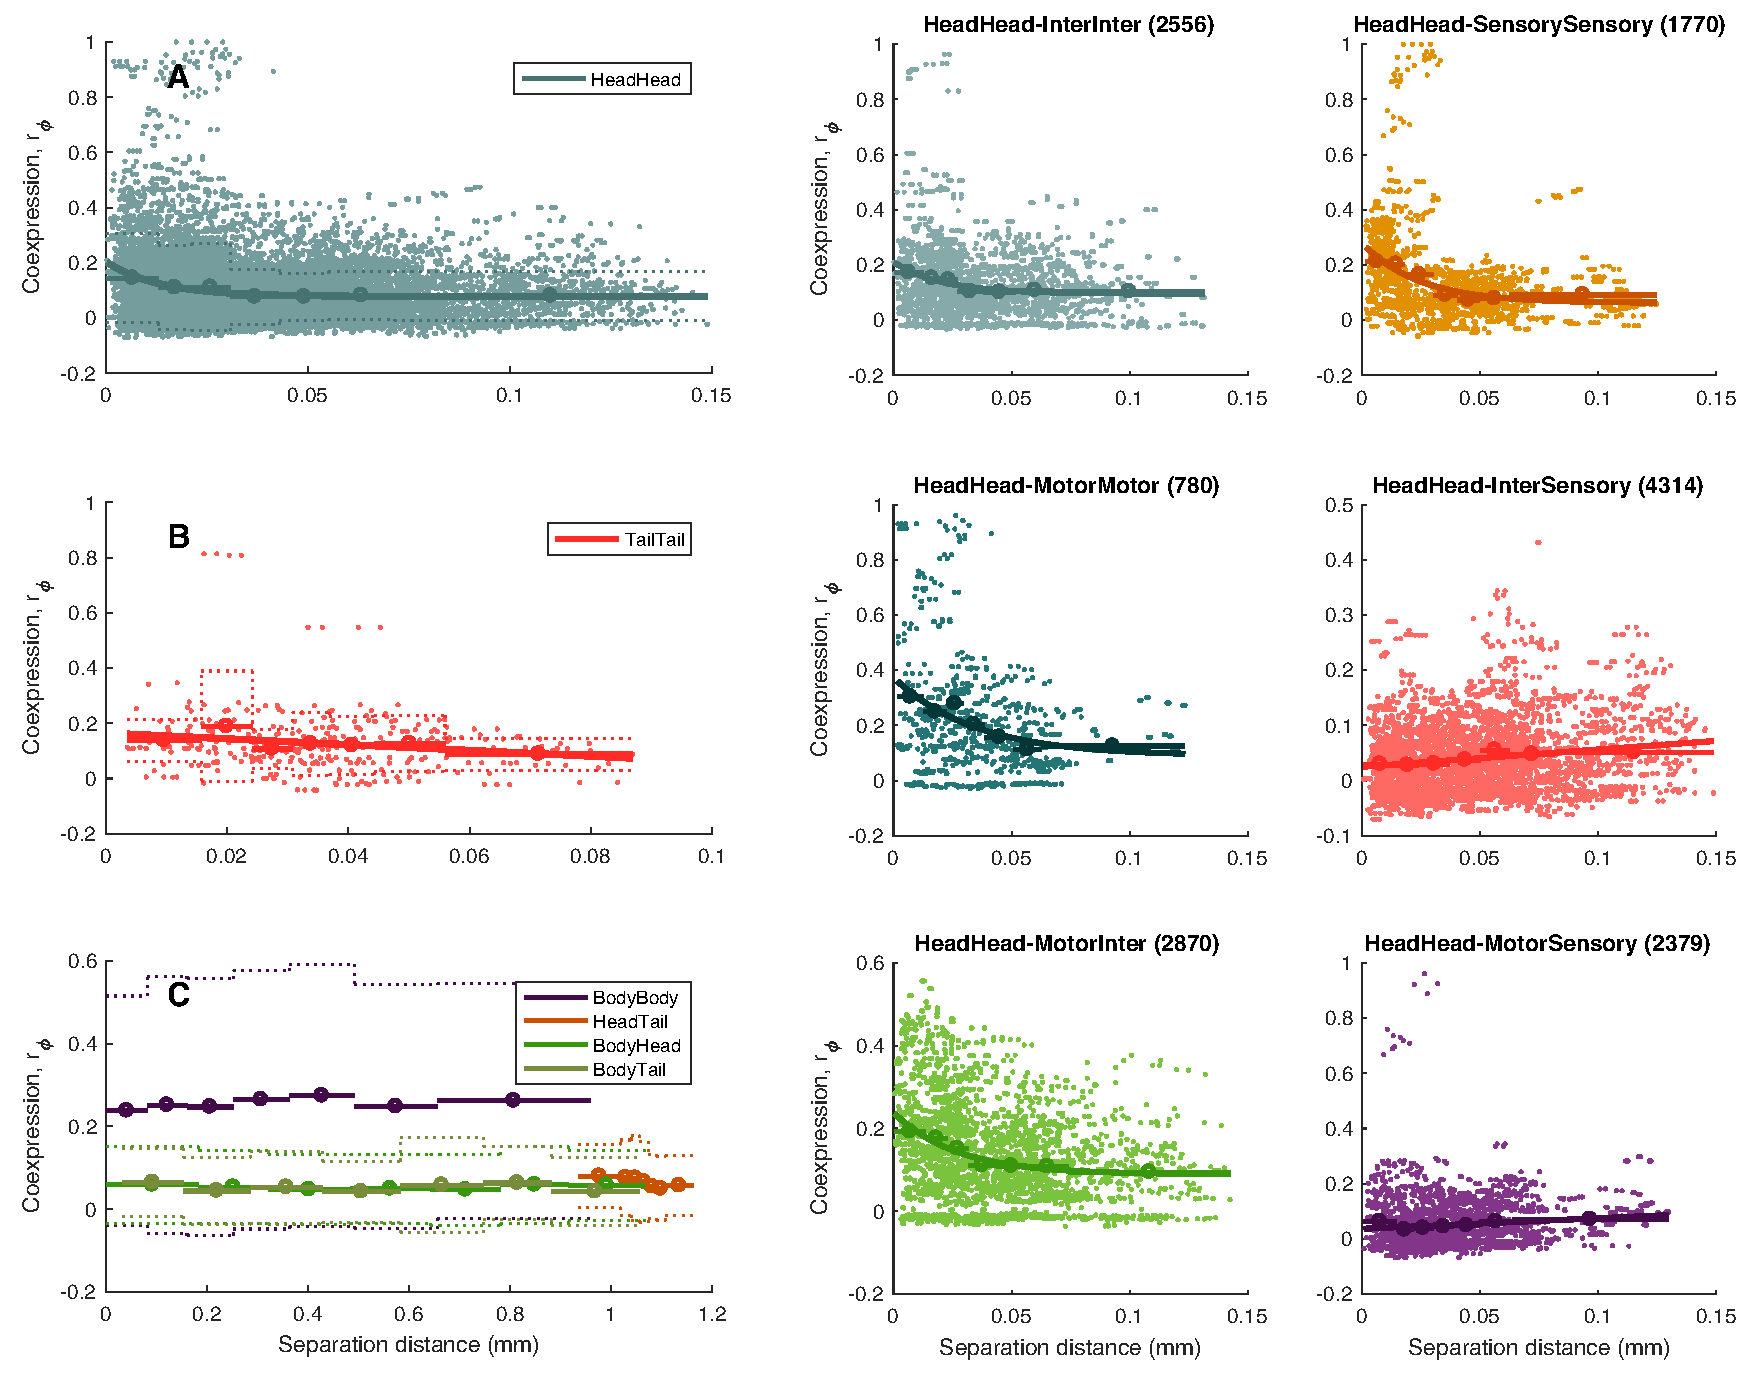
\includegraphics[width=1\textwidth]{DistanceCoexpression.pdf}
%     % 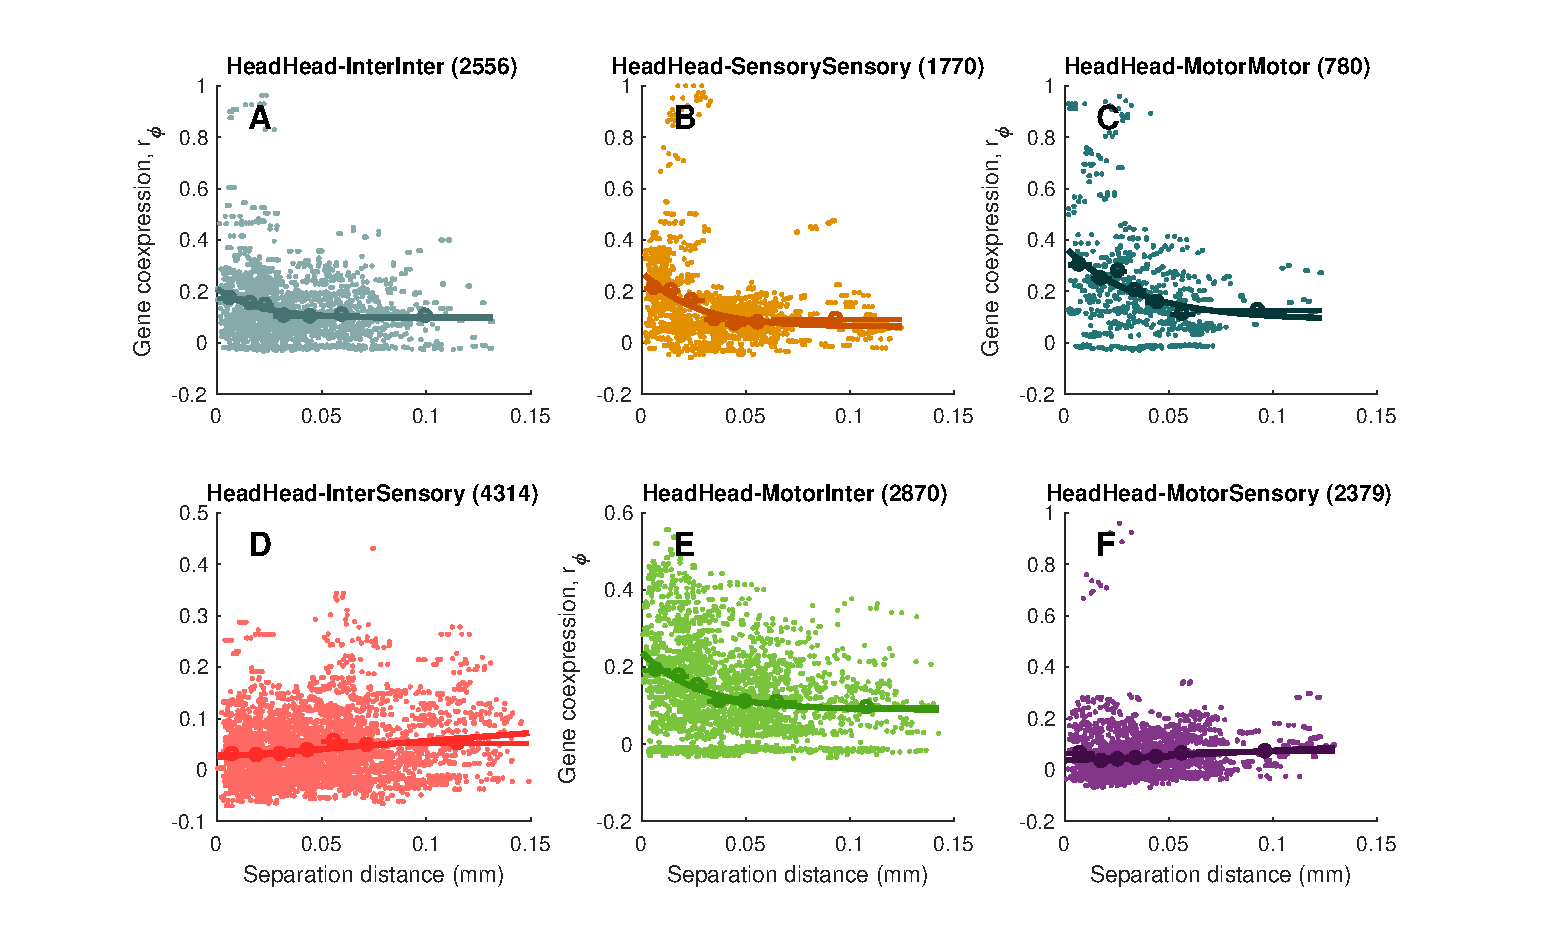
\includegraphics[width=1\textwidth]{coExpressionDistanceDetail.eps}
% \caption{
% \label{fig:S_distCoexp}
% \textbf{Gene coexpression decreases with separation distance within the head and tail.}
% Gene coexpression, $r_\phi$ (in all cases excluding left-right homologous pairs of neurons), is shown as a function of the pairwise separation distance between pairs of neurons (shown as the mean (solid) $\pm$ standard deviation (dotted) in seven equiprobable distance bins, with extent shown as horizontal bars), for \textbf{A} all pairs of neurons in the head, \textbf{B} all pairs of neurons in the tail, and \textbf{C} all other pairs (labeled).
% Scatters for all neuron pairs are added in \textbf{A} and \textbf{B}.
% An exponential relationship, $f(x) = a\exp(-bx) + c$, is fitted in \textbf{A} and \textbf{B}, revealing a slight decreasing trend in $r_\phi$ with distance, as per macroscopic mammalian brains \cite{Fulcher:2016ck, Krienen:2016eq}.
% Looking within the head, we find different spatial relationships as a function of neuron type, shown for \textbf{C} pairs of interneurons, \textbf{D} pairs of motor neurons, \textbf{E} motor-interneuron pairs, \textbf{F} pairs of sensory neurons, \textbf{G} interneuron-sensory neuron pairs, and \textbf{H} motor-sensory pairs.
% [[TODO: add labels for subplots C--H, label all axes? Change axis label to Gene coexpression, $r_\phi$ ]]
% }
% \end{figure}
% ------------------------------------------------------------------------------


% ------------------------------------------------------------------------------
% <<FeedInOutNodes.m>>
% ------------------------------------------------------------------------------
% % \paragraph*{S4 Fig.}
% % {\bf Neuron properties vary in therms of their connectivity relationship to hub nodes. }
% \begin{figure}[h]
% \centering
%     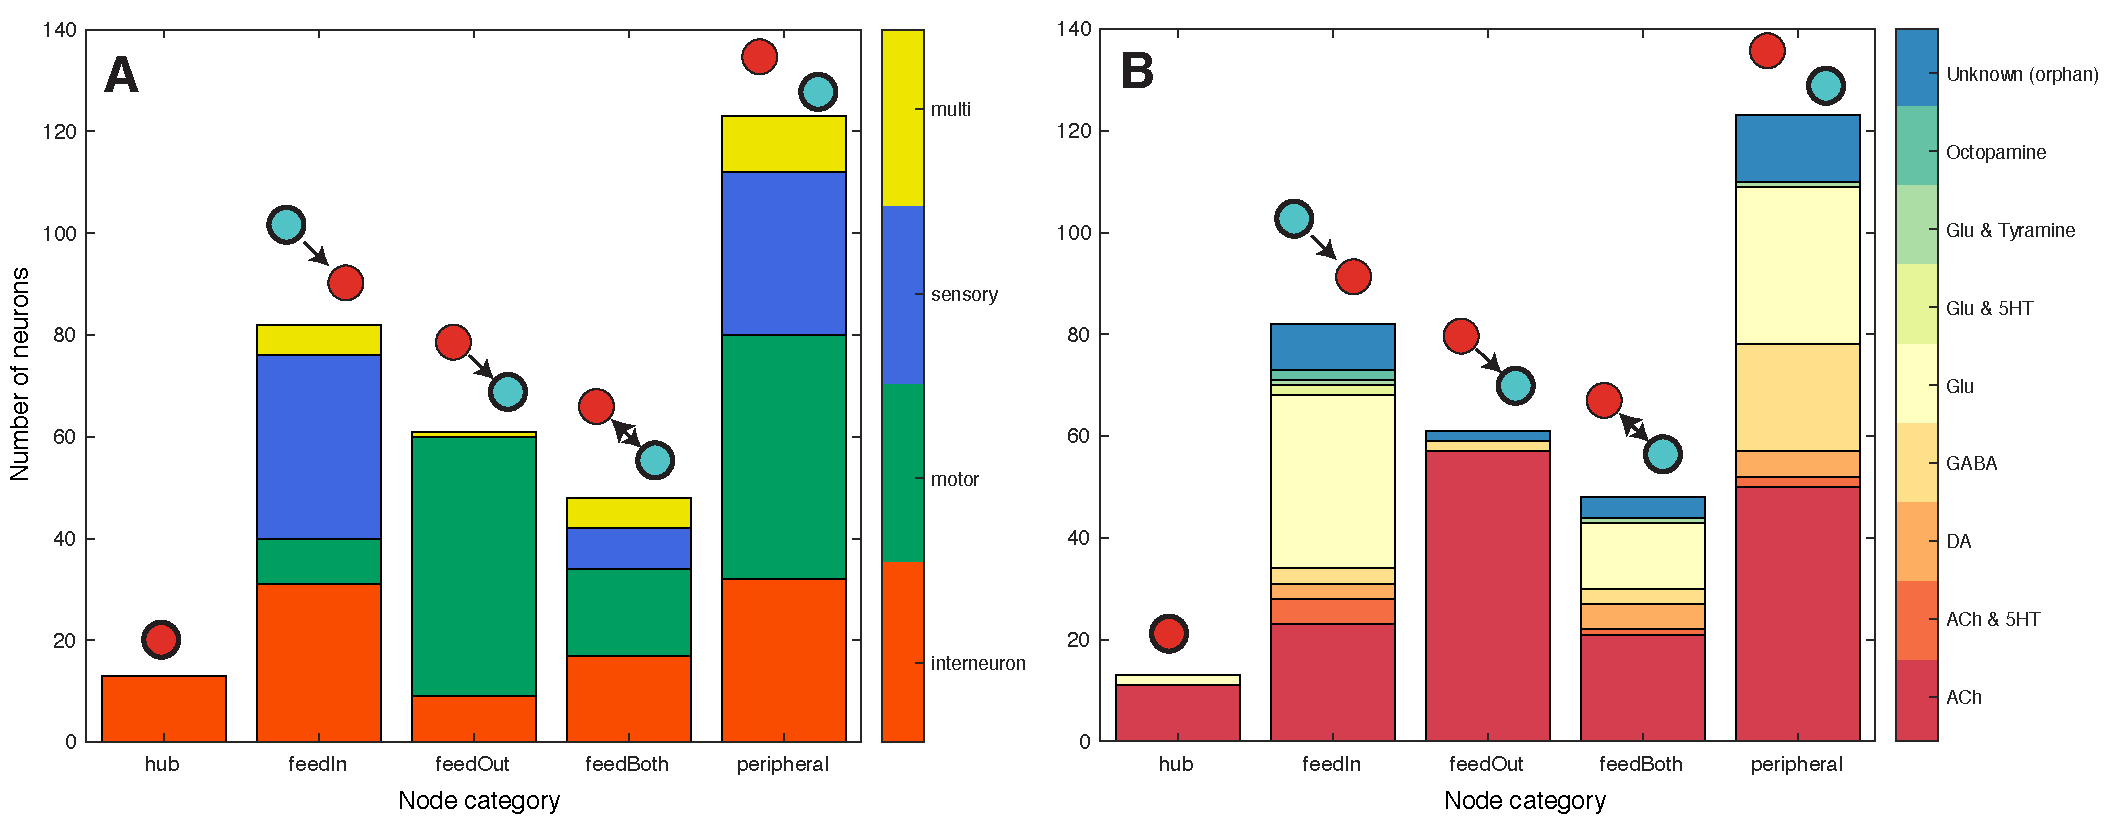
\includegraphics[width=1\textwidth]{FeedInOutNodesJustTwo.pdf}
% \caption{
% \textbf{Neuron properties vary in terms of their connectivity relationship to hub nodes.}
% Using a degree threshold for hubs, $k > 41$, we class all individual neurons into five mutually exclusive categories, shown schematically in the figures, for hubs (red) and nonhubs (light blue), as:
% (i) `hub' ($k>41$),
% and then classify nonhubs ($k\leq41$) as:
% (ii) `feedIn' (projects to a hub, but does not receive a projection from a hub),
% (iii) `feedOut' (receives a projection from a hub, but does project to a hub),
% (iv) `feedBoth' (receives a projection from, and projects to a hub),
% (v) `peripheral' (neither receives a projection from nor projects to a hub).
% We show the number of neurons in each of these fives classes that:
% \textbf{A} is an interneuron (orange), motor neuron (green), sensory neuron (blue), or multimodal (yellow),
% % \textbf{B} is in the head (gray), body (purple), or tail (red),
% \textbf{B} uses one of nine neurotransmitter systems (labeled).
% \label{fig:S_feedInOutNodes}
% [[TODO: Come up with new names for nodes that don't confuse with edge names. Labels not visible for B]]
% }
% \end{figure}
% ------------------------------------------------------------------------------
% <<networkRC.m>>
% \paragraph*{S7 Fig.}
\paragraph*{S4 Fig.}
\label{S4_Fig}
{\bf Weighted and unweighted rich-club analyses yield similar results.}
   (A) Degree distribution of the \emph{C. elegans} connectome.
    Neurons are labeled to four types as in the legend.
    (B)
    Normalized weighted rich-club coefficient, $\Phi_\mathrm{norm}^\mathrm{weighted}$ (i.e., topology fixed and weights randomized in the null model, shown orange), and
    normalized mixed rich-club coefficient, $\Phi_\mathrm{norm}^\mathrm{mixed}$ (i.e., both topology and weights mixed in the null model, shown green) are plotted as a function of the degree, $k$, at which hubs are defined (as neurons with degree $>k$) \cite{Alstott2014}.
    Circles indicate values of $\Phi_\mathrm{norm}$ that are significantly higher than an ensemble of 1\,000 degree-matched null networks (Welch's $t$-test, $p < 0.05$).
    Compared to topological rich-club analysis presented in the main text, here the weights of the connections are also accounted for when calculating the rich club coefficient.
    In the case of the weighted rich-club coefficient, the topology for the null models was kept stable and only the weights of the connections randomized. Results presented here show that connections between higher degree nodes are stronger than expected by chance.
    On the other hand, in the mixed rich club coefficient both the topology and weights are randomized, therefore we see the combined effect of both types.
    Distinction between the different null models is discussed in detail in \cite{Alstott2014}.
    These results show that connections between high degree nodes are both denser and stronger than expected by chance.


% ------------------------------------------------------------------------------
% <<RichClub.m>>
% \paragraph*{S8 Fig.}
 %{\bf Weighted rich club organisation of the connectome.}
%\begin{figure}[!h]
%\centering
 %   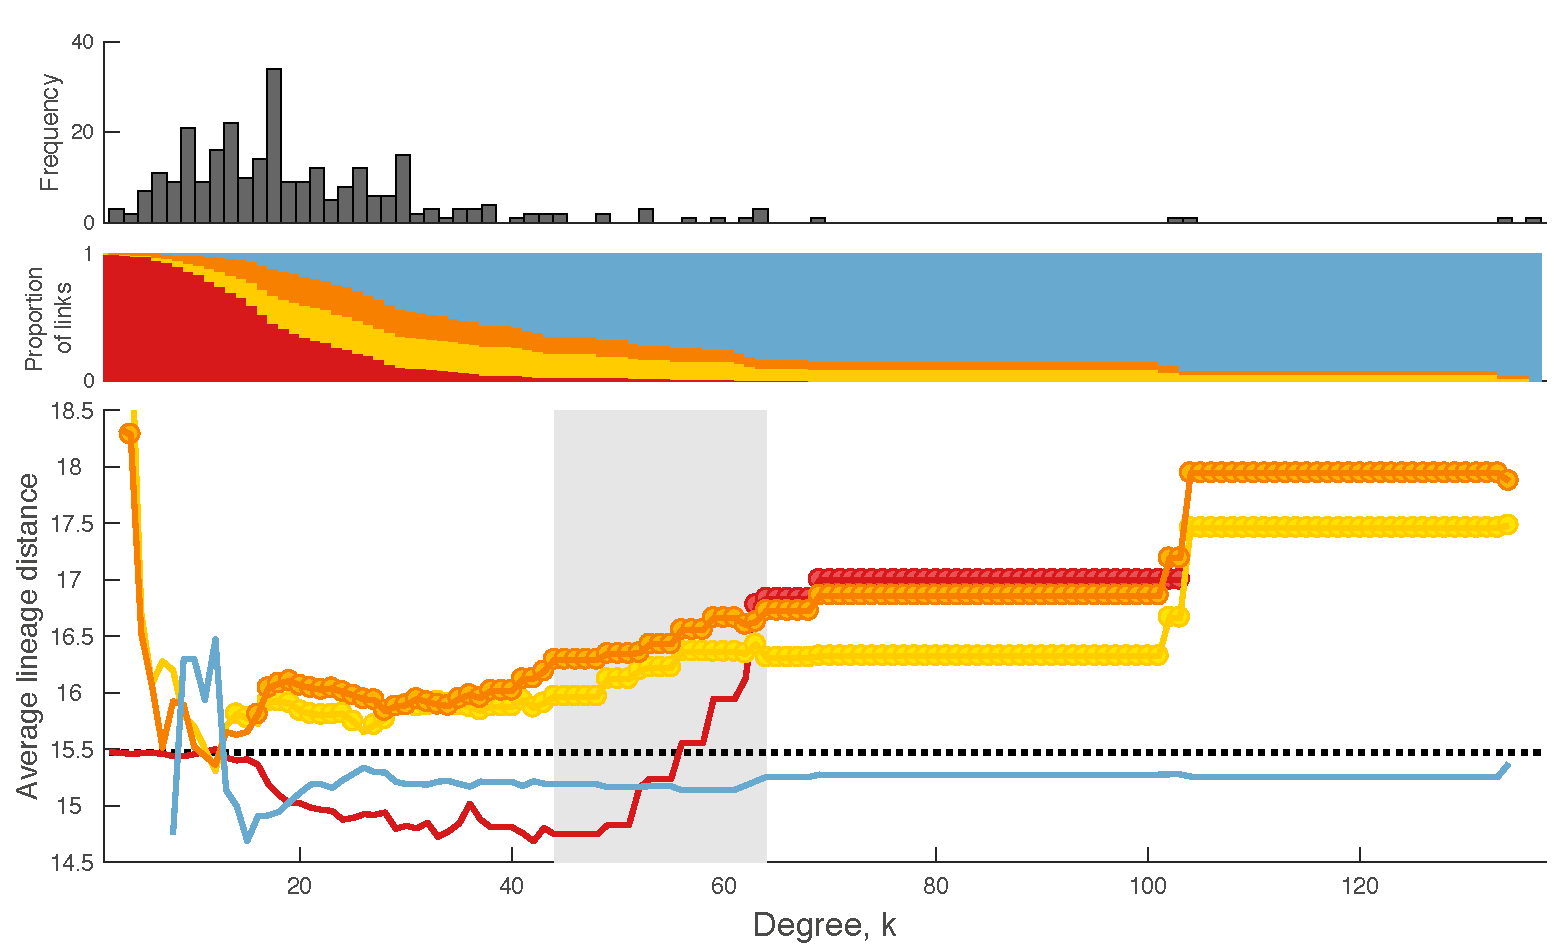
\includegraphics[width=1\textwidth]{lineageDistanceRPF.pdf}
 %   \caption{
 %   \textbf{Lineage distance between pairs of neurons for different connection types as a function of the degree at which hubs are defined, $k$.}
%    \emph{Top}: Degree distribution.
%\emph{Middle}: proportion of connections that are `rich' (hub$\rightarrow$hub, red), `feed-in' (nonhub$\rightarrow$hub, yellow), `feed-out' (hub$\rightarrow$nonhub, orange), and `peripheral' (nonhub$\rightarrow$nonhub, blue) as a function of the degree threshold, $k$, used to define hubs.
%Note that at high $k$, most neurons are labeled as nonhubs, and hence the vast majority of connections are `peripheral'.
%\emph{Lower}: Mean lineage distance for each connection type as a function of $k$.
%Lineage distance across all network links shown as a dotted black line; the topological rich-club regime %(determined from the network topology, cf. Fig.~\ref{fig:Fig5}) is shaded gray.
%Circles indicate a statistically significant increase or decrease in birth time difference in a given link %type relative to the rest of the network (two-sided Welch’s t test; $p < 0.05$).
%}
%\label{fig:Lineagek}
%\end{figure}
% <<RichClub.m>>

% ------------------------------------------------------------------------------
% \paragraph*{S9 Fig.}
% {\bf Mean birth time difference as a function of degree for different link types}
%\begin{figure}[!h]
%\label{BirthTimesk}
%\centering
 %   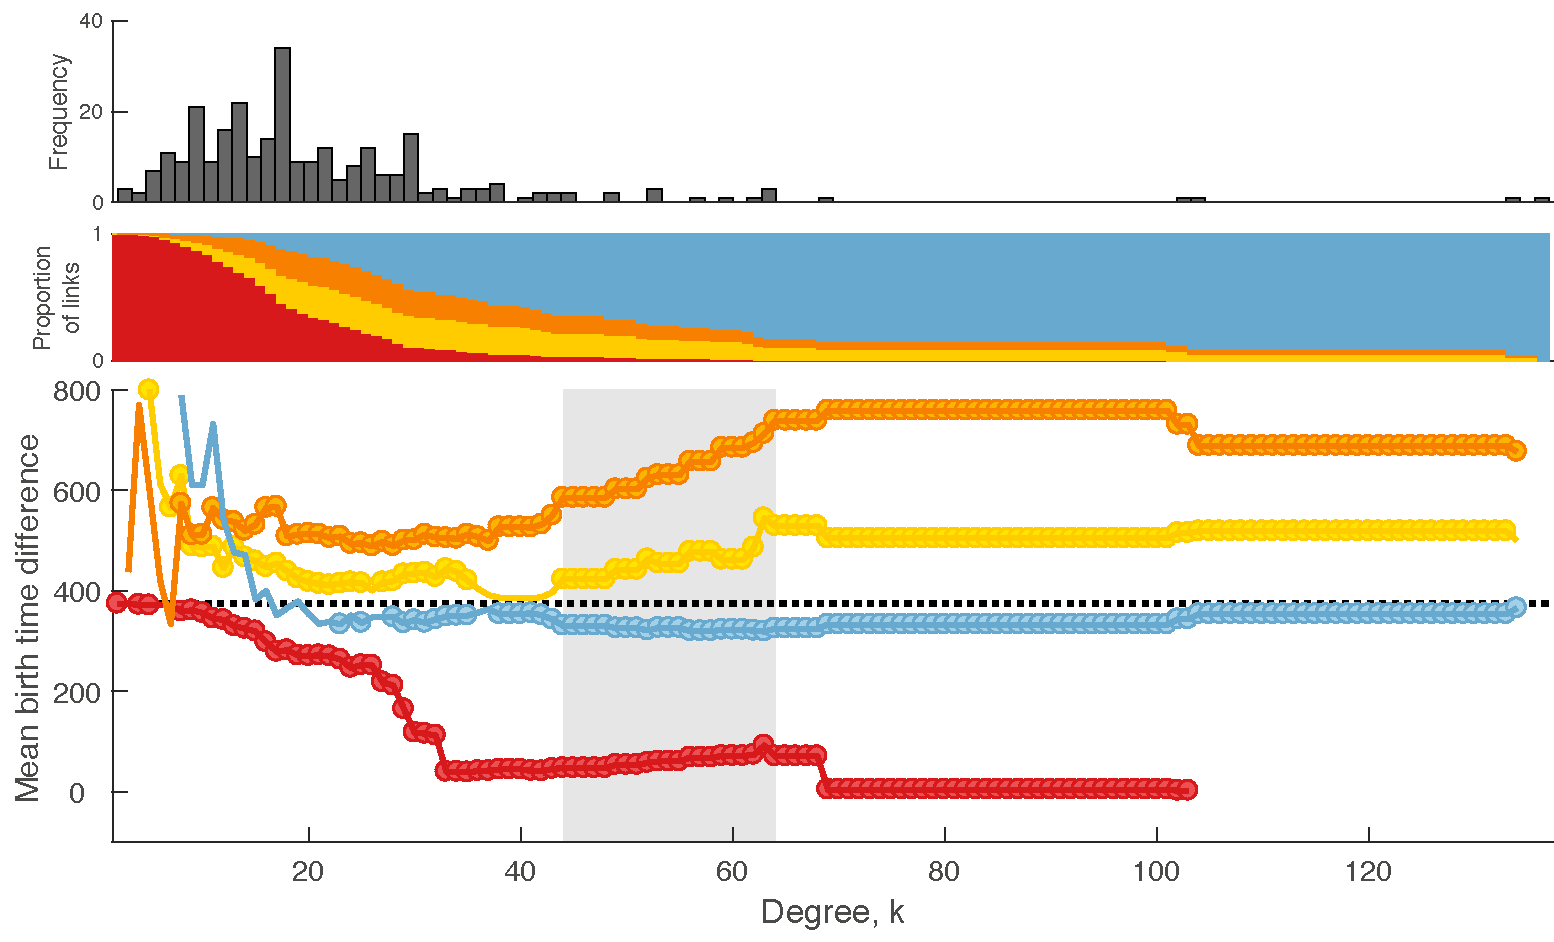
\includegraphics[width=1\textwidth]{birthTimeRPFALL.pdf}
 %   \caption{
 %   \textbf{Birth time difference between pairs of neurons for different connection types as a function of the degree at which hubs are defined, $k$.}
%\emph{Top}: Degree distribution.
%\emph{Middle}: proportion of connections that are `rich' (hub$\rightarrow$hub, red), `feed-in' (nonhub$\rightarrow$hub, yellow), `feed-out' (hub$\rightarrow$nonhub, orange), and `peripheral' (nonhub$\rightarrow$nonhub, blue) as a function of the degree threshold, $k$, used to define hubs.
%Note that at high $k$, most neurons are labeled as nonhubs, and hence the vast majority of connections are `peripheral'.
%\emph{Bottom}: Mean birth time difference for each connection type as a function of $k$.
%The mean birth time difference across all network links shown as a dotted black line; the topological rich-club regime (determined from the network topology, cf. Fig.~\ref{fig:Fig5}) is shaded gray.
%Circles indicate a statistically significant increase or decrease in birth time difference in a given link type relative to the rest of the network (two-sided Welch's $t$ test; $p < 0.05$).
%}
%\end{figure}

% propTypesDegree(C) script
%\paragraph*{S6 Fig.}
%{\bf Neuron type and neurotransmitter as a function of degree}
%\begin{figure}[!h]
%\label{S7_Fig}
%\centering
%    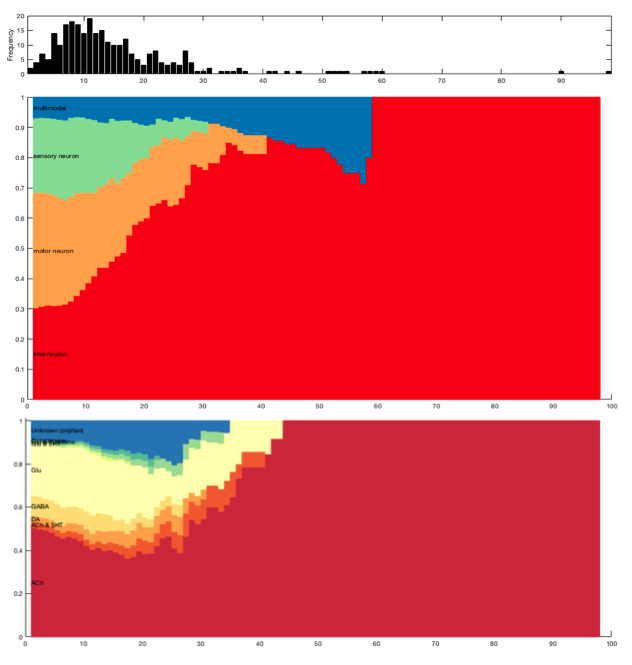
\includegraphics[width=0.7\textwidth]{TypeTransmitterDegree}
%\end{figure}

% ------------------------------------------------------------------------------
% hubConnectionDistance(C)
% ------------------------------------------------------------------------------
\paragraph*{S5 Fig.}
\label{S5_Fig}
{\bf Rich and non-rich connections in the \emph{C. elegans} connectome, categorized by the  anatomical location of the source and target neurons.}
   Hub-hub connections (`rich') are shown red, and all other connections (`non-rich', i.e., feeder and peripheral) are shown gray, where hubs are defined as neurons with degree, $k > 44$.
Anatomical locations are labeled as `head', `body', and `tail', and each connection is labeled according to its source and target neurons, labeled on the vertical axis in the form `Source-Target'.
% corresponding to the lowest threshold at which the \emph{C. elegans} connectome exhibits rich-club organization.
The plot shows that the increased separation distance between connected hubs relative to other types of connected neurons is driven by a relative increase in long-range connections between the head and tail.

% ------------------------------------------------------------------------------
% <<plot_disstributionsSUPP.m>>
% ------------------------------------------------------------------------------

% \paragraph*{S6 Fig.}
% {\bf Coexpression for rich, feeder and peripheral links as a function of degree.}
%\begin{figure}[h]
%\centering
%    \includegraphics[width=1\textwidth]{distributionsSUPP2.pdf}
%    \caption{
%\textbf{Distributions of correlated gene expression for different types of connectome edges.}
%Violin plots of the distribution of CGE, $r_\phi$, between reciprocally connected (219 pairs), unidirectionally connected (1\,721) and unconnected (36\,749 pairs) pairs of neurons; also for pairs of neurons labeled as peripheral, feed-in, feed-out, and rich, where hubs are neurons with degree $k>44$. The median of each distribution shown as a horizontal line.
% Connections between symmetrical (left/right) pairs of neurons are excluded from the analysis.
%CGE is increased in connected (electrical or chemical; reciprocally or unidirectionally) pairs of neurons relative to unconnected pairs ($p = 1.8 \times 10^{-78}$, Wilcoxon rank sum test).
%CGE between neurons connected via gap junctions is significantly higher than between neurons connected via chemical synapses ($p = 5.4 1\times 0^{-22}$, Wilcoxon rank sum test). CGE is significantly higher between hubs (rich links) compared to feeder ($p = 5 \times 10^{-22}$, Wilcoxon rank sum test) and peripheral ($p = 3.9 \times 10^{-19}$, Wilcoxon rank sum test) links. Feed-out links show significantly higher CGE than both feed-in ($p = 1.9 \times 10^{-6}$, Wilcoxon rank sum test) and peripheral links ($p = 4.5 \times 10^{-12}$, Wilcoxon rank sum test).
%\label{fig:S_RFPdistributions}
%}
%\end{figure}

\end{document}
